%!TEX root = index.tex
\chapter[Resultados]{Resultados}
\label{chap:resultados}

Os resultados deste trabalho são a análise de desempenho dos algoritmos propostos, em termos de precisão, abrangência e tempo computacional, mediante a mudanças em suas variáveis de importância (Tabela \ref{tab:variaveis}).

Além disso, as metodologias de solução de cada um dos sistemas serão debatidas, de modo a explorar casos de uso particulares e a propor melhorias nos métodos computacionais. Serão respondidas perguntas como ``O que acontece com itens ou usuários sem nenhuma avaliação?'' e ``Qual o desempenho dos métodos para outros bancos de dados?''.

\begin{table}[hp]
\begin{center}
    \caption{Parâmetros de influência no desempenho dos algoritmos de recomendação}
    \label{tab:variaveis}
    \begin{tabular}{  | p{2cm} | p{7cm} | p{3.5cm} | } 
    \hline
    \textbf{Variável} & \textbf{Descrição} & \textbf{Valor padrão}  \\ \hline
    $N$ & Tamanho da lista de recomendação & $20$ \\ \hline   
    $T$ & Percentual da base de aprendizado na validação cruzada & $75\%$ \\ \hline
    $H$ & Percentual de avaliações ``escondidas'' dos usuários-teste na validação cruzada & $75\%$ \\ \hline
    $M$ & Valor mínimo para avaliações positivas & $2$ \\ \hline
    $k$ & Número de vizinhos mais próximos & $10$ \\ \hline
    $\mathcal{F}$ & Conjunto de atributos dos itens & Todos atributos \\ \hline
    $d^f$ & Medida de distância entre atributos & $\left|\left|\cdot\right|\right|^f$ \\ \hline
    $w_f$ & Pesos dos atributos & $w_f>0$ \\ \hline
    \end{tabular}
\end{center}
\end{table}
%- diferenca entre NA e 0

\section{Tamanho da lista de recomendações $N$} % (fold)
\label{sec:tamanho_da_lista_de_recomenda_es_}

Assim como mostra a literatura, a medida que o tamanho da lista de recomendações aumenta, a precisão cai e a abrangência cresce (Figuras \ref{fig:precision_N} e \ref{fig:recall_N}). A primeira decresce com $N$ porque a quantidade de itens sugeridos se torna excessivamente maior que a quantidade de itens positivamente avaliados pelos usuários-teste. A segunda, por sua vez, cresce com $N$ porque a probabilidade de sugerirmos itens relevantes para o usuário aumenta quando sugerimos mais itens. Para $N=\left|\mathcal{I}\right|$, a abrangência atinge $100\%$, pois todos os itens teriam sido recomendados.

O método UP supera os dois outros algoritmos para todos os valores de $N$, tanto em precisão quanto em abrangência, como se observa pelo gráfico das medidas $F_1$.

\begin{figure}[htp]
    \begin{center}
    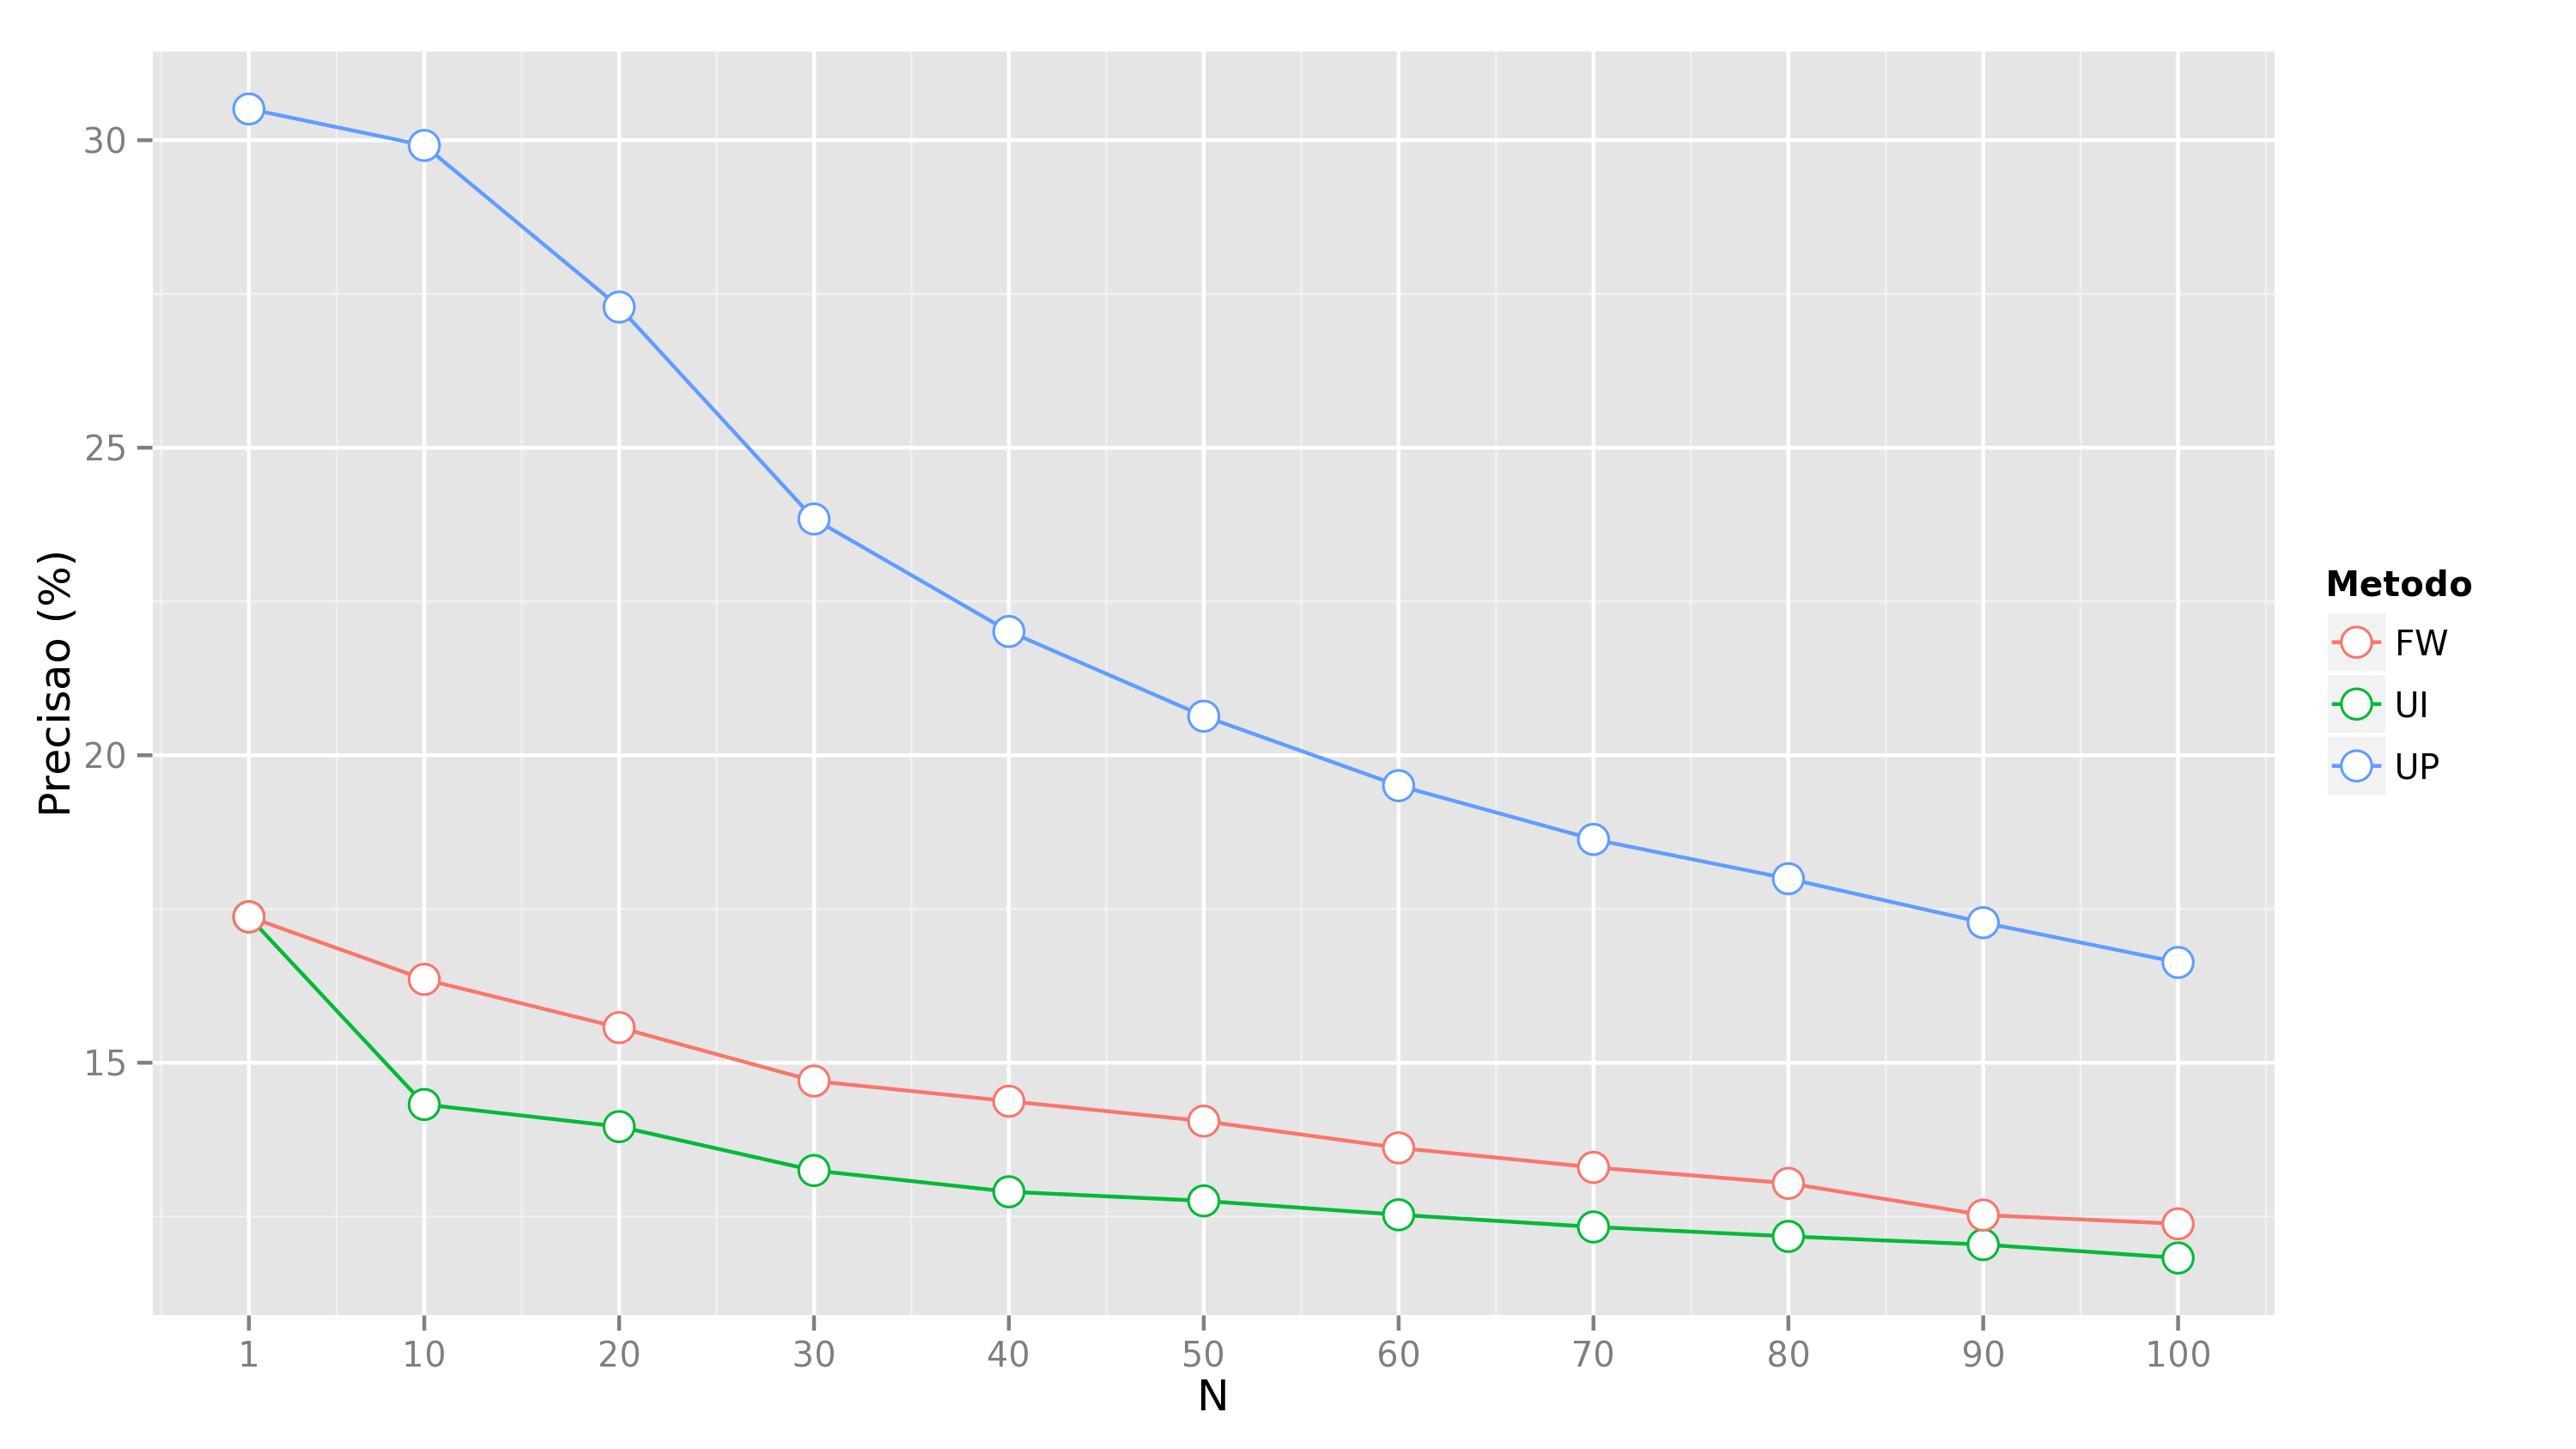
\includegraphics[width=1\textwidth]{img/precision_N}
    \end{center}
    \caption{Precisão em função do tamanho da lista de recomendações $N$}
    \label{fig:precision_N}
\end{figure}


\begin{figure}[htp]
    \begin{center}
    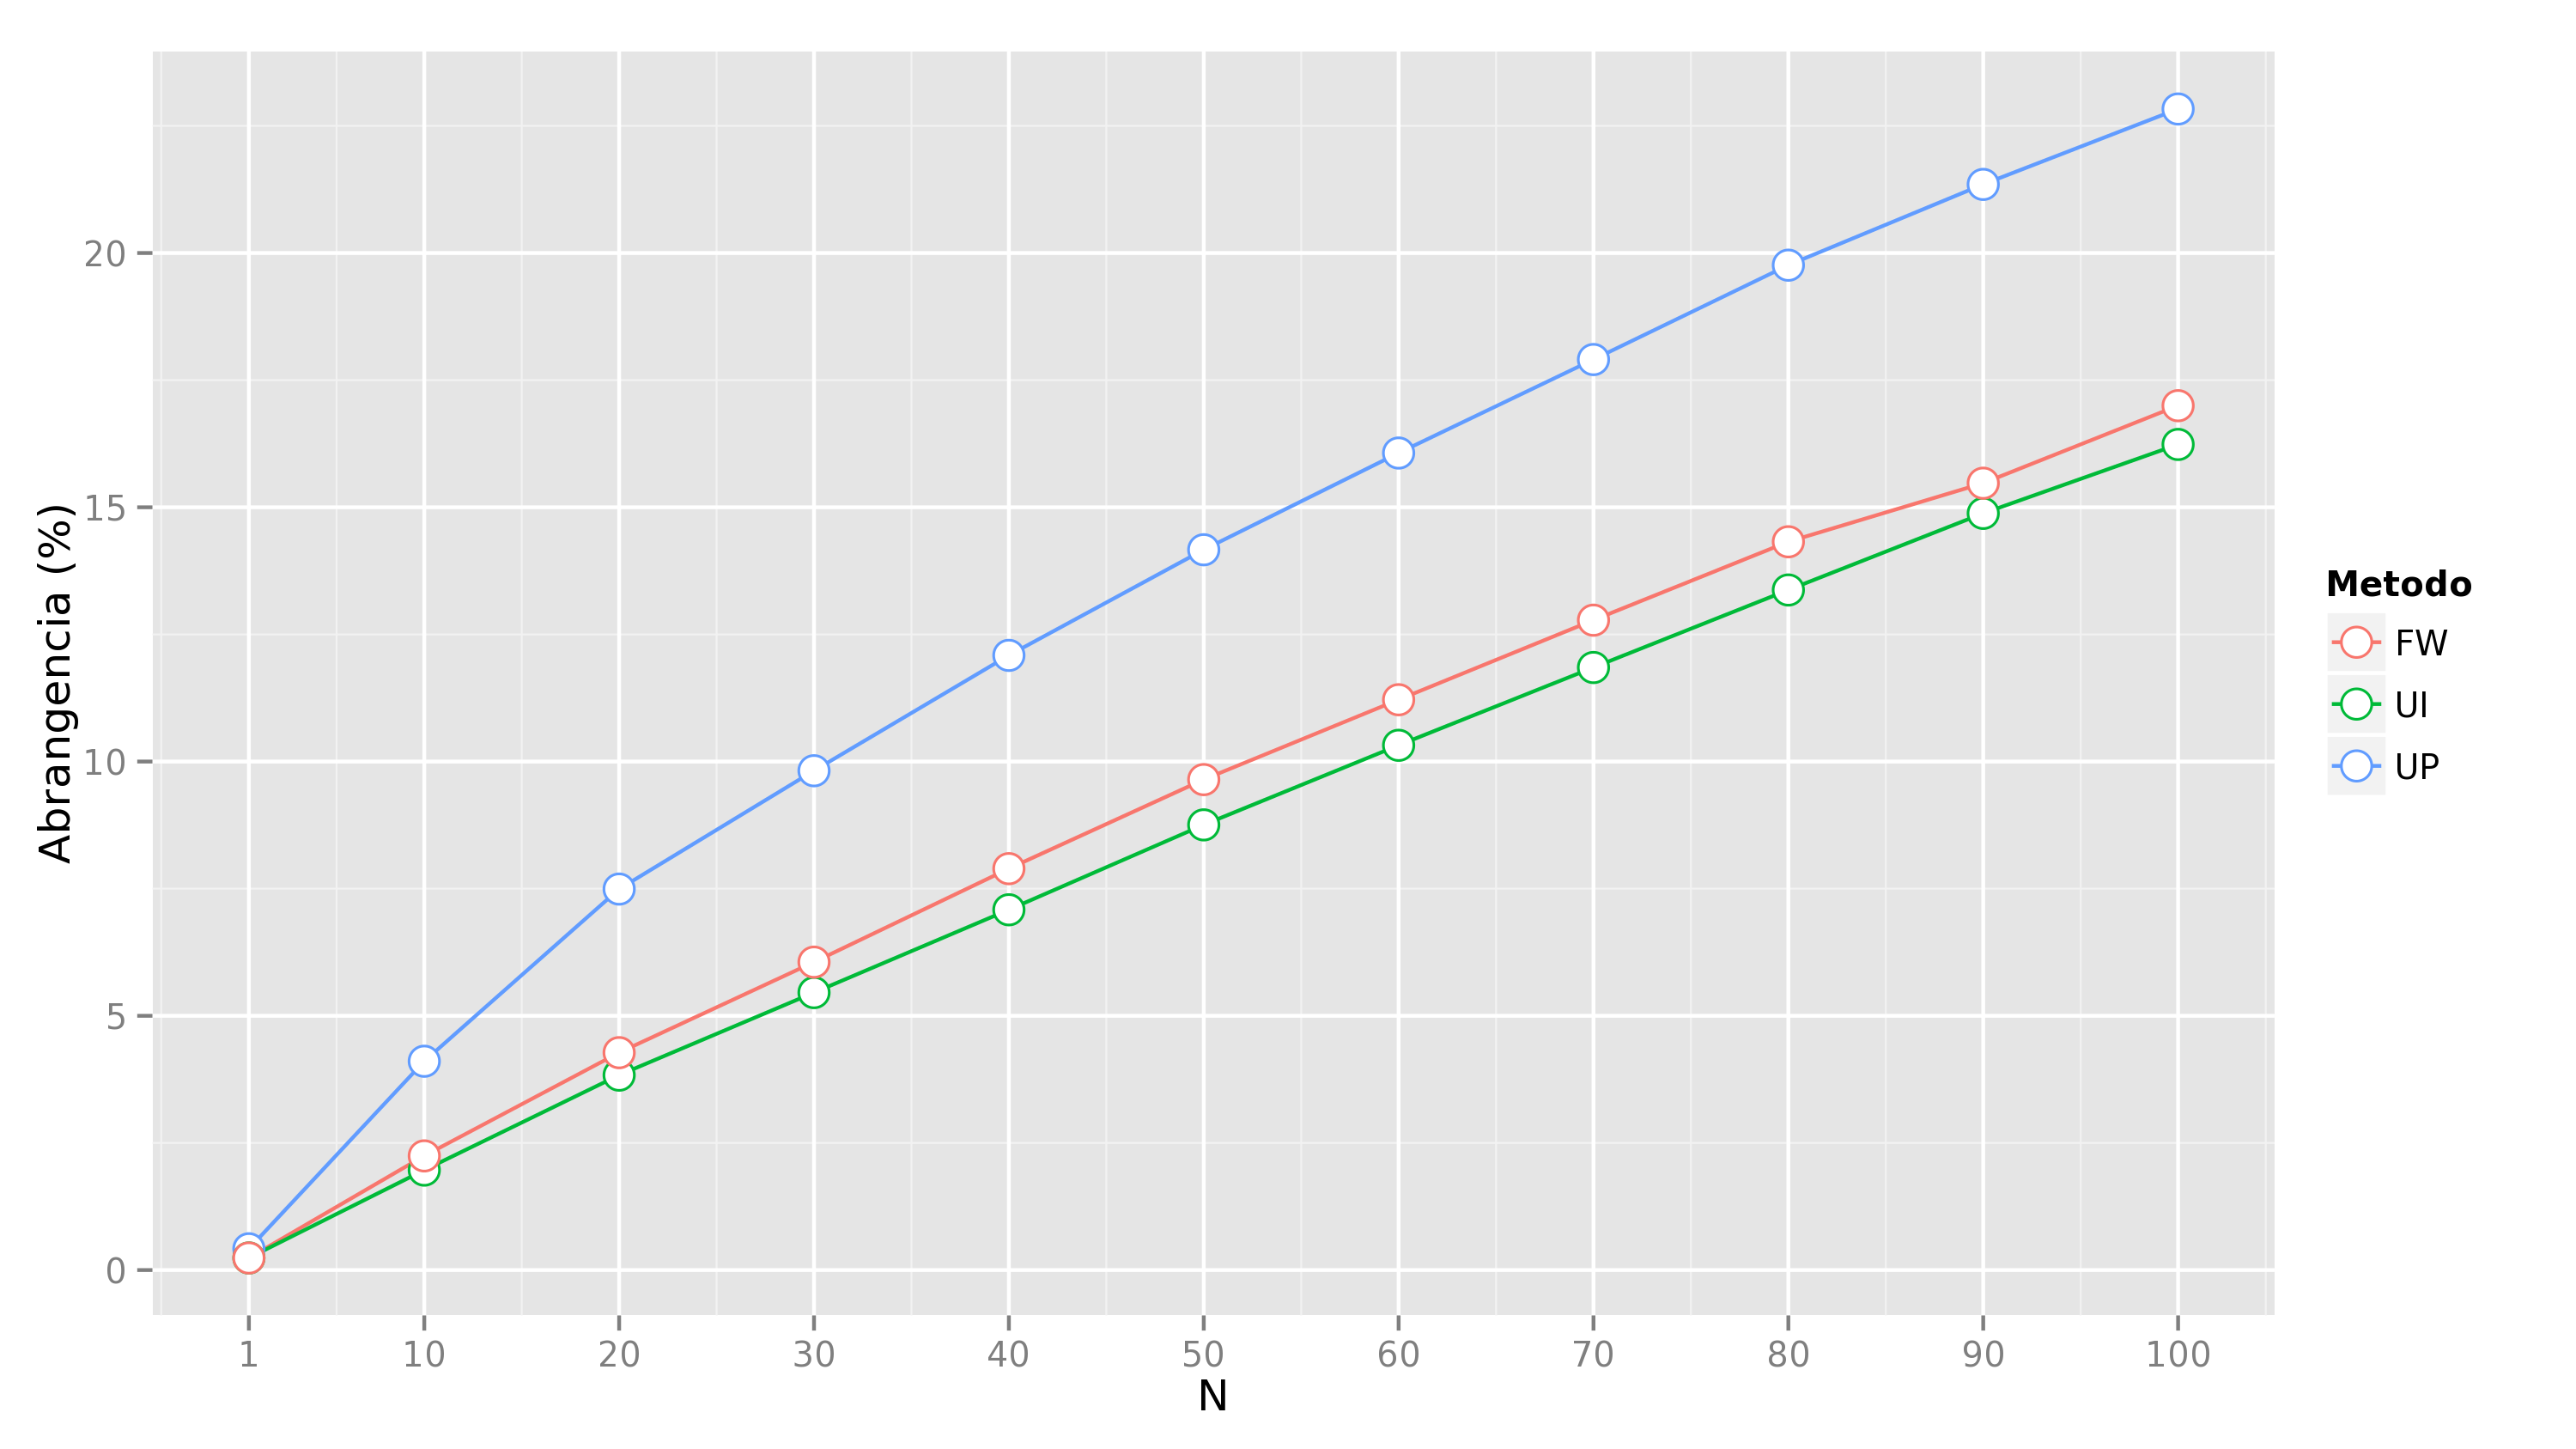
\includegraphics[width=1\textwidth]{img/recall_N}
    \end{center}
    \caption{Abrangência em função do tamanho da lista de recomendações $N$}
    \label{fig:recall_N}
\end{figure}

\begin{figure}[htp]
    \begin{center}
    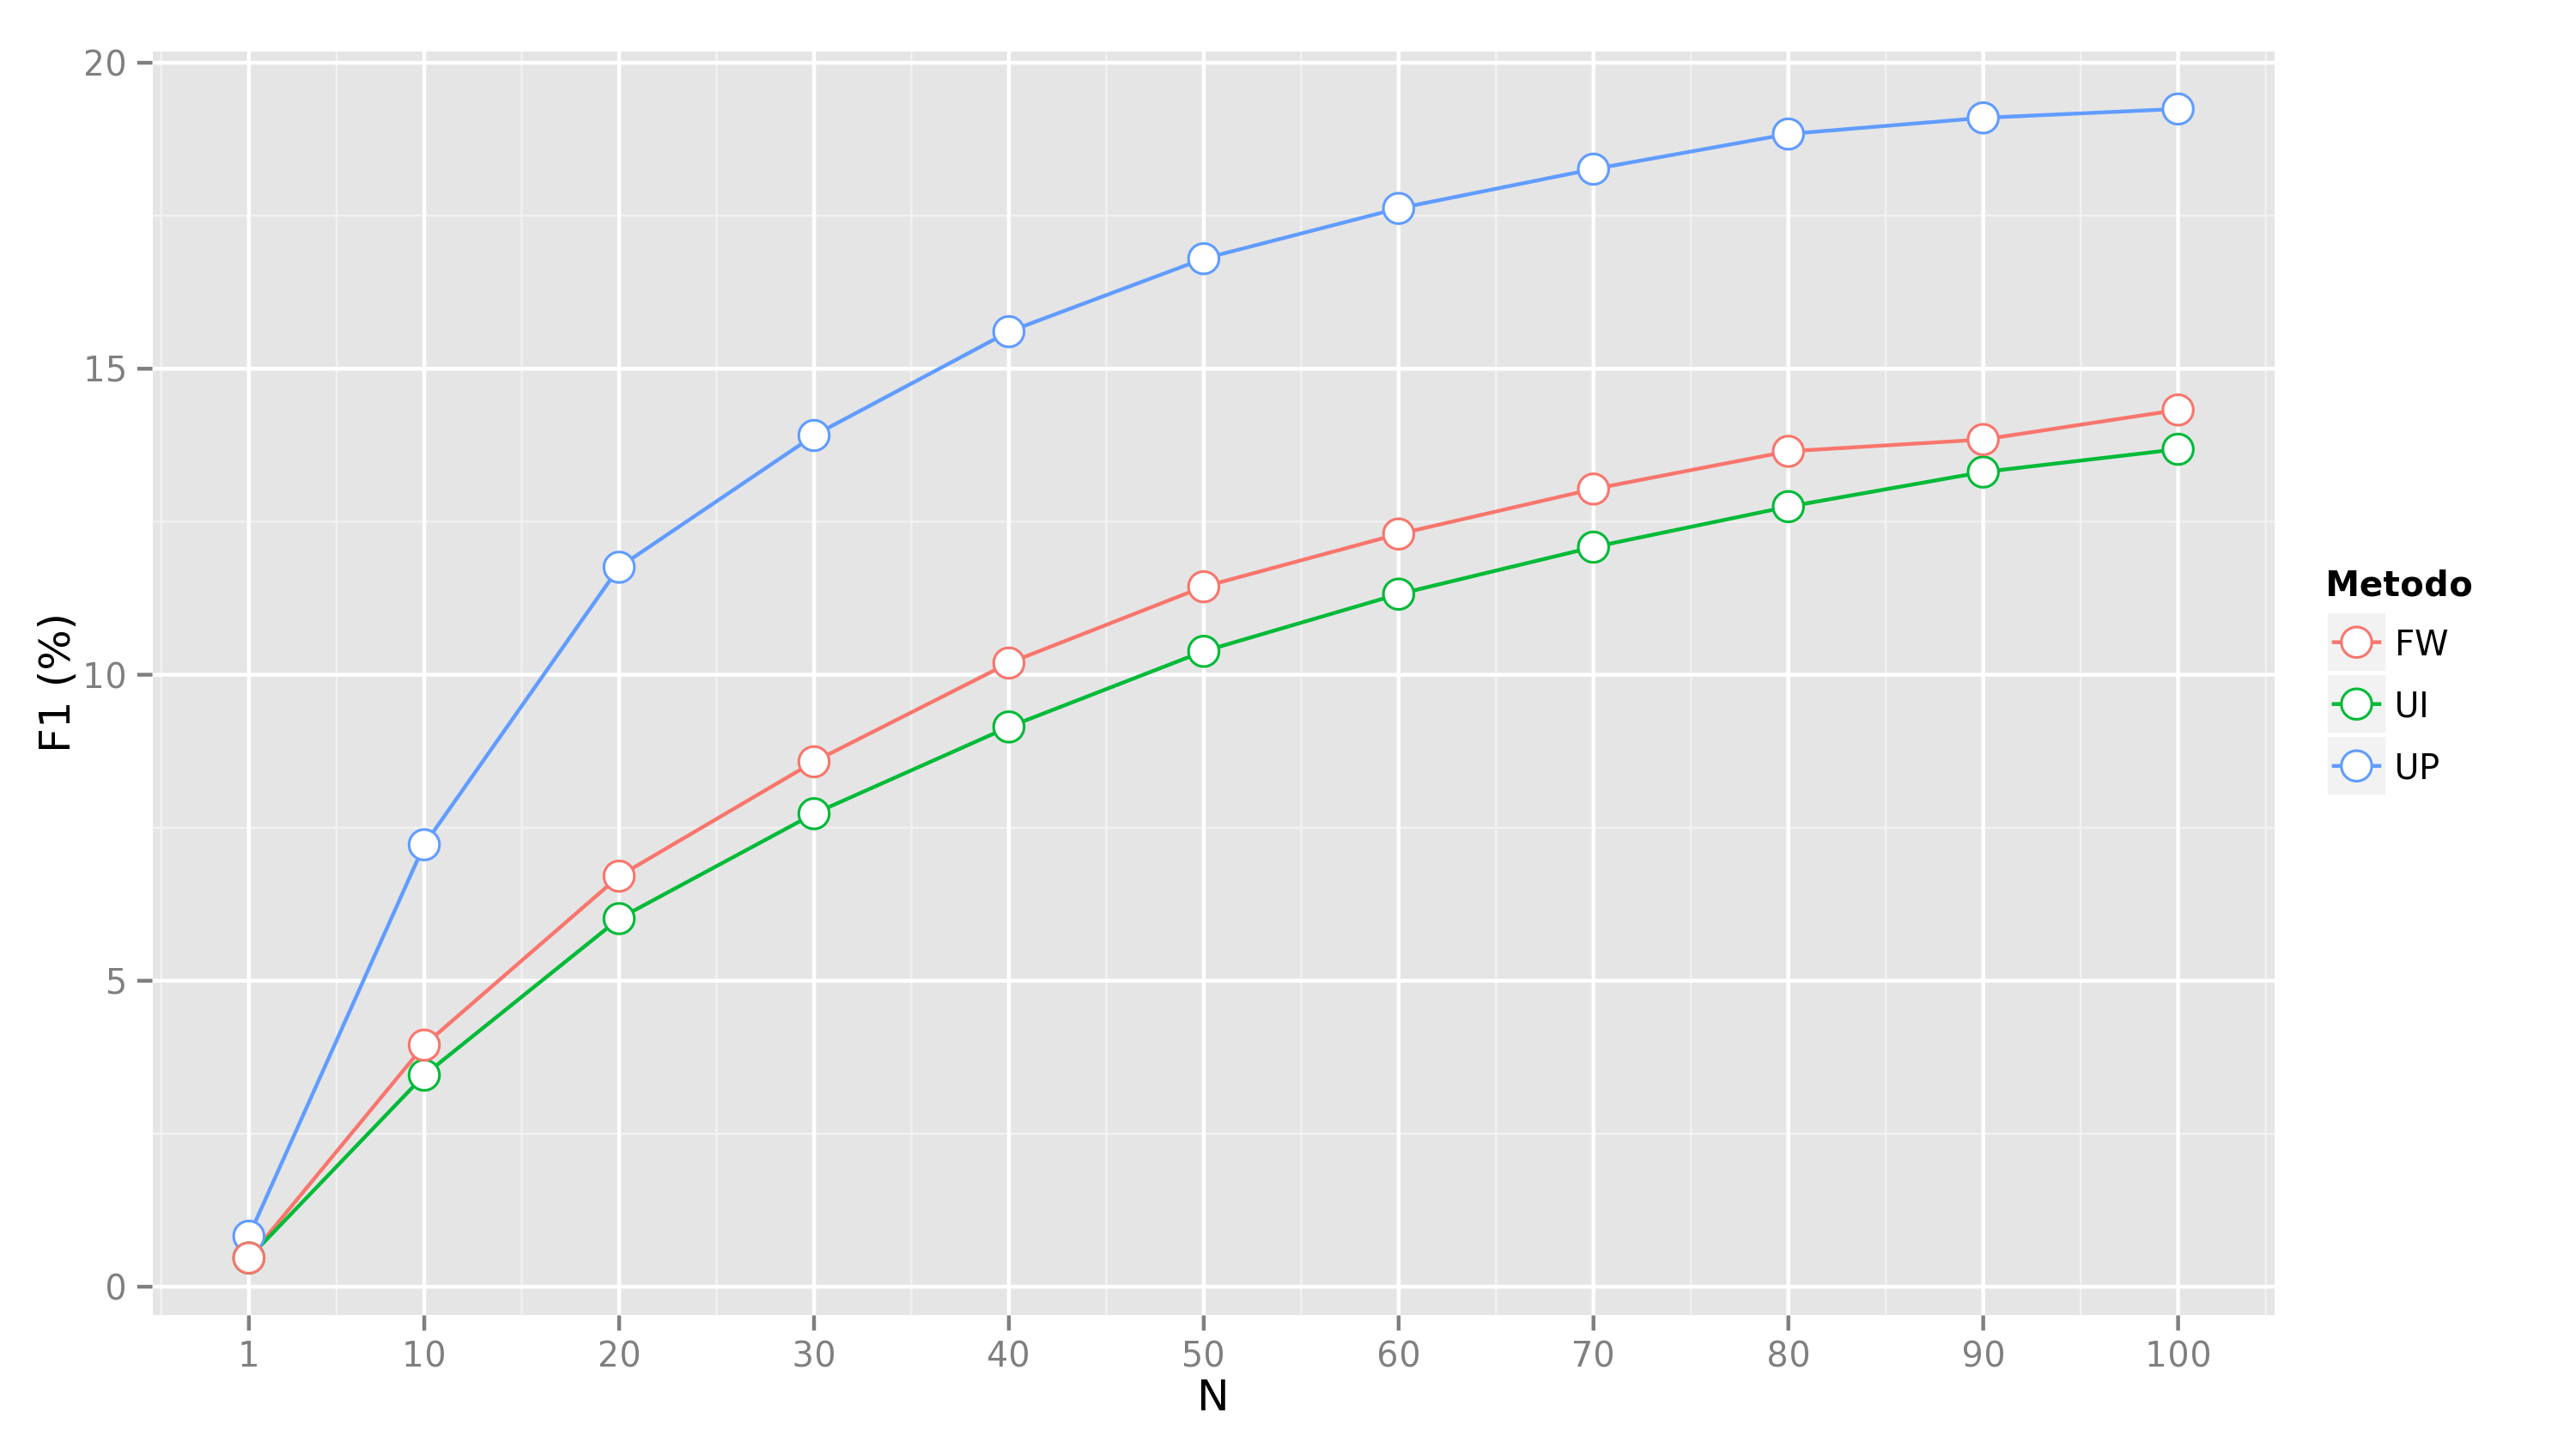
\includegraphics[width=1\textwidth]{img/F1_N}
    \end{center}
    \caption{Medida $F_1$ em função do tamanho da lista de recomendações $N$}
    \label{fig:F1_N}
\end{figure}

\begin{figure}[htp]
    \begin{center}
    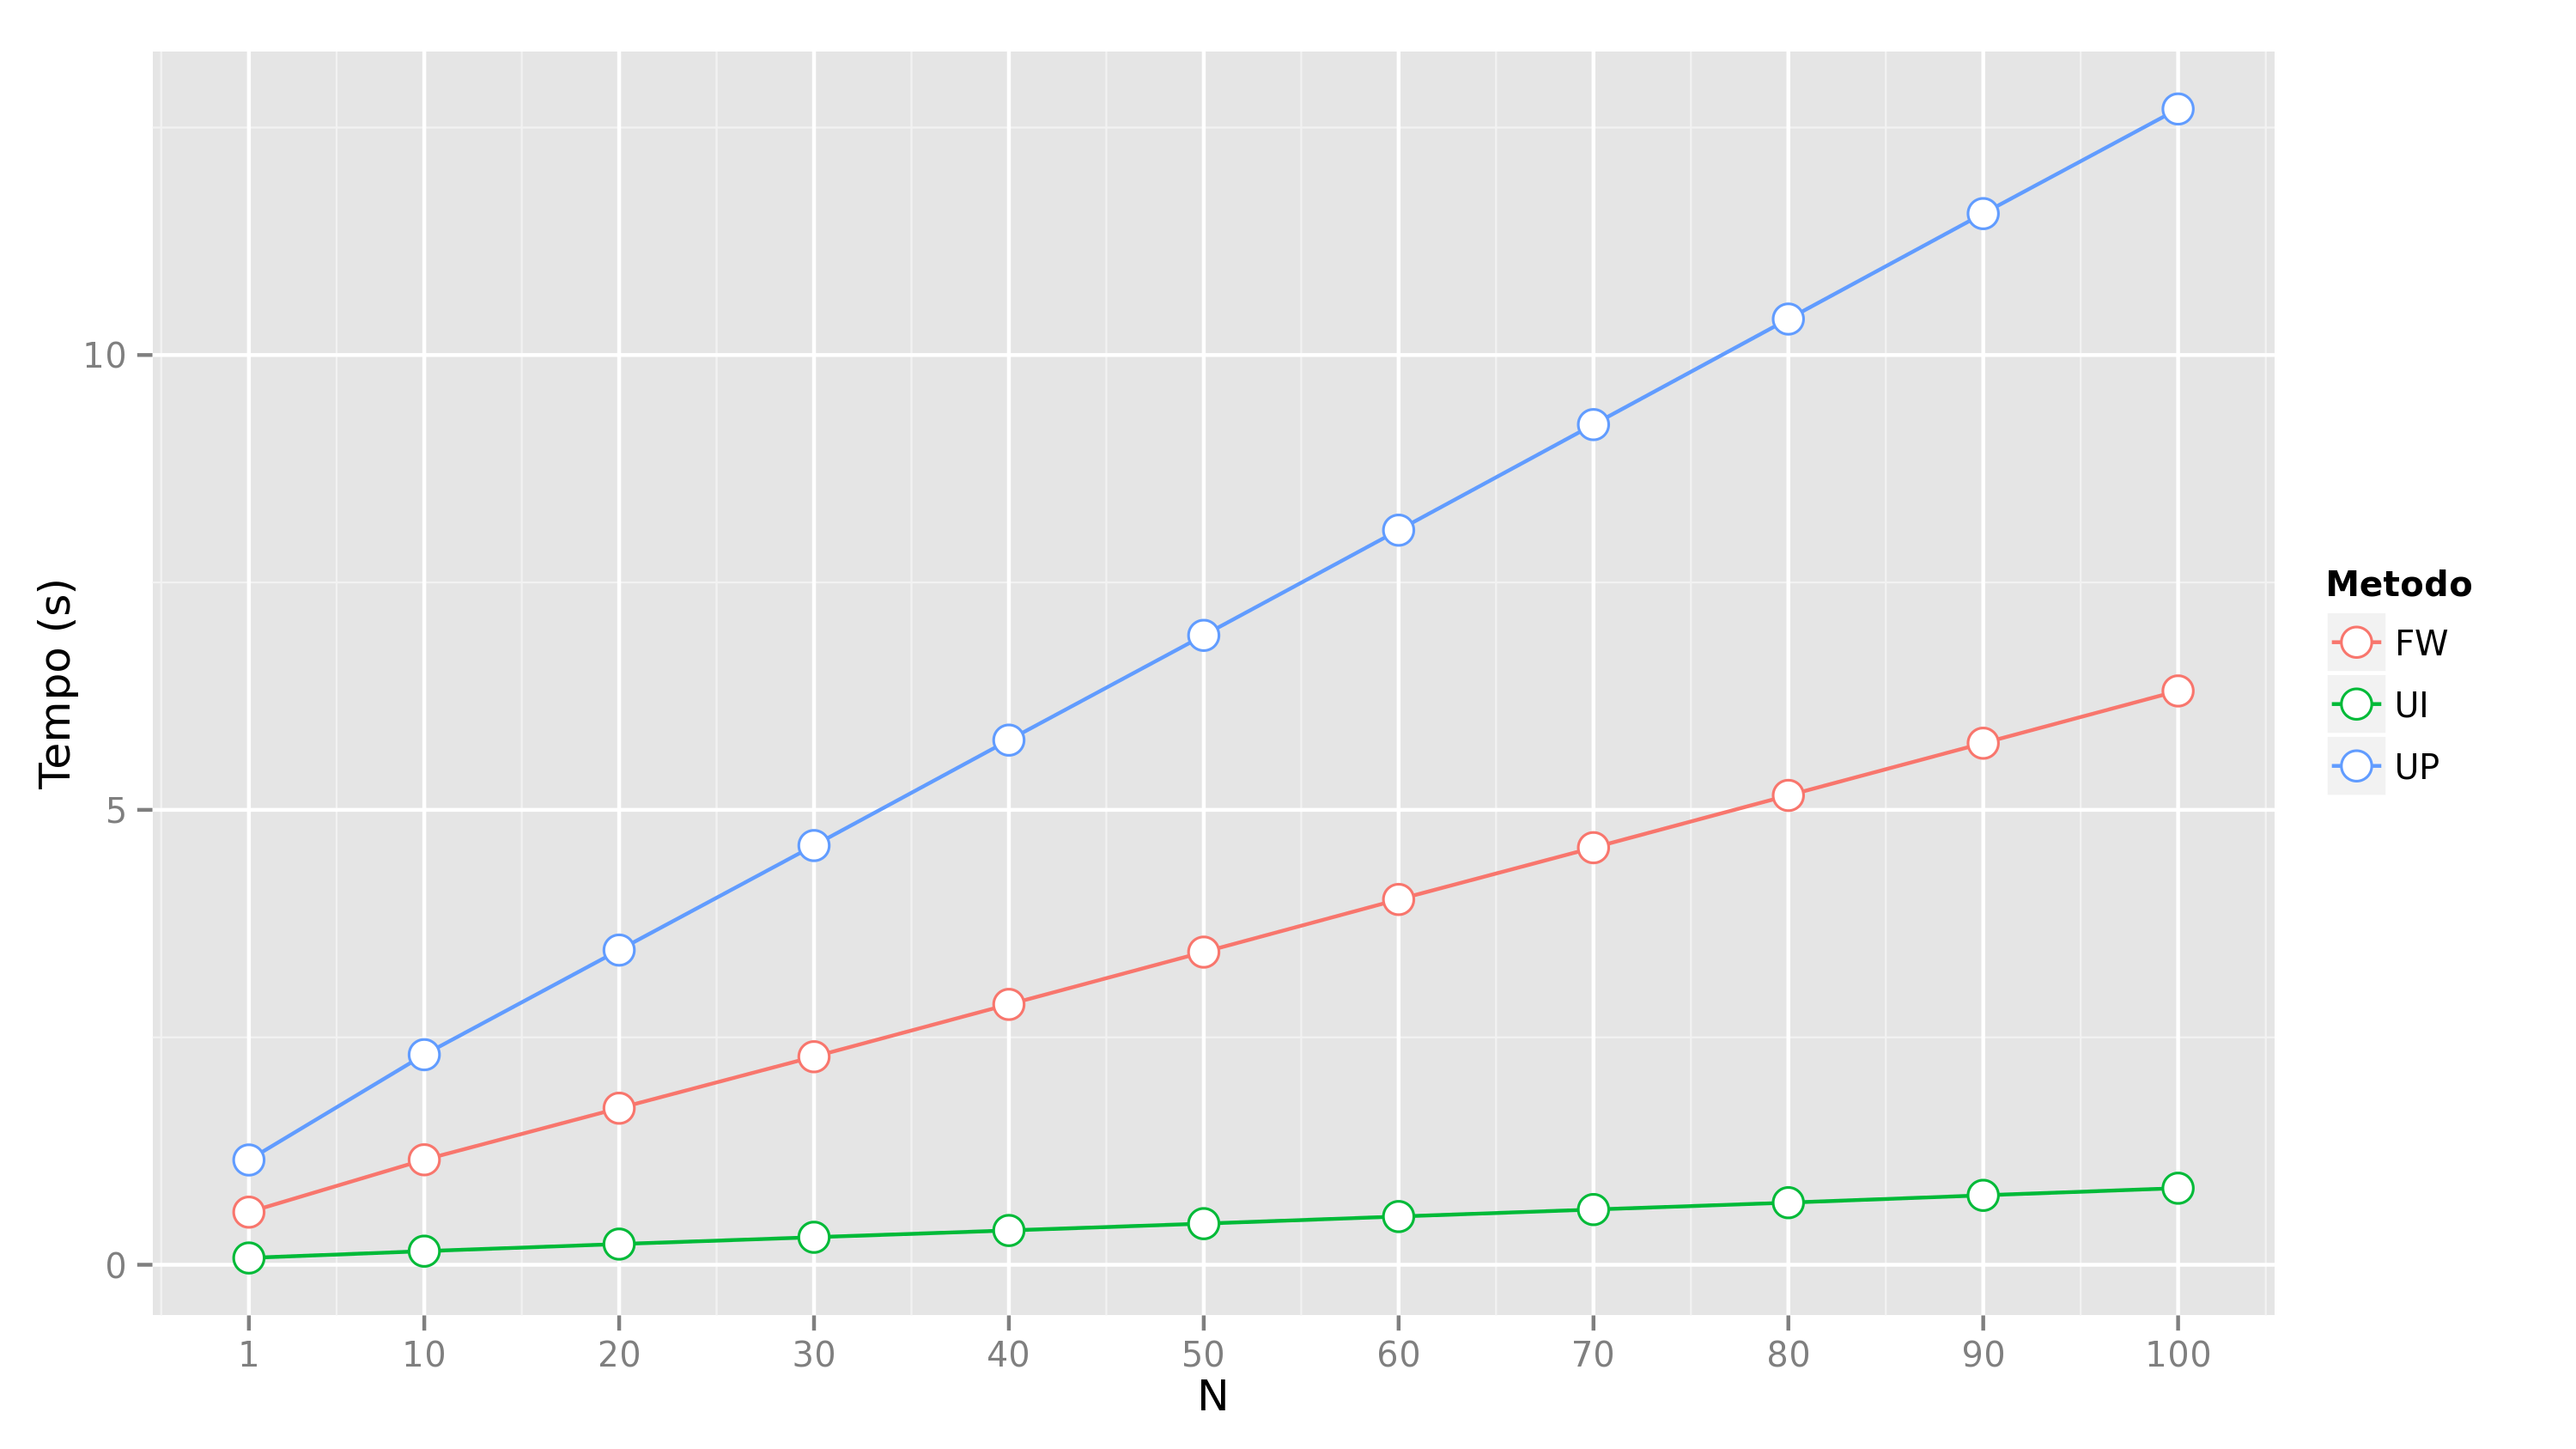
\includegraphics[width=1\textwidth]{img/time_N}
    \end{center}
    \caption{Tempo de execução em função do tamanho da lista de recomendações $N$}
    \label{fig:time_N}
\end{figure}

Contrariamente ao esperado, a qualidade de recomendação do algoritmo UI é sensivelmente inferior à do algoritmo UP. Isso se deve ao fato de a correlação usuário-item daquele método colocar ênfase no valor do atributo $a_{if}$, mesmo que esses atributos não sejam diretamente proporcionais à preferência do usuário. Esse cálculo é incoerente, por exemplo, para atributos $f=\mathrm{data}$: mesmo que o usuário tenha um elevado interesse $w_{uf}$ por filmes antigos, o valor de $a_{if}$ não leva em conta se sua preferência é por filmes da década de 1970 ou 1990. Nesse caso, o algoritmo indicaria incorretamente que filmes mais recentes são mais adequados para aquele usuário, porque possuem maior $a_{if}$.

A fim de corrigir essa falha no algoritmo UI, seria necessário, por exemplo, aplicar nos atributos $a_{if}$ uma função $g_f$ que crescesse no mesmo sentido do interesse do usuário por aquela \textit{feature}. Dessa forma, o cálculo $\sum_f w_{uf}~g_f\left(a_{if}\right)$ significaria de fato a similaridade entre o usuário $u$ e o item $i$ medida através de seu interesse $g\left(a_{if}\right)$ pelas \textit{features} $f$.

Apesar de alta qualidade das recomendações do método UP, este possui também a maior complexidade computacional. Seu tempo de execução é 2 vezes maior que o do método FW e 4 vezes maior que o do método UI. Todavia, nenhum desses tempos de execução é crítico, tendo em vista que o sistema não seria colocado diretamente à disposição dos clientes, mas que as recomendações seriam enviadas via email, por exemplo. 

Apenas o método UI atende ao requisito de \textit{throughput} mínimo de 28 recomendações para cada usuário por segundo. Dado que a base de testes possui $25\%$ do total de usuários, correspondente a 236 clientes para o banco 100k, o tempo de execução máximo dos métodos deveria ser de $0.15$ min. A fim de melhorar a velocidade das recomendações, a solução mais eficiente é a mudança da linguagem de programação. O uso de linguagens C, C++ ou Python pode melhorar o desempenho computacional em até 500 vezes \cite{benchmarkingR}. 

\section{Percentual da base de aprendizado $T$} % (fold)
\label{sec:percentual_da_base_de_aprendizado_}

A medida que o percentual da base de aprendizados aumenta, a precisão de todos os métodos cresce ligeiramente. Isso é consequência do caráter colaborativo dos algoritmos, já que a qualidade da recomendação depende da quantidade total de dados. Entretanto, pode-se observar que a abrangência e a medida $F_1$ são praticamente constantes para valores crescentes de $T$ de modo que esse parâmetro não tem grande relevância para o sucesso do sistema de recomendação.

O parâmetro $T$ não exerce nenhuma influência sobre o tempo de execução dos métodos UP e UI, mas apenas sobre o método FW. Isso ocorre porque a etapa de maior custo computacional (Equação \ref{eq:determinacao-wf}) é linearmente dependente da quantidade de usuários $\left|\mathcal{U}\right|$. Quanto menos usuários-teste, mais veloz é o algoritmo.

\begin{figure}[htp]
    \begin{center}
    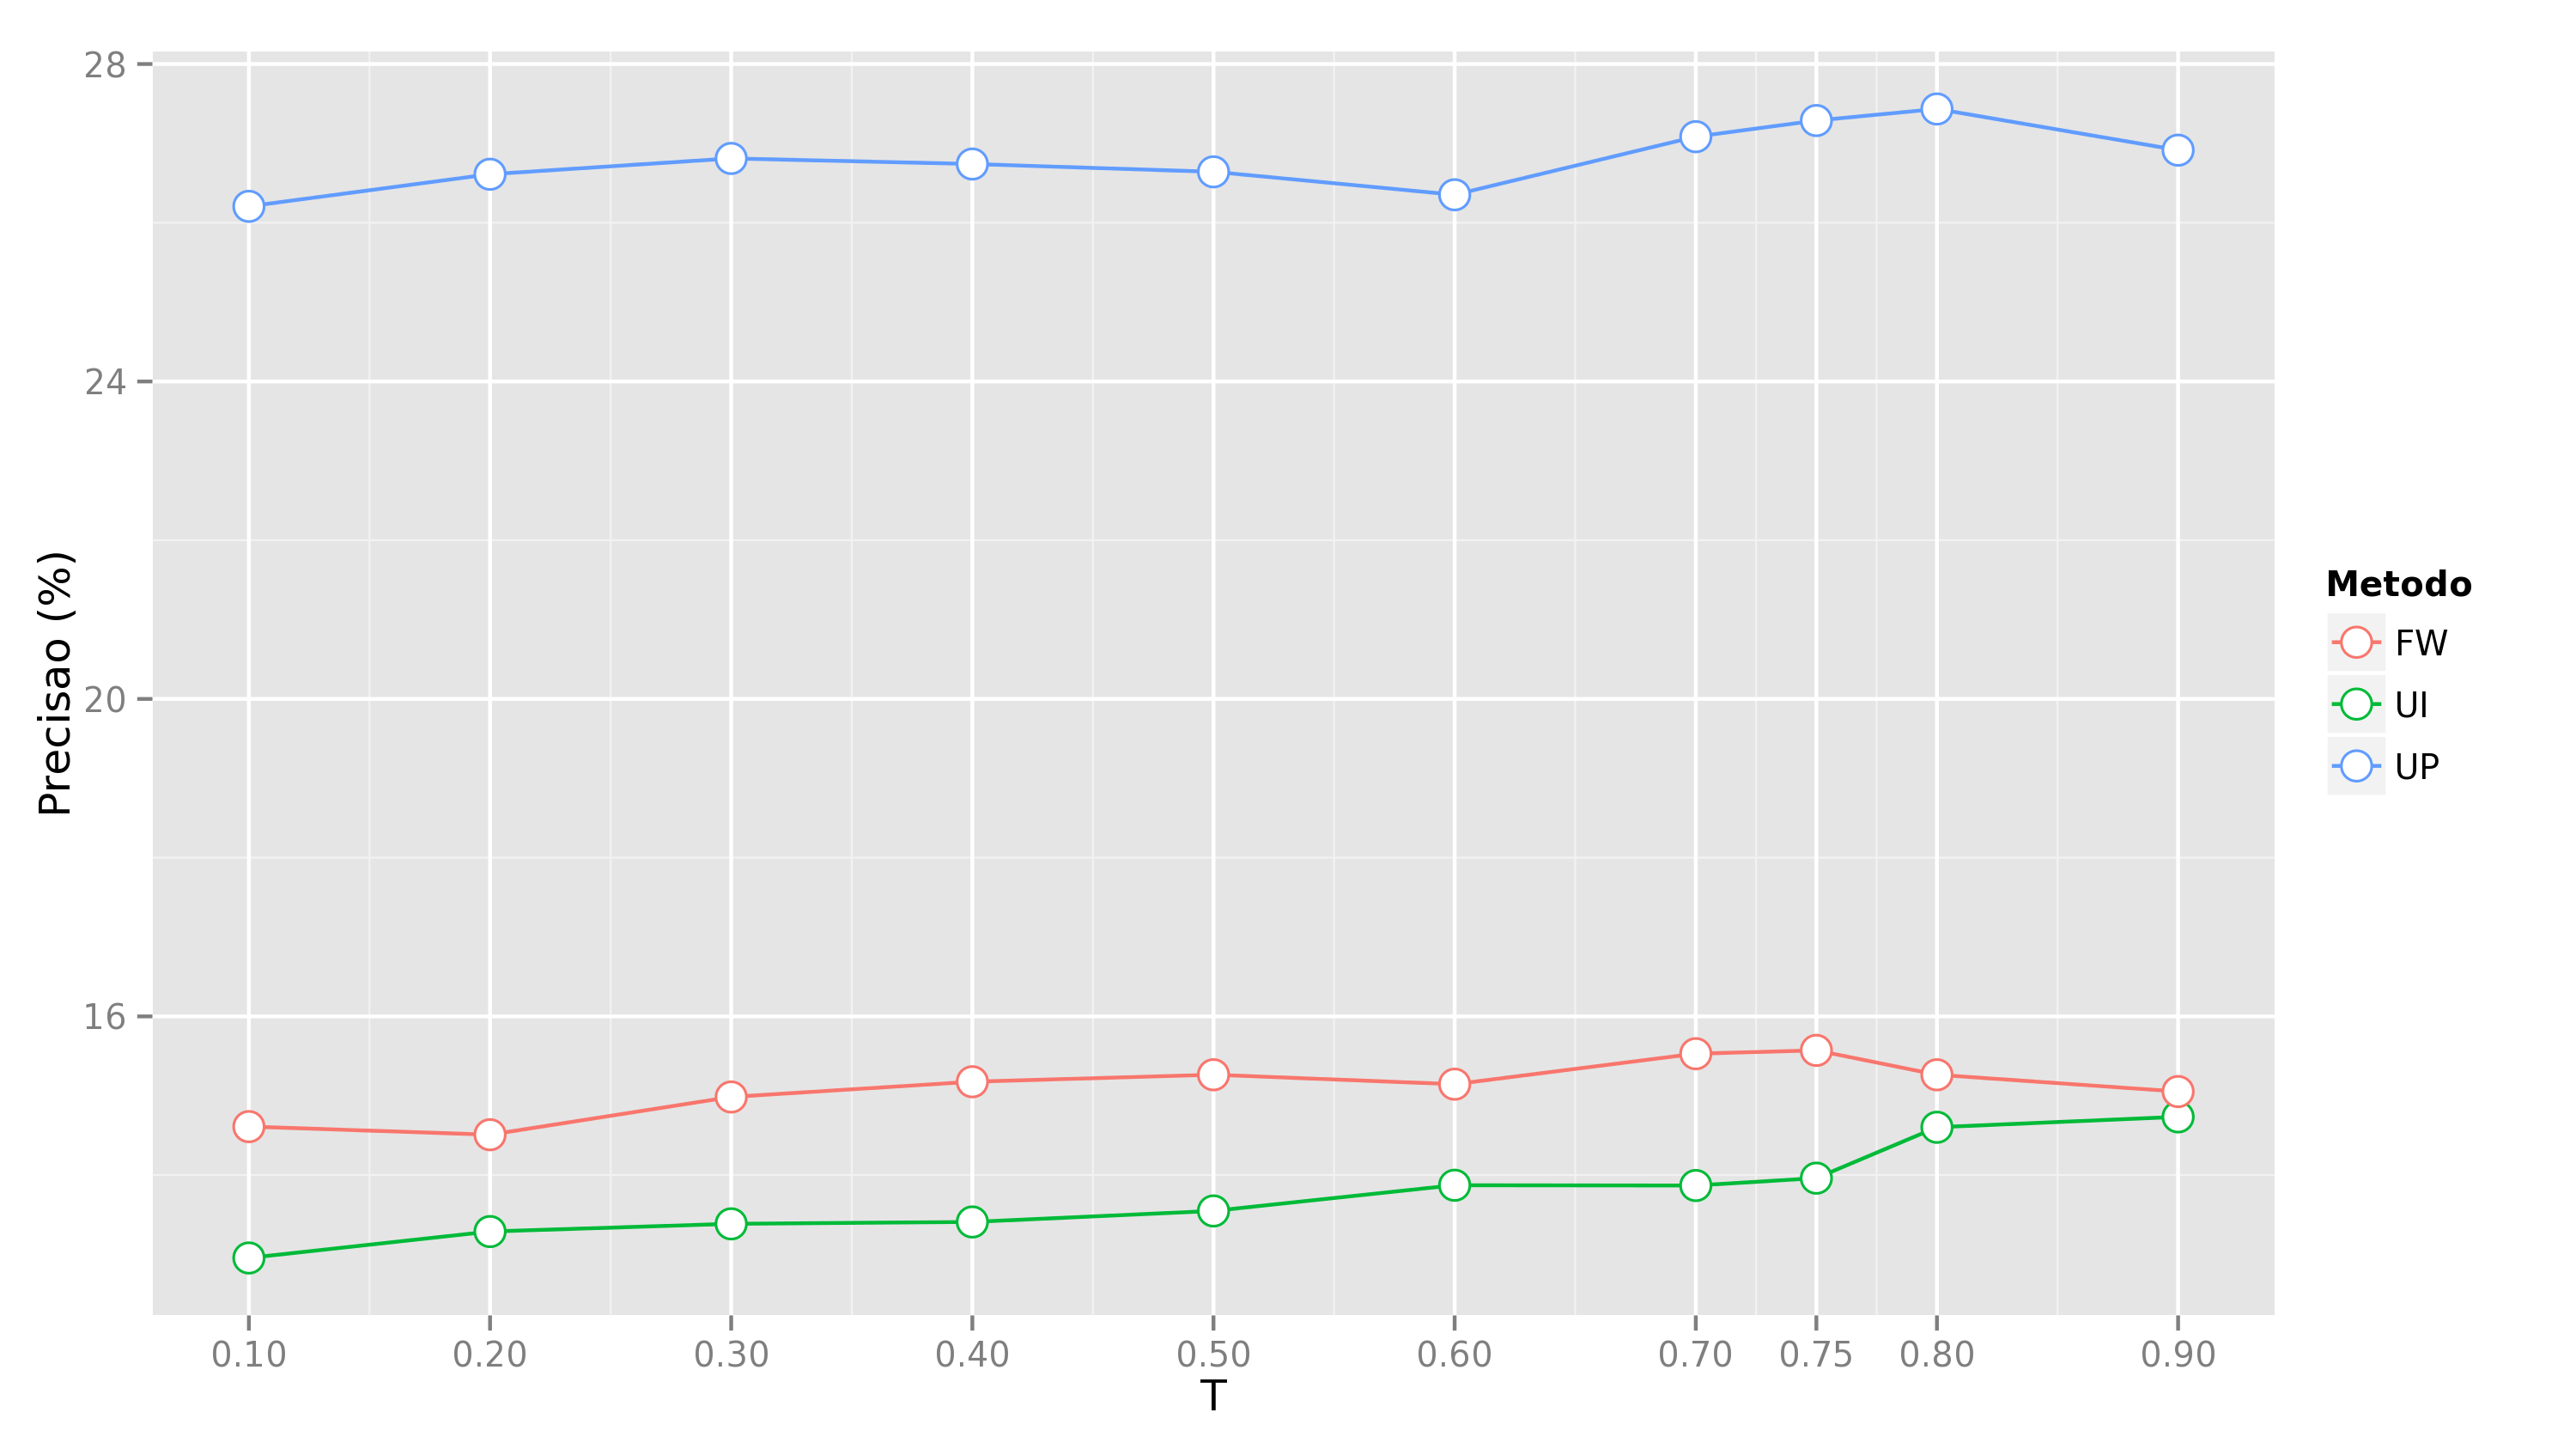
\includegraphics[width=1\textwidth]{img/precision_T}
    \end{center}
    \caption{Precisão em função do percentual da base de aprendizado $T$}
    \label{fig:precision_T}
\end{figure}


\begin{figure}[htp]
    \begin{center}
    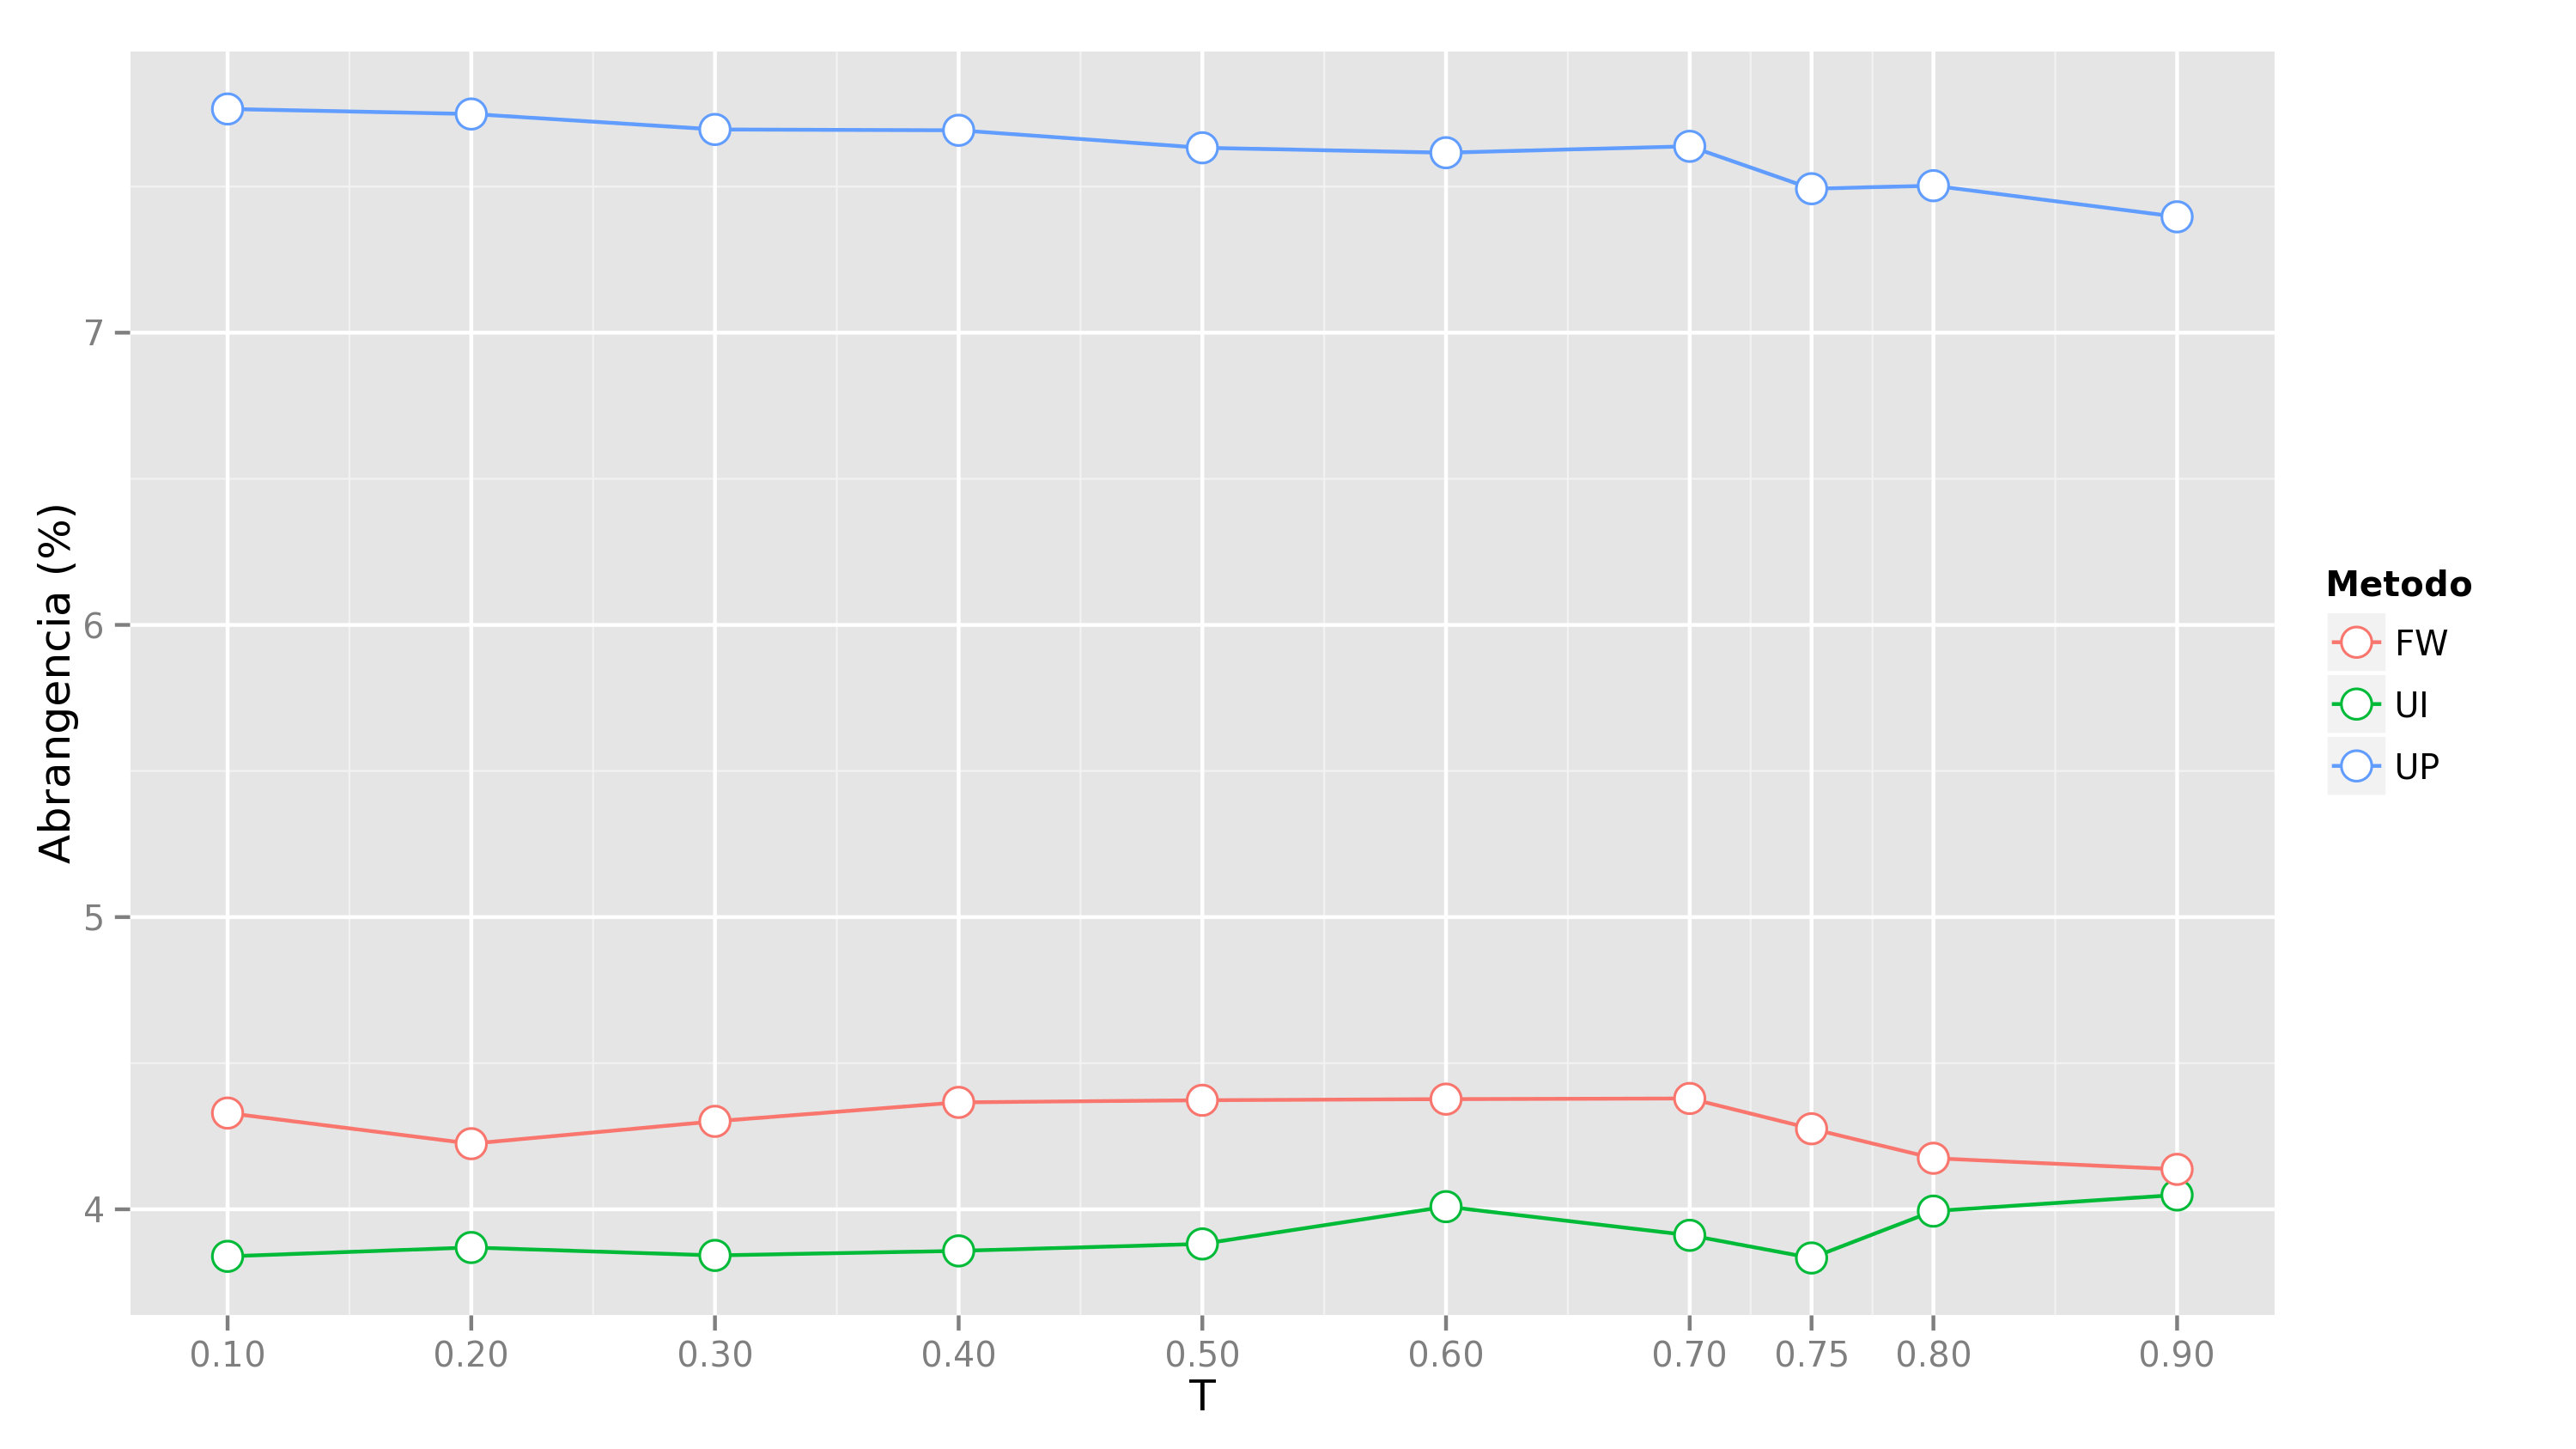
\includegraphics[width=1\textwidth]{img/recall_T}
    \end{center}
    \caption{Abrangência em função do percentual da base de aprendizado $T$}
    \label{fig:recall_T}
\end{figure}

\begin{figure}[htp]
    \begin{center}
    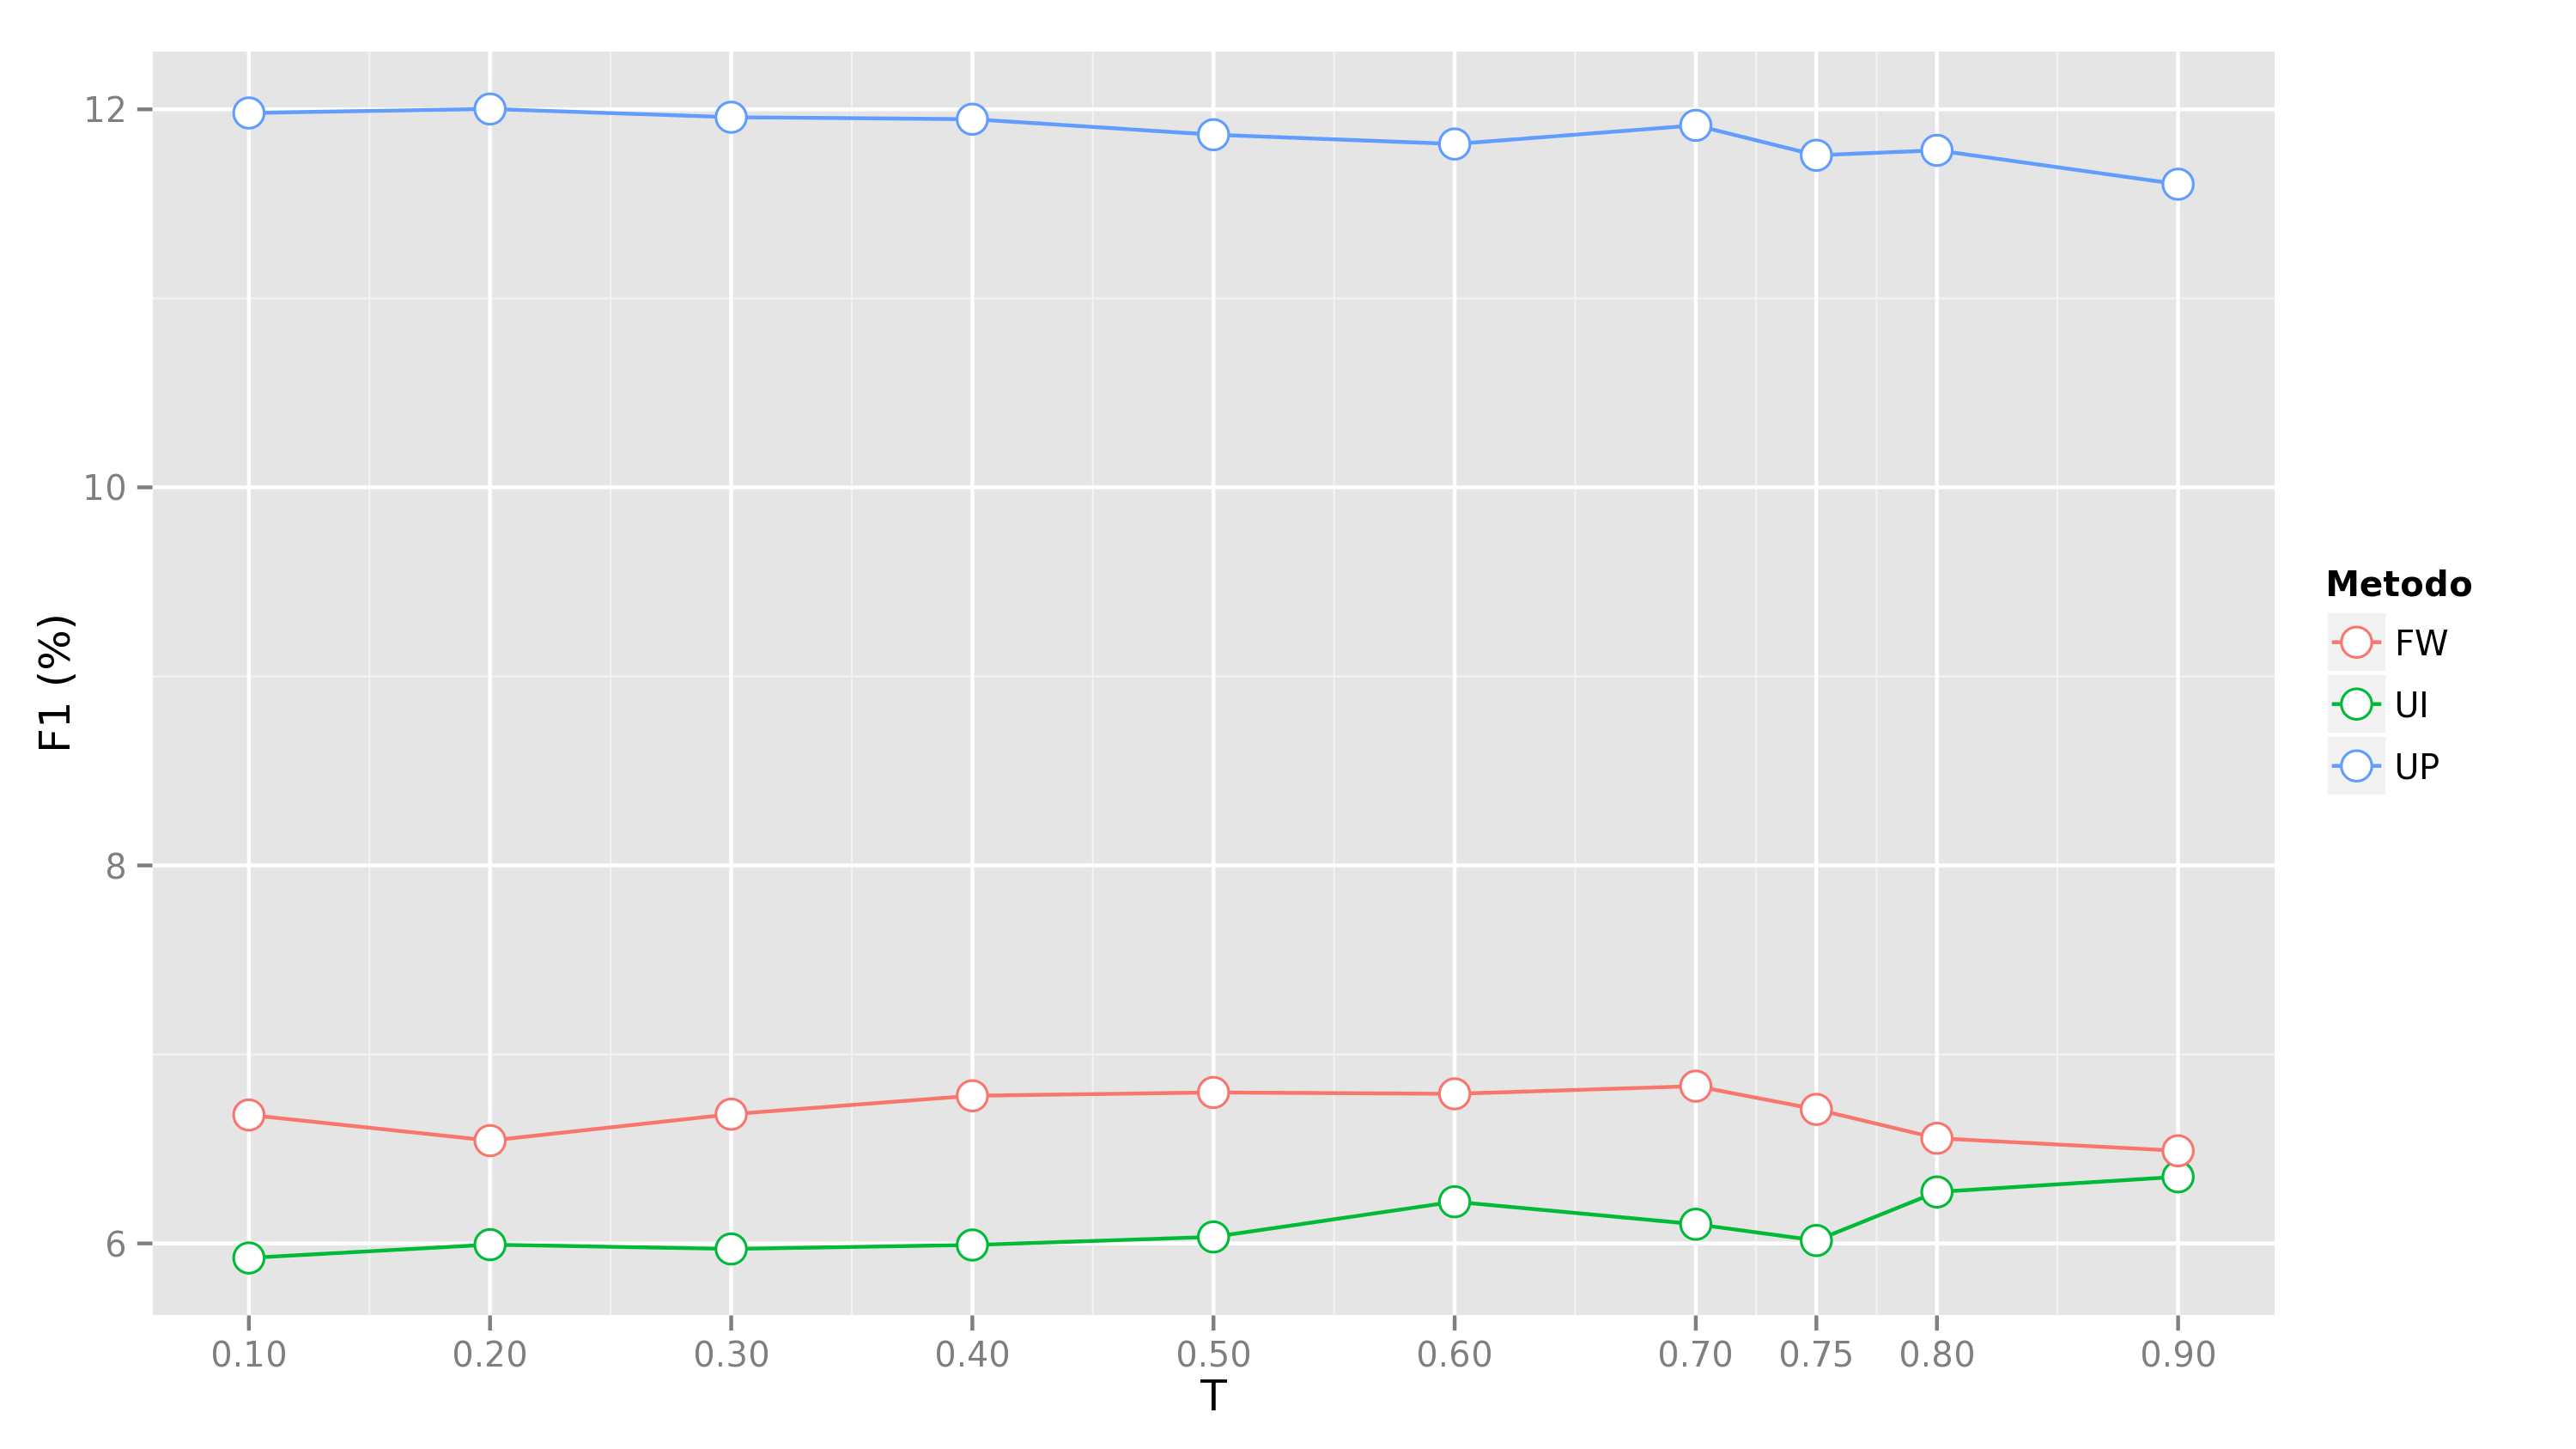
\includegraphics[width=1\textwidth]{img/F1_T}
    \end{center}
    \caption{Medida $F_1$ em função do percentual da base de aprendizado $T$}
    \label{fig:F1_T}
\end{figure}

\begin{figure}[htp]
    \begin{center}
    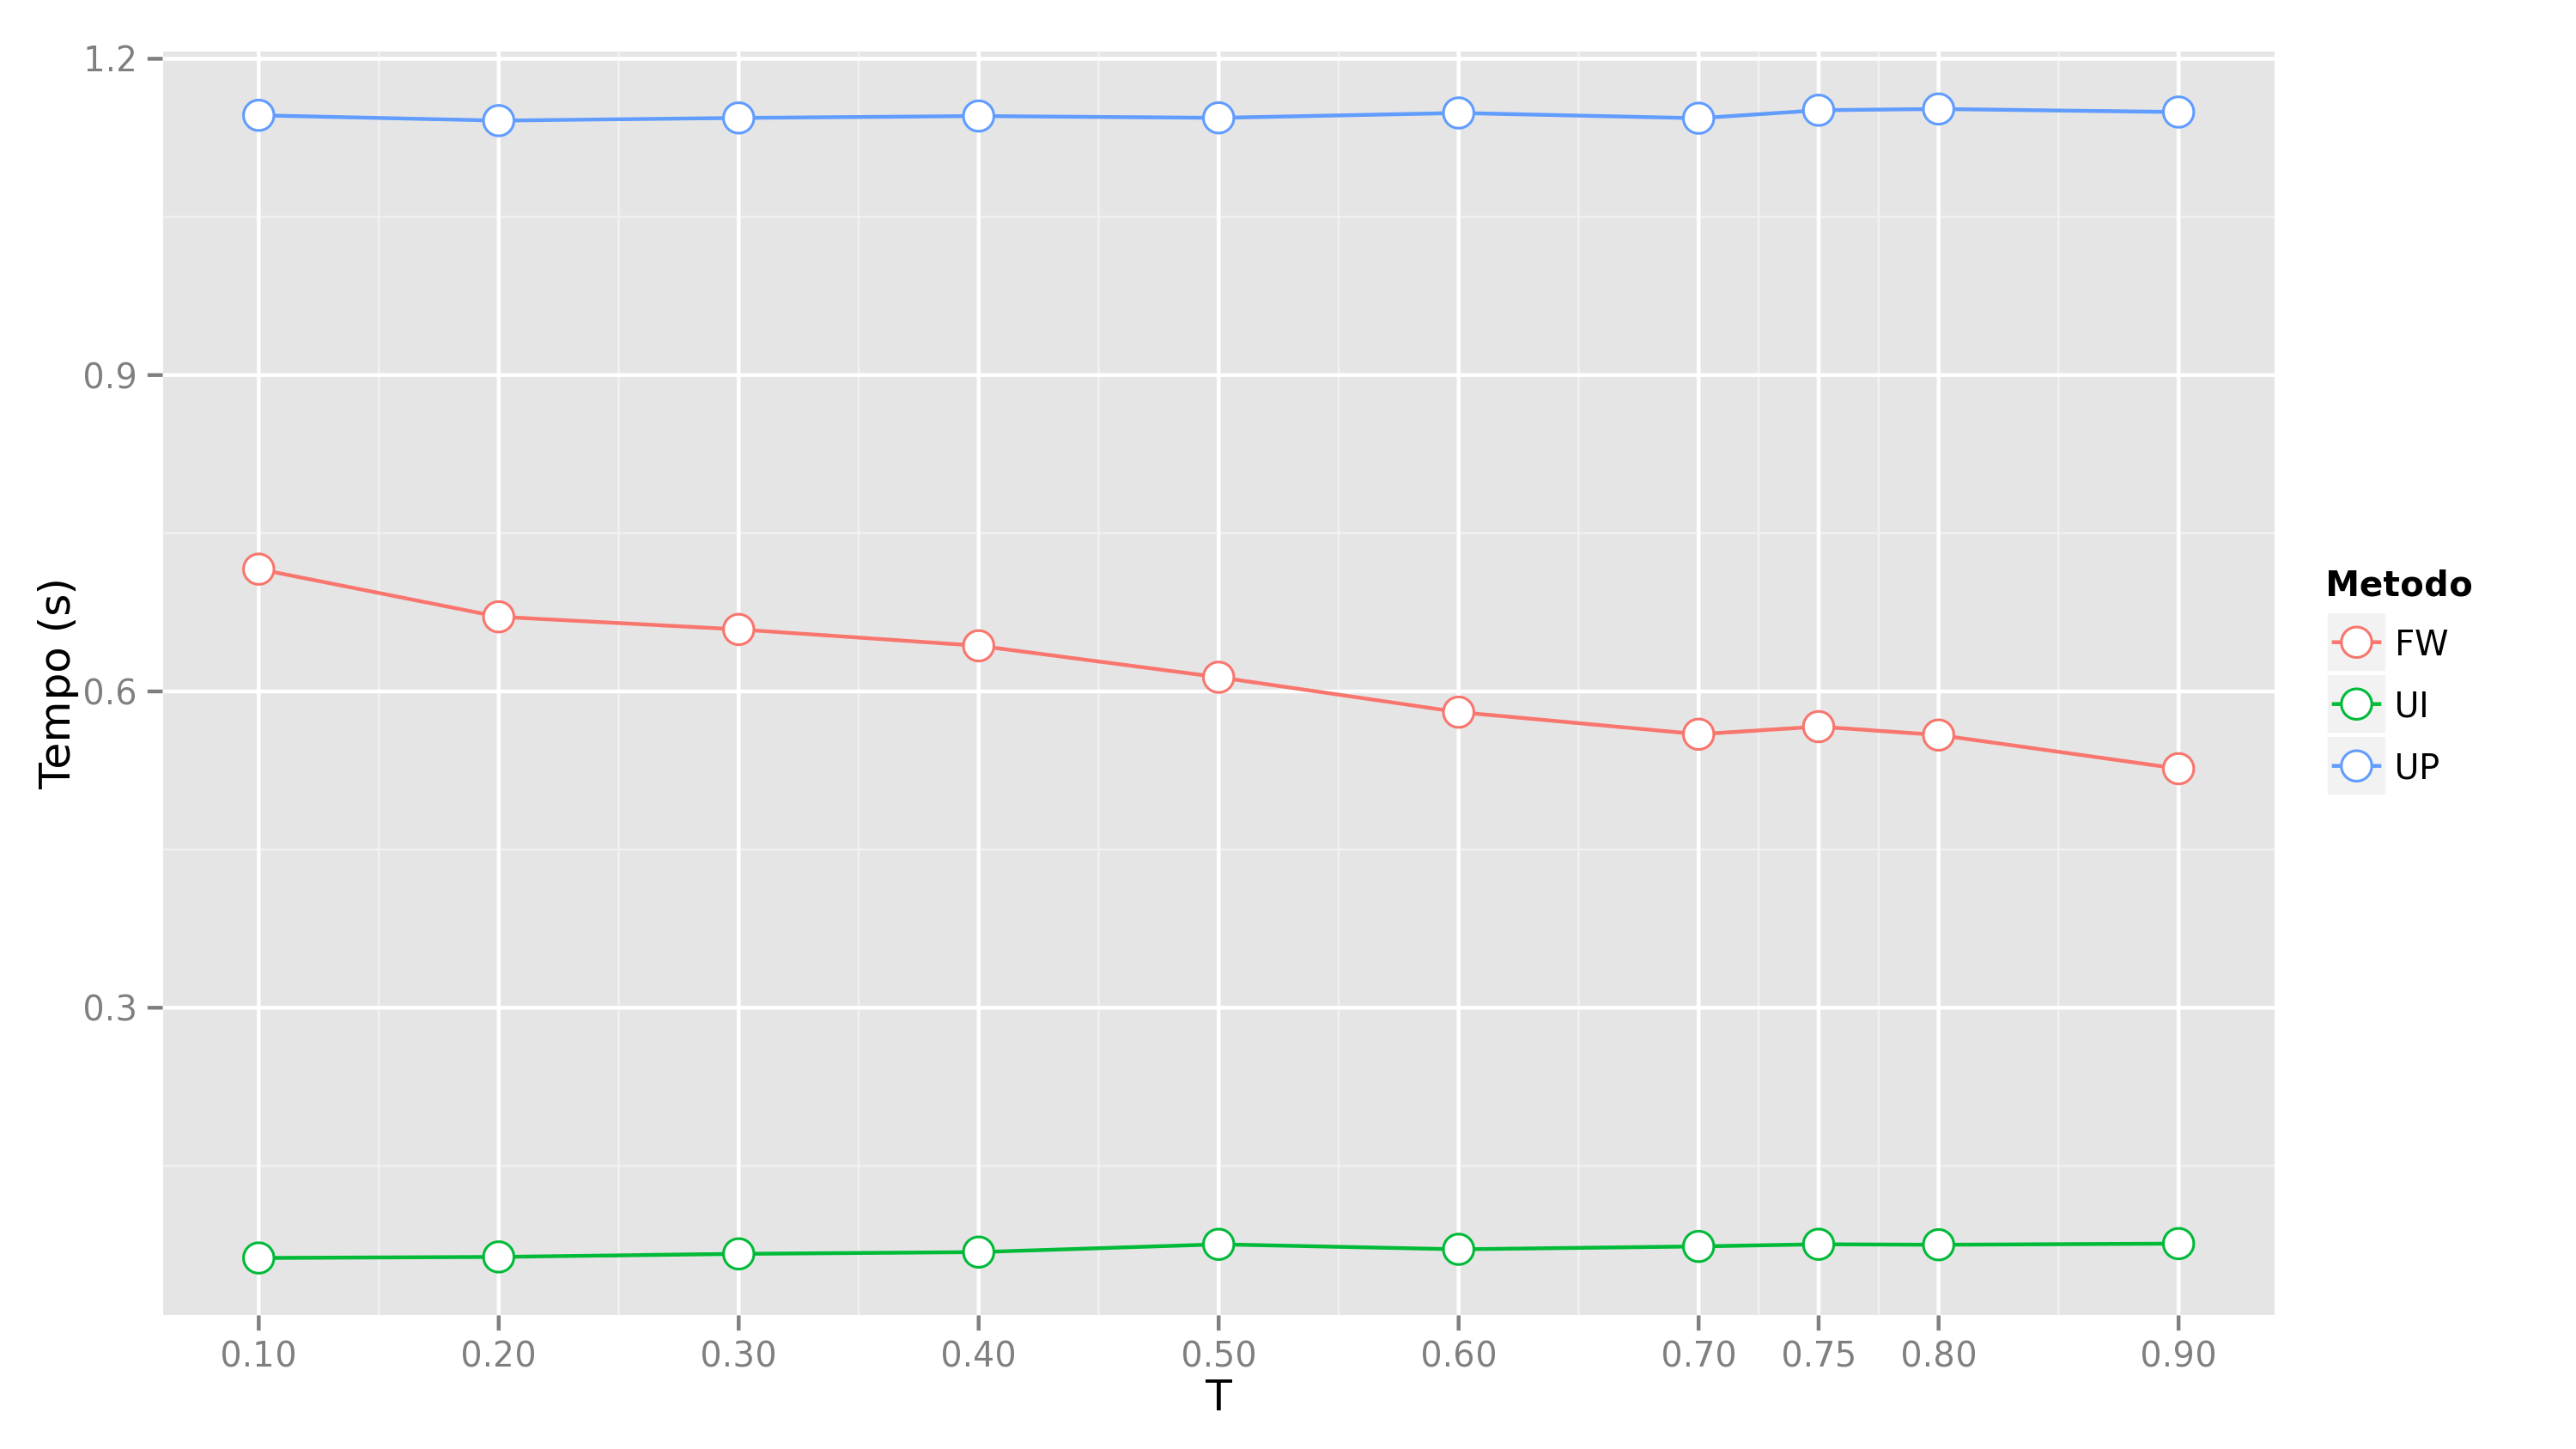
\includegraphics[width=1\textwidth]{img/time_T}
    \end{center}
    \caption{Tempo de execução em função do percentual da base de aprendizado $T$}
    \label{fig:time_T}
\end{figure}


\section{Percentual de avaliações ``escondidas'' dos usuários-teste na validação cruzada $H$} % (fold)
\label{sec:percentual_de_avalia_es_dos_usu_rios_teste_na_valida_o_cruzada}

Quanto maior o número de avaliações ``escondidas'', mais fácil é acertar os itens dos usuários-teste, pois a lista de recomendação é pequena em relação ao total de itens positivamente avaliados pelo usuário. Por esse motivo, a precisão cresce com $H$ para todos os métodos. 

Para o algoritmo FW, a precisão atinge seu máximo em $H=75\%$ e depois decresce ligeiramente (Figura \ref{fig:precision_H}). Isso ocorre porque o cálculo dos pesos $w_f$ depende da quantidade de avaliações $r_{ui}$. Existe, pois, um compromisso (\textit{tradeoff}) entre facilidade de se acertar itens avaliados quando há muitas avaliações escondidas e a dificuldade de se estimar $w_f$ quando não há muitos dados de avaliações.  

Ao passo que a precisão dos métodos aumenta com $H$, a abrangência diminui. Visto que a quantidade de itens da lista \textit{top-}$N$ é fixa, quanto maior o número de itens ``escondidos'', mais difícil é de se retornar todos os itens relevantes.

O resultado de uma precisão crescente em função de $H$ e uma acurácia decrescente é que a medida $F_1$ possui um ponto de máximo. Para todos os métodos, o valor máximo é tal que $H=50\%$.

Quanto ao tempo de execução, a influência é a mesma do parâmetro $T$: 
para o método FW, a etapa de maior custo computacional (Equação \ref{eq:determinacao-wf}) é linearmente dependente da quantidade de itens $\left|\mathcal{I}\right|$. Quanto menos avaliações de itens dos usuários-teste, mais veloz é o algoritmo.


\begin{figure}[htp]
    \begin{center}
    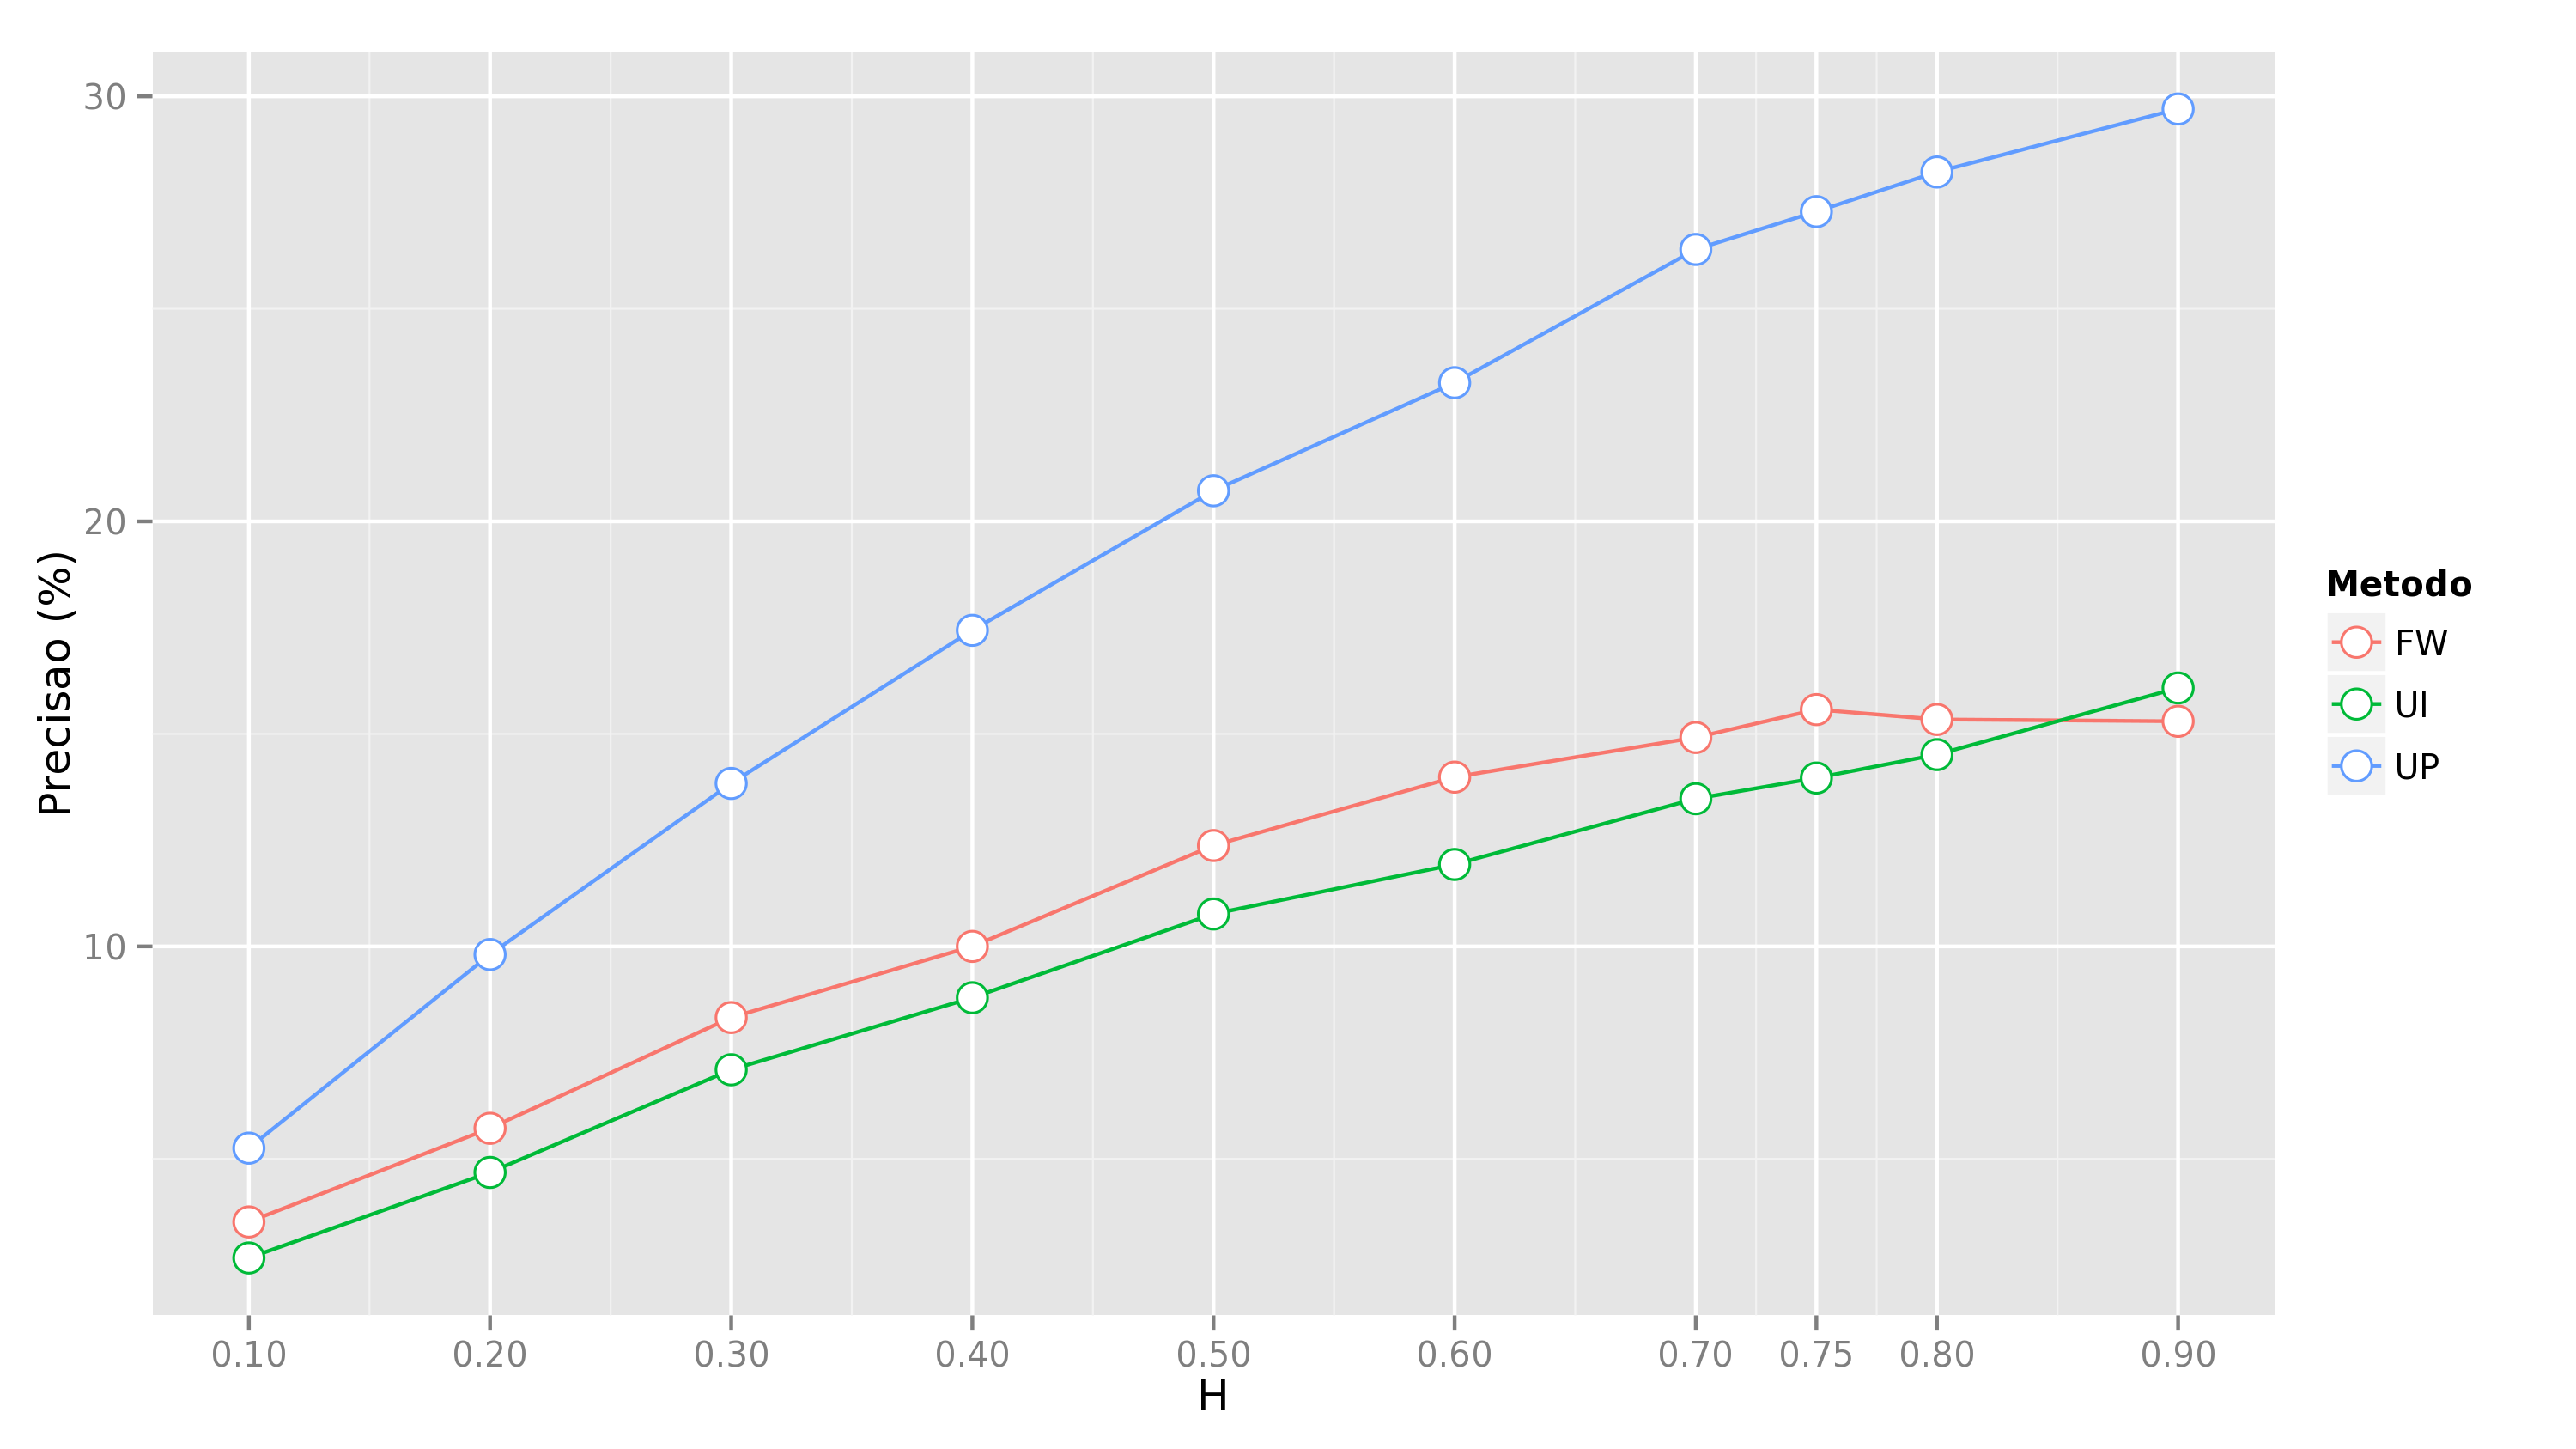
\includegraphics[width=1\textwidth]{img/precision_H}
    \end{center}
    \caption{Precisão em função do percentual de avaliações ``escondidas'' $H$}
    \label{fig:precision_H}
\end{figure}


\begin{figure}[htp]
    \begin{center}
    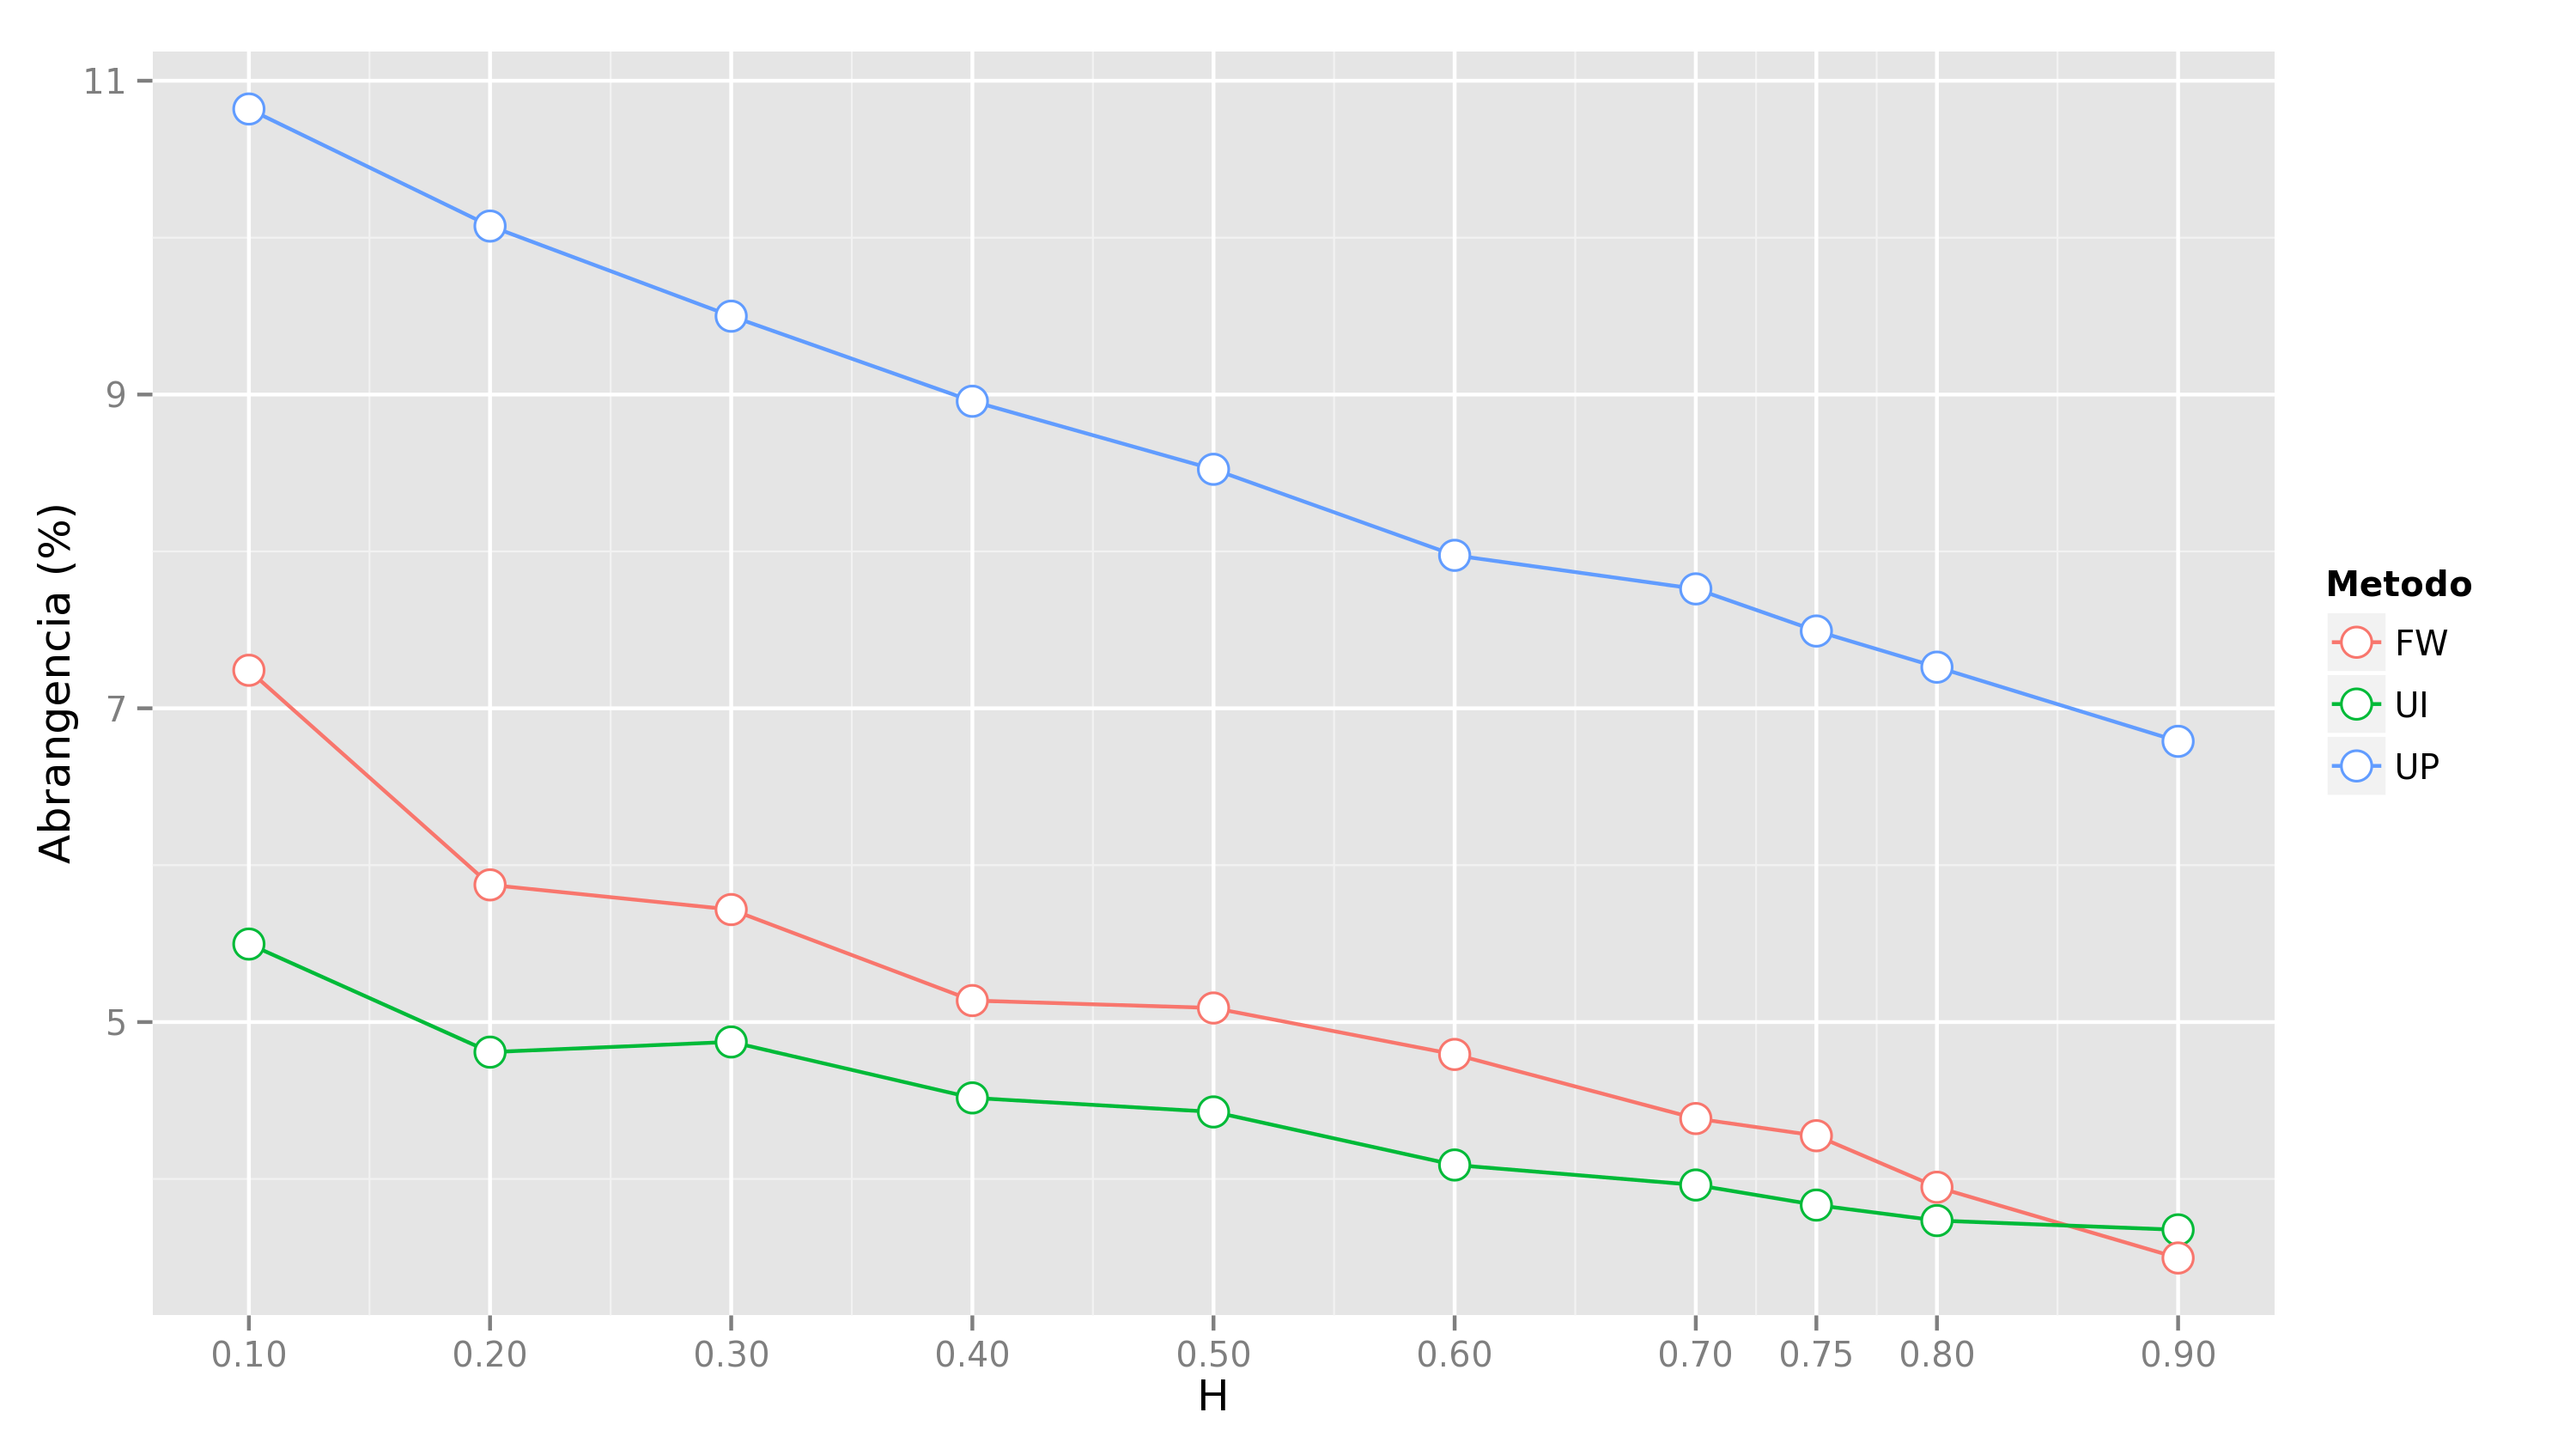
\includegraphics[width=1\textwidth]{img/recall_H}
    \end{center}
    \caption{Abrangência em função do percentual de avaliações ``escondidas'' $H$}
    \label{fig:recall_H}
\end{figure}

\begin{figure}[htp]
    \begin{center}
    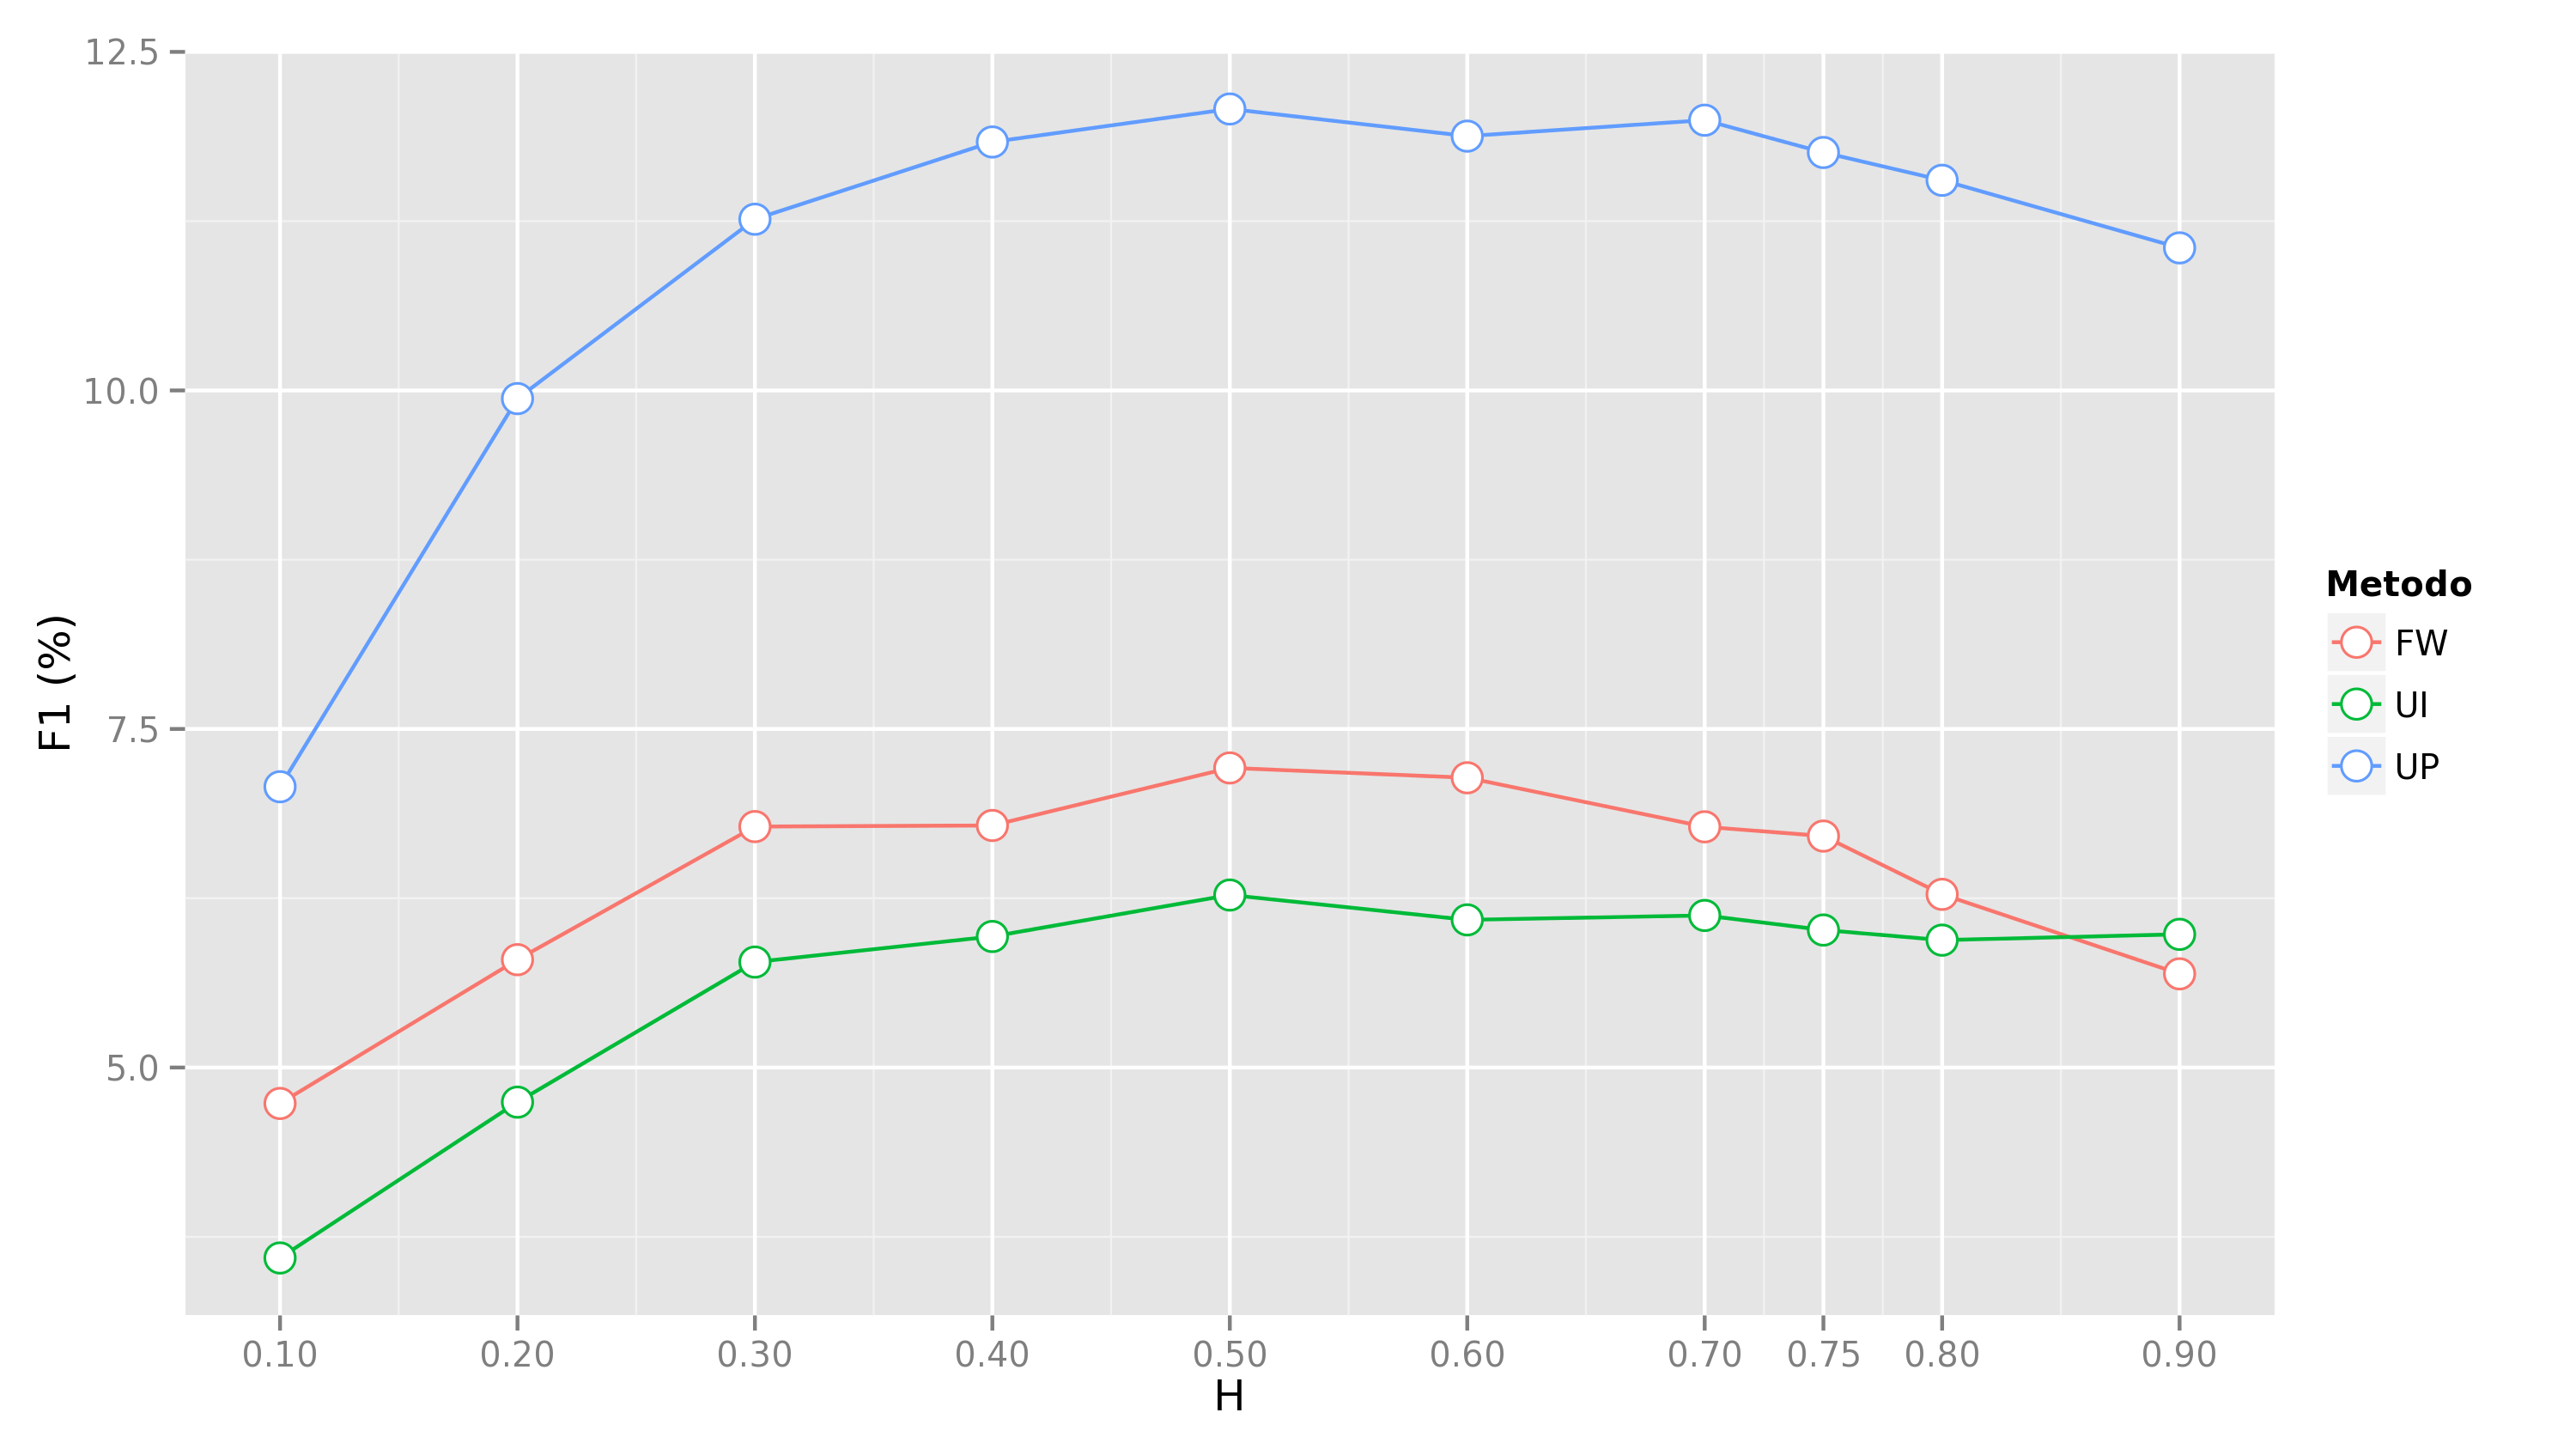
\includegraphics[width=1\textwidth]{img/F1_H}
    \end{center}
    \caption{Medida $F_1$ em função do percentual de avaliações ``escondidas'' $H$}
    \label{fig:F1_H}
\end{figure}

\begin{figure}[htp]
    \begin{center}
    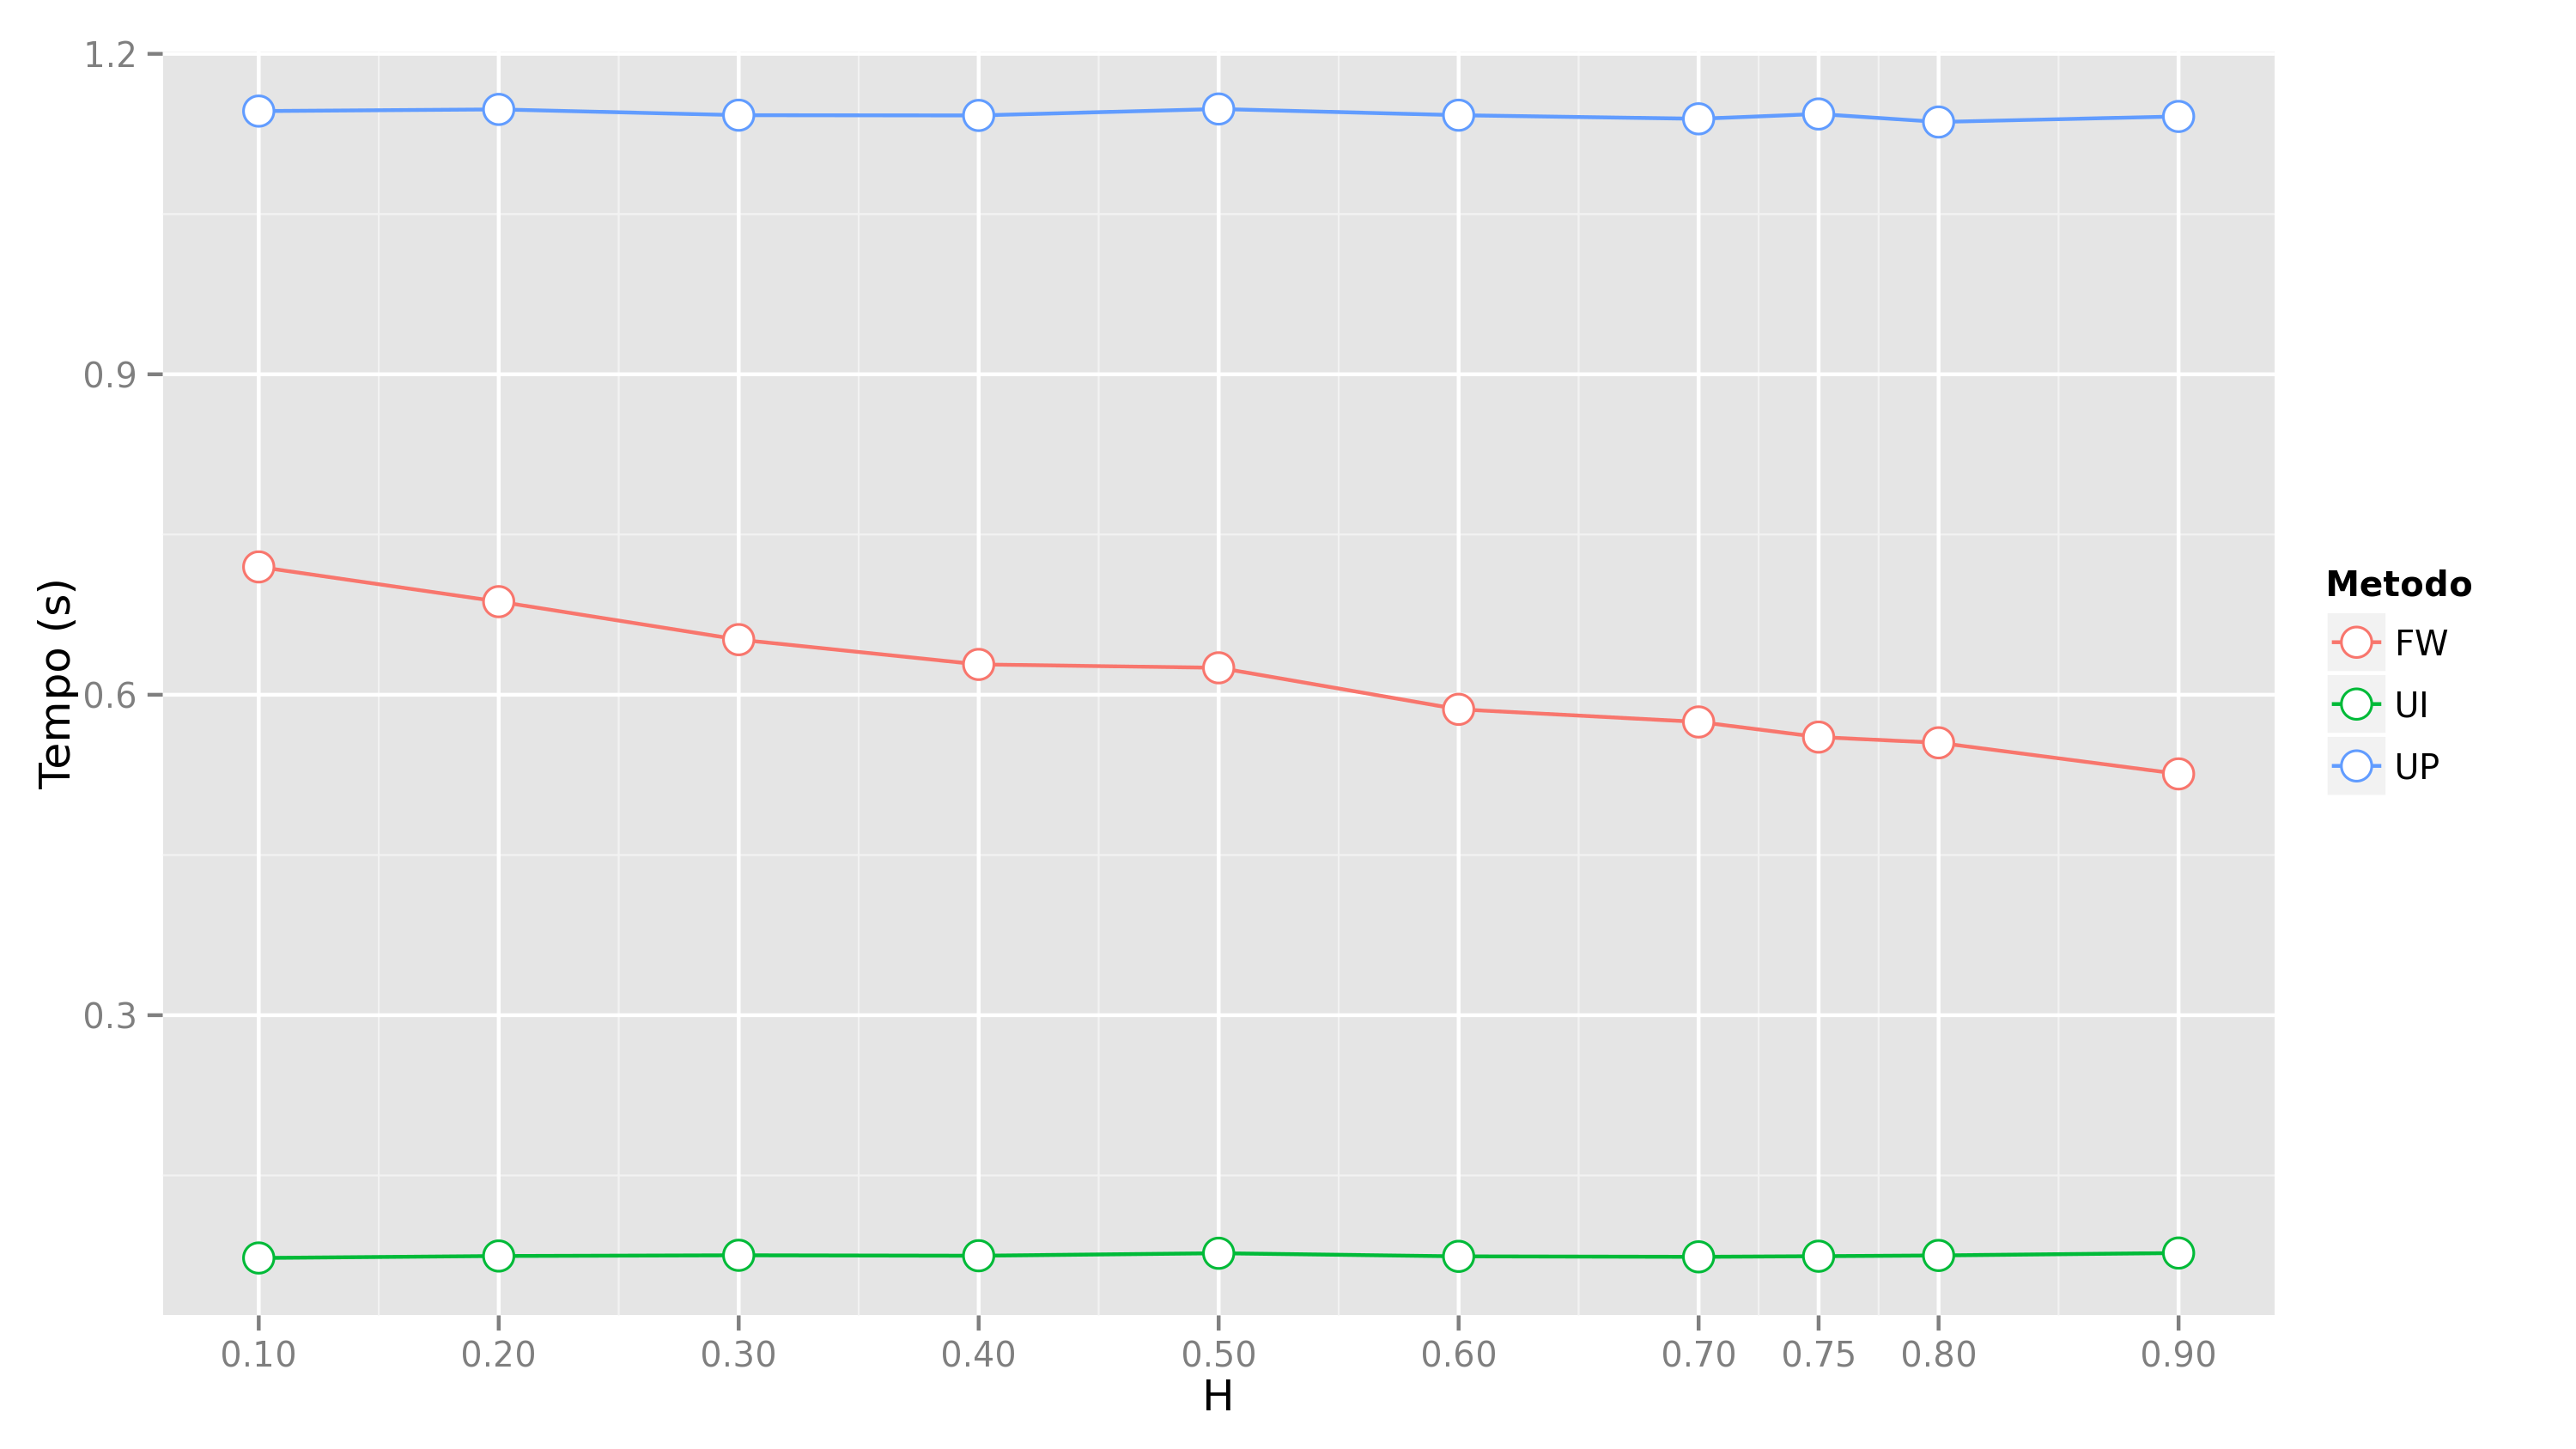
\includegraphics[width=1\textwidth]{img/time_H}
    \end{center}
    \caption{Tempo de execução em função do percentual de avaliações ``escondidas'' $H$}
    \label{fig:time_H}
\end{figure}


\section{Valor mínimo para avaliações positivas $M$} % (fold)
\label{sec:valor_m_nimo_para_avalia_es_positivas_}

Contrariamente ao que esperávamos, tornar o algoritmo mais ``seletivo'' não melhora sua precisão. Apesar de o valor mínimo $M$ estar intimamente ligado com a noção de ``avaliação positiva'' e de entrar no cálculo de parâmetros importantes dos métodos (Equações \ref{eq:determinacao-eij} e \ref{eq:tf}), esse parâmetro pouco influencia a precisão para $0 \leq M \leq 2$. 

Esse resultado pode ser explicado pelo fato de que a maioria das avaliações são positivas (Figura \ref{fig:percentual_M}), e portanto $\mathrm{b}_M$ tem quase o mesmo efeito de $\mathrm{b}_0$. Isso não ocorre somente pelo fato de os clientes comprarem itens similares a seus gostos, e portanto de raramente se decepcionarem, mas também pelo fato de que os usuários tem menos disposição para darem avaliações negativas. Esse fenômeno se chama \textit{hidden feedback}, e se caracteriza pelo fato de que os itens avaliados não são escolhidos ao acaso, mas sim por despertarem aspectos de interesse das preferências do usuário, indo além dos valores numéricos das avaliações \cite{lops2011content-chap5}.

Ao se analisar a abrangência dos métodos, a seletividade influencia na recomendação. Quanto maior $M$, menor é a quantidade de itens muito bem avaliados. Estes possuem elevada similaridade-correlação e são facilmente escolhidos pelos algoritmos. Por esse motivo, melhor é o desempenho do sistema.

A complexidade computacional dos algoritmos também depende de $M$, já que mais ou menos parâmetros são analisados no cálculo da TF-IDF (métodos UI e UP) e dos pesos dos atributos (método FW).

Um detalhe a se observar é que a precisão é nula e a abrangência é inexistente para $M=5$, já que todas as avaliações $r_{ui}$ pertencem ao conjunto $\left\{1,2,3,4,5\right\}$. 
Para o algoritmo UI, tanto a precisão quanto a abrangência são nulas para $M=4$.

\begin{figure}[htp]
    \begin{center}
    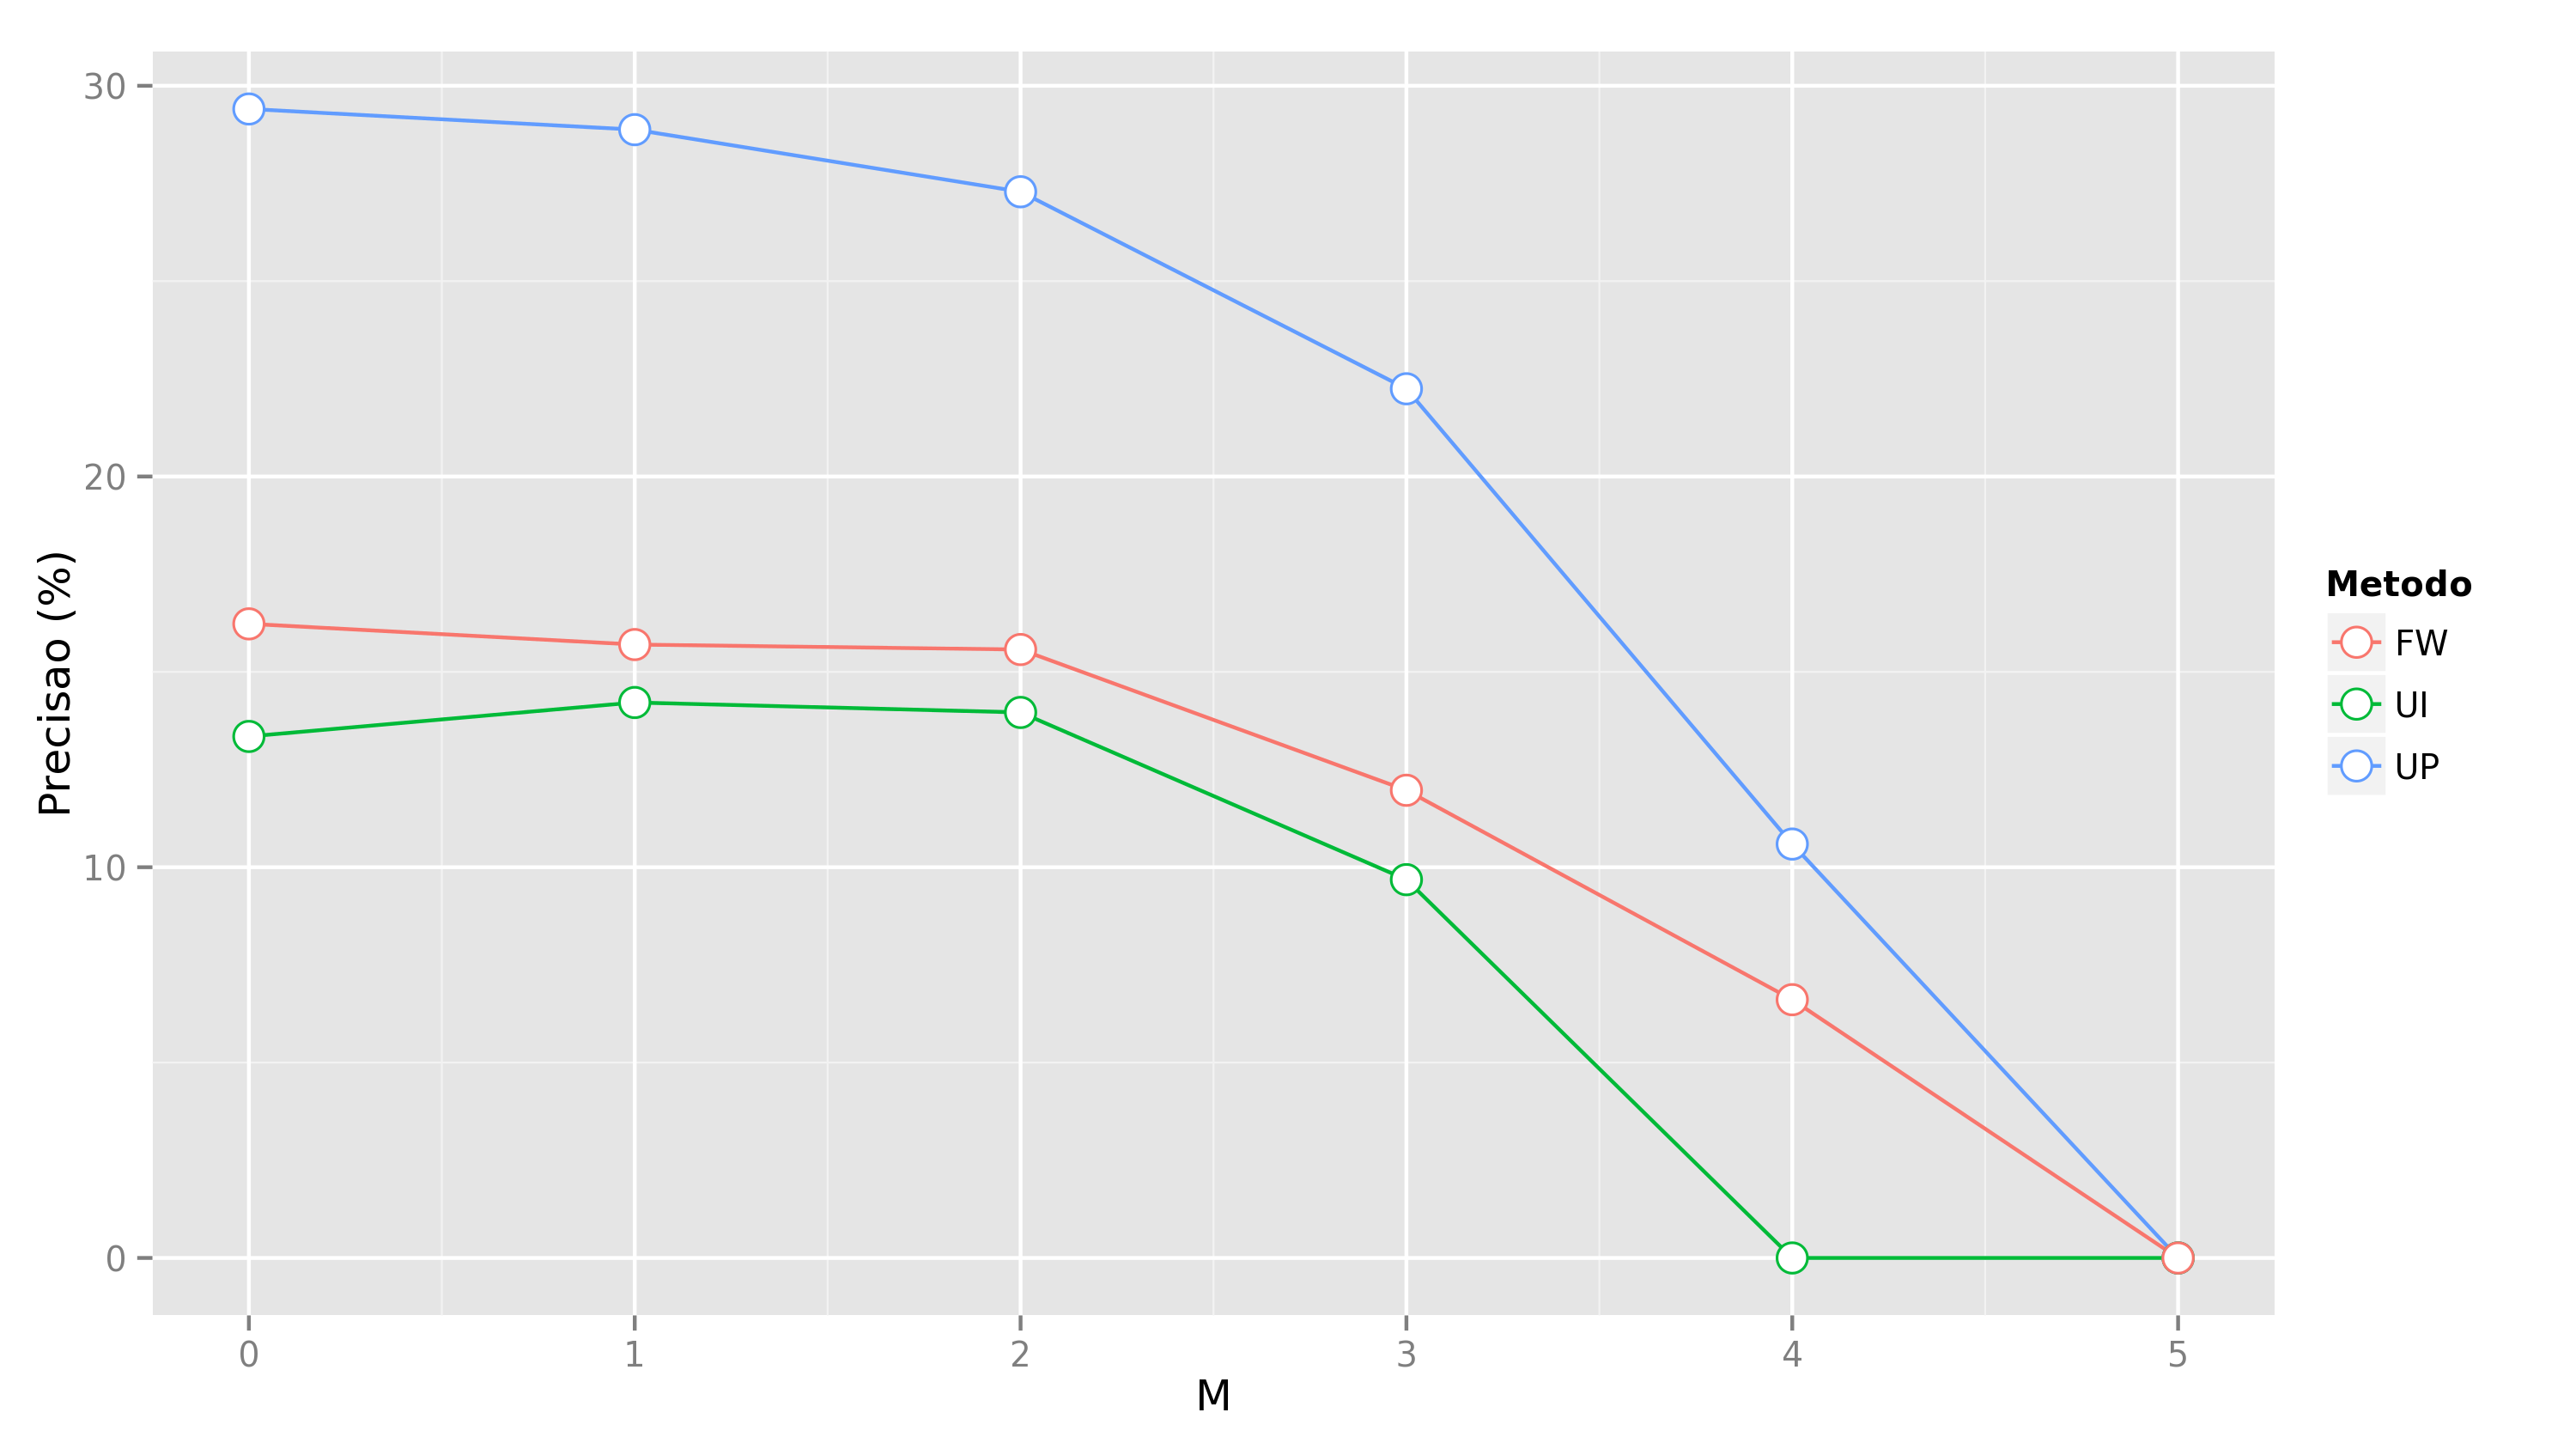
\includegraphics[width=1\textwidth]{img/precision_M}
    \end{center}
    \caption{Precisão em função do valor mínimo para avaliações positivas $M$}
    \label{fig:precision_M}
\end{figure}

\begin{figure}[htp]
    \begin{center}
    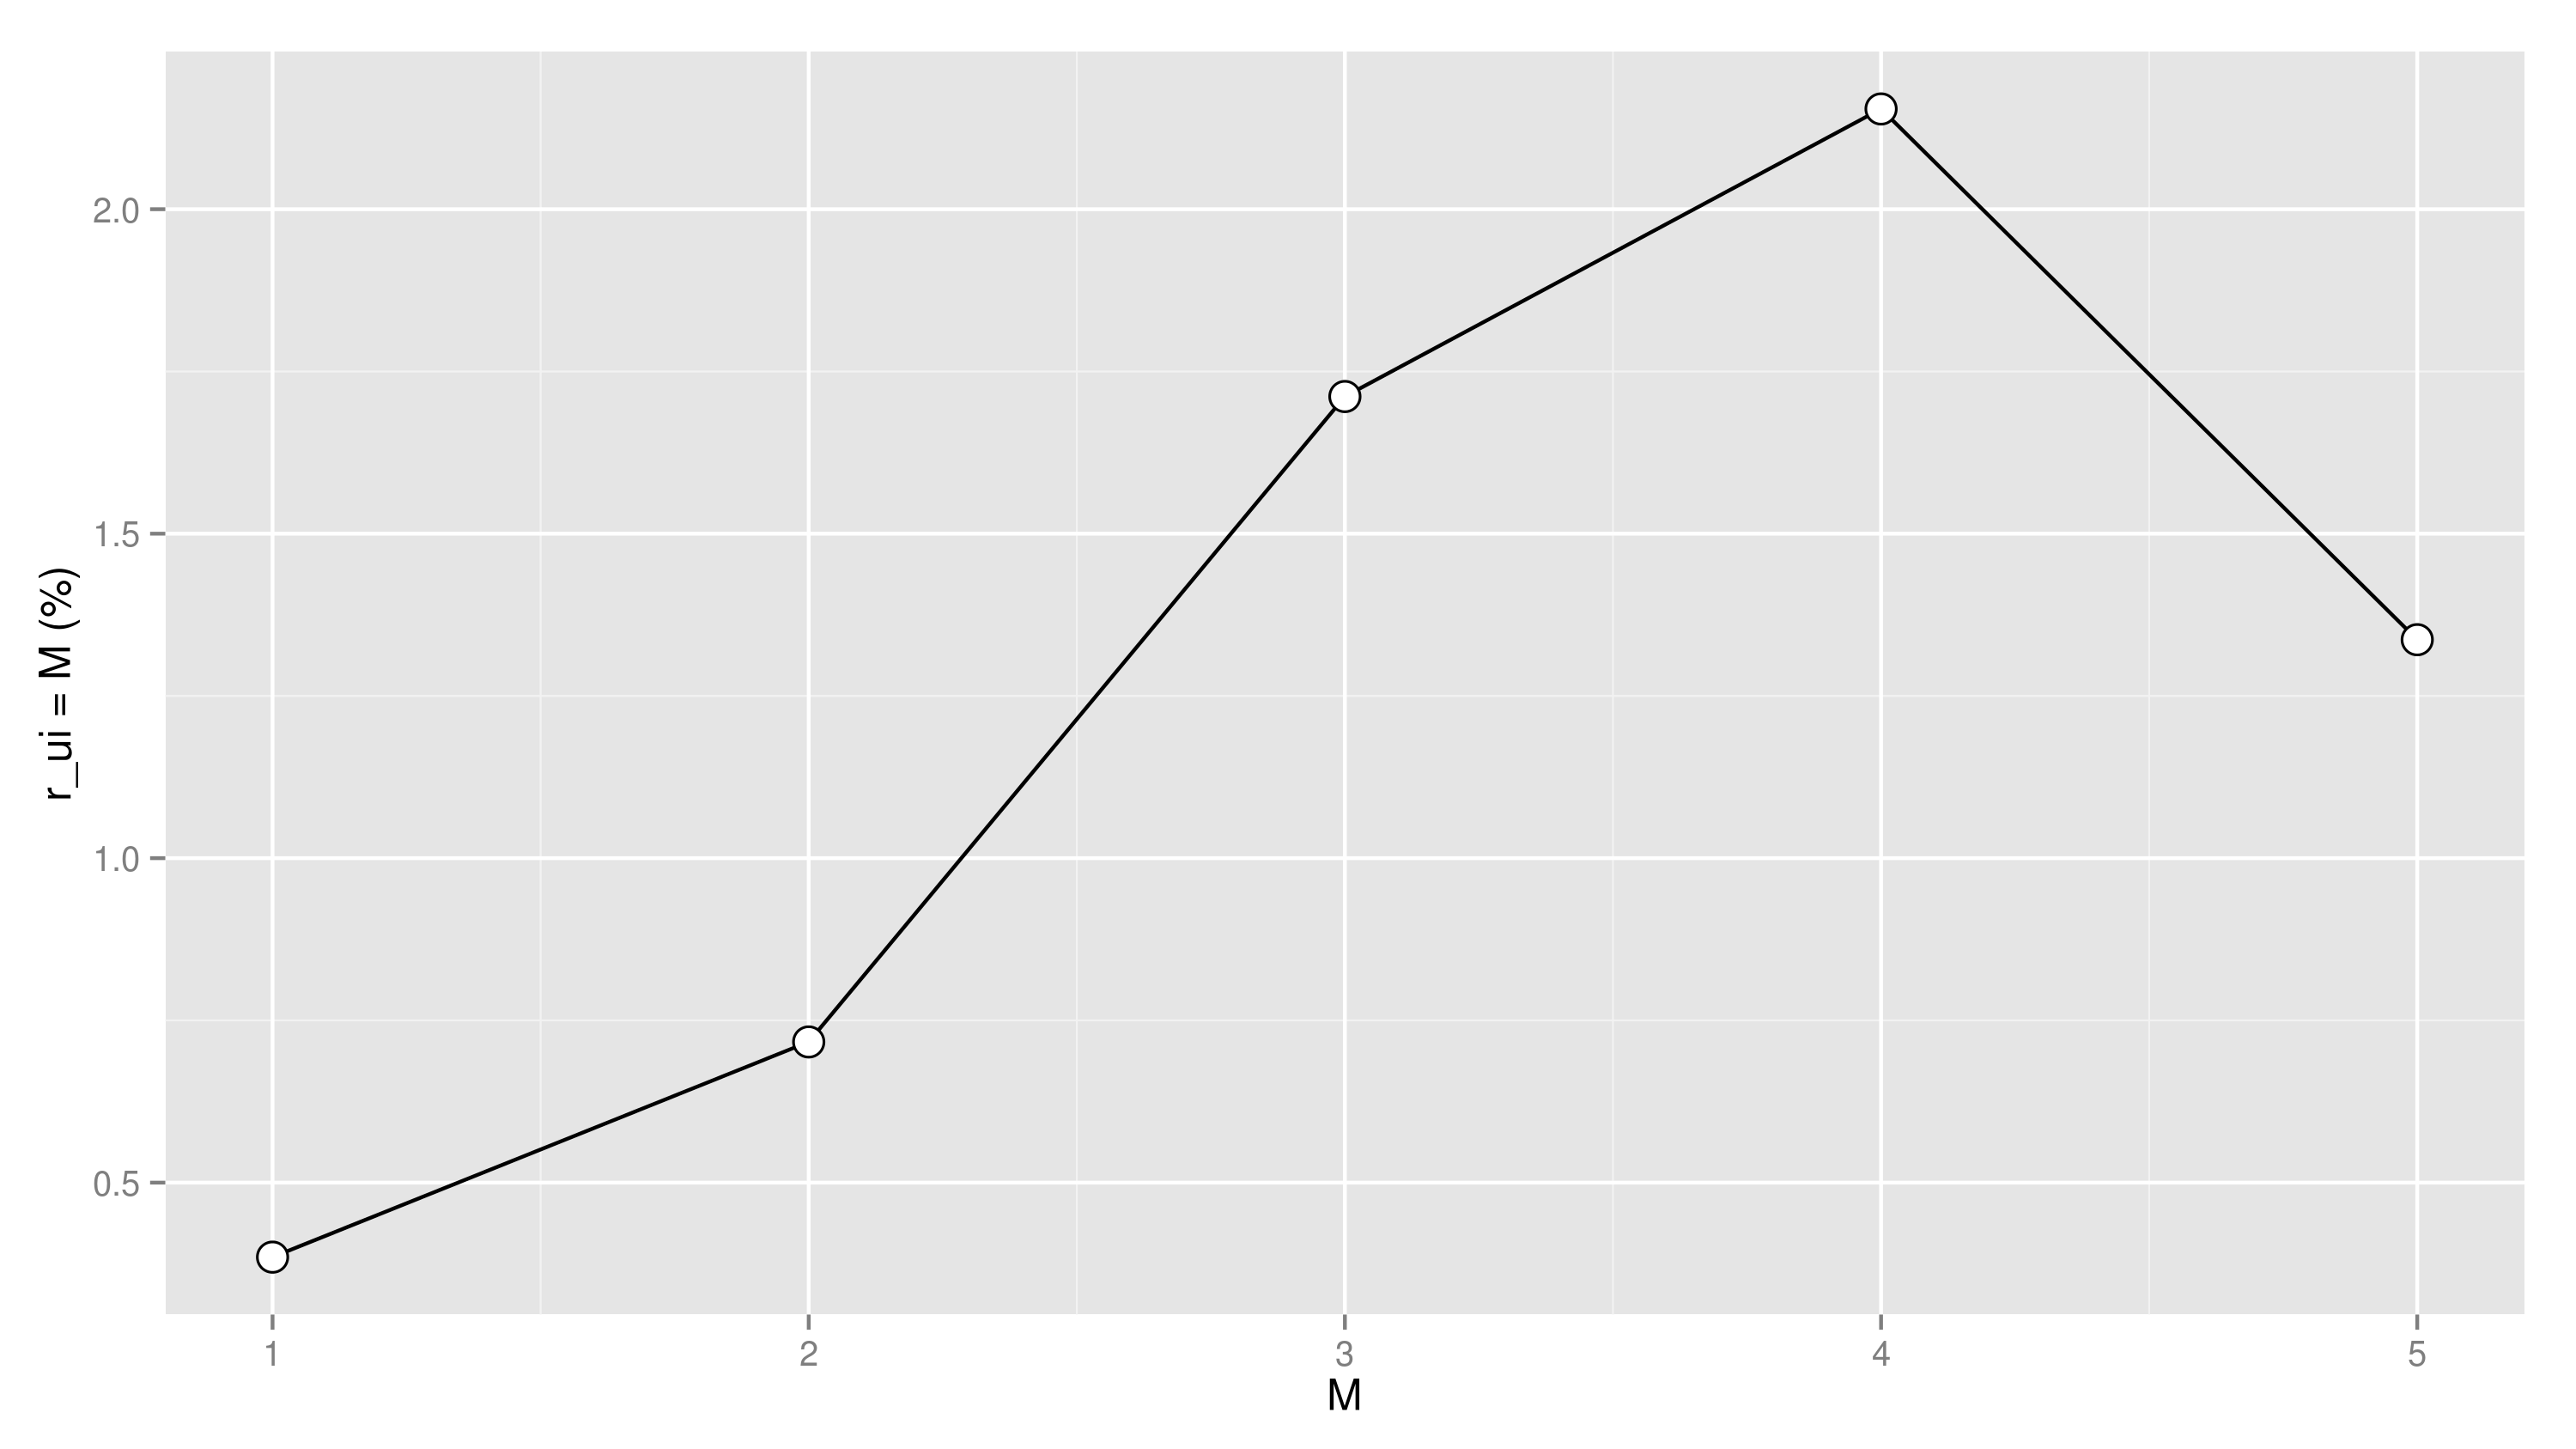
\includegraphics[width=1\textwidth]{img/percentual_M}
    \end{center}
    \caption{Percentual de avaliações por valor de $M$}
    \label{fig:percentual_M}
\end{figure}

\begin{figure}[htp]
    \begin{center}
    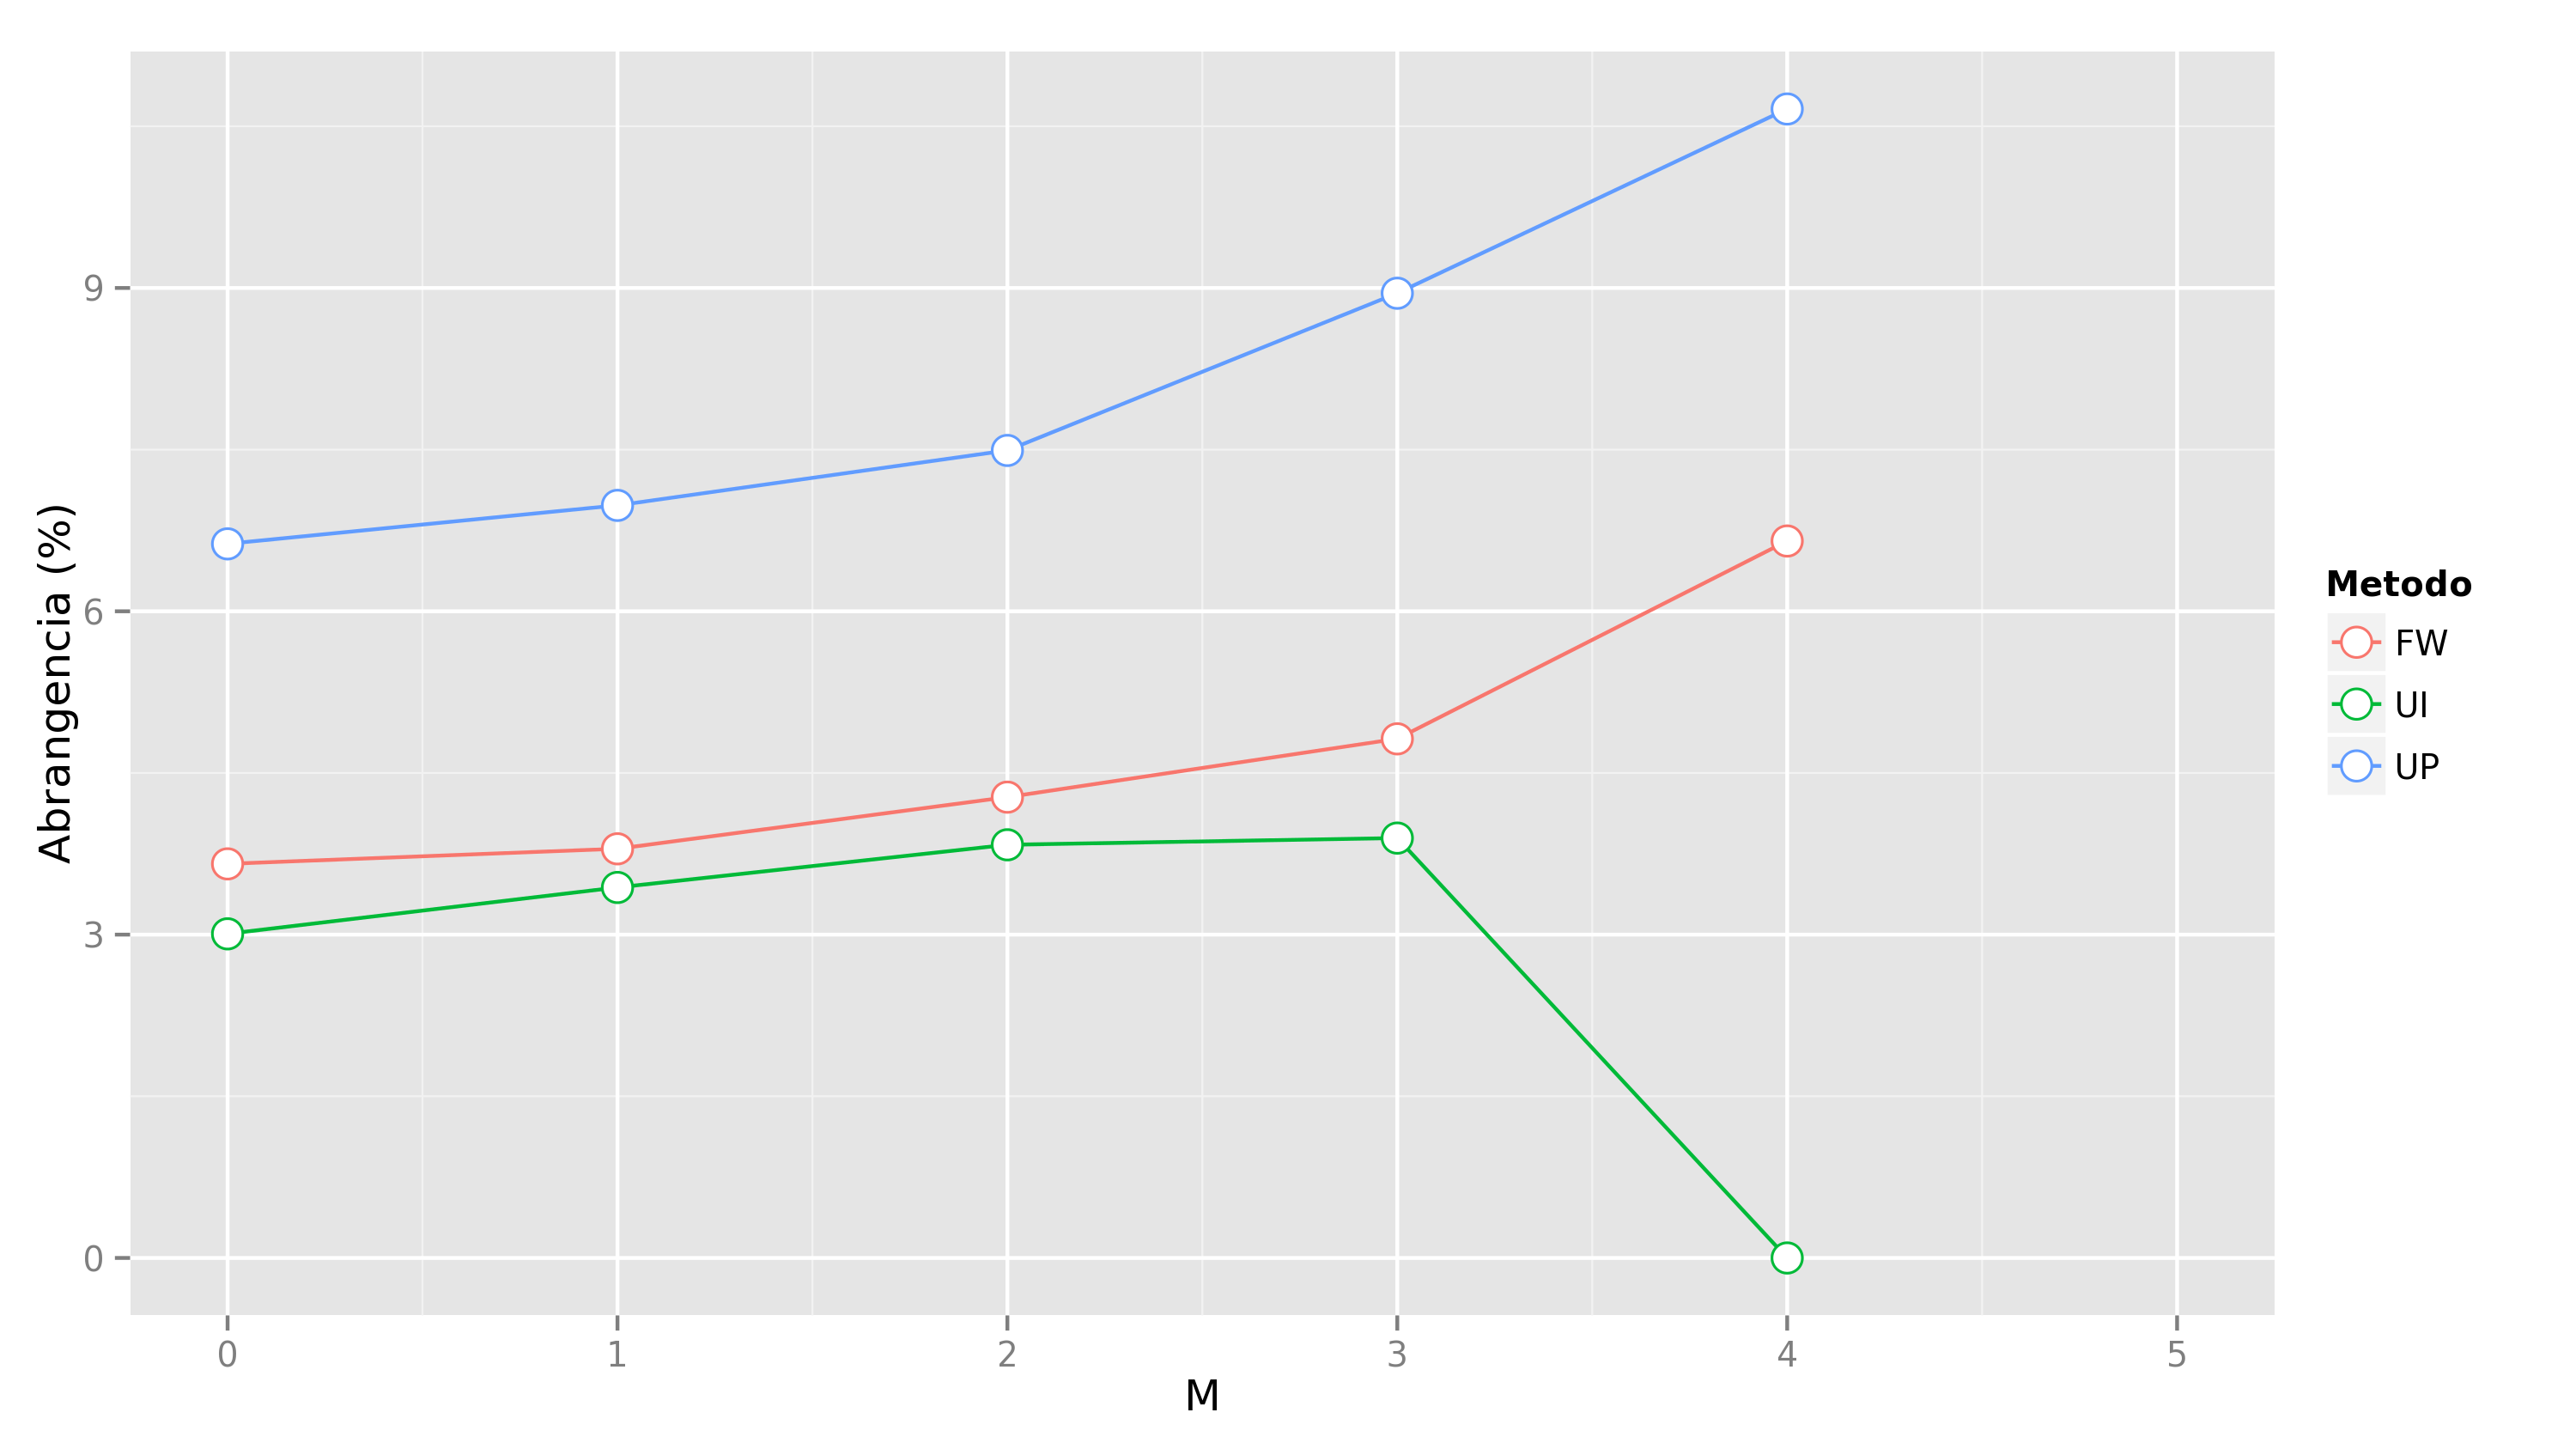
\includegraphics[width=1\textwidth]{img/recall_M}
    \end{center}
    \caption{Abrangência em função do valor mínimo para avaliações positivas $M$}
    \label{fig:recall_M}
\end{figure}

\begin{figure}[htp]
    \begin{center}
    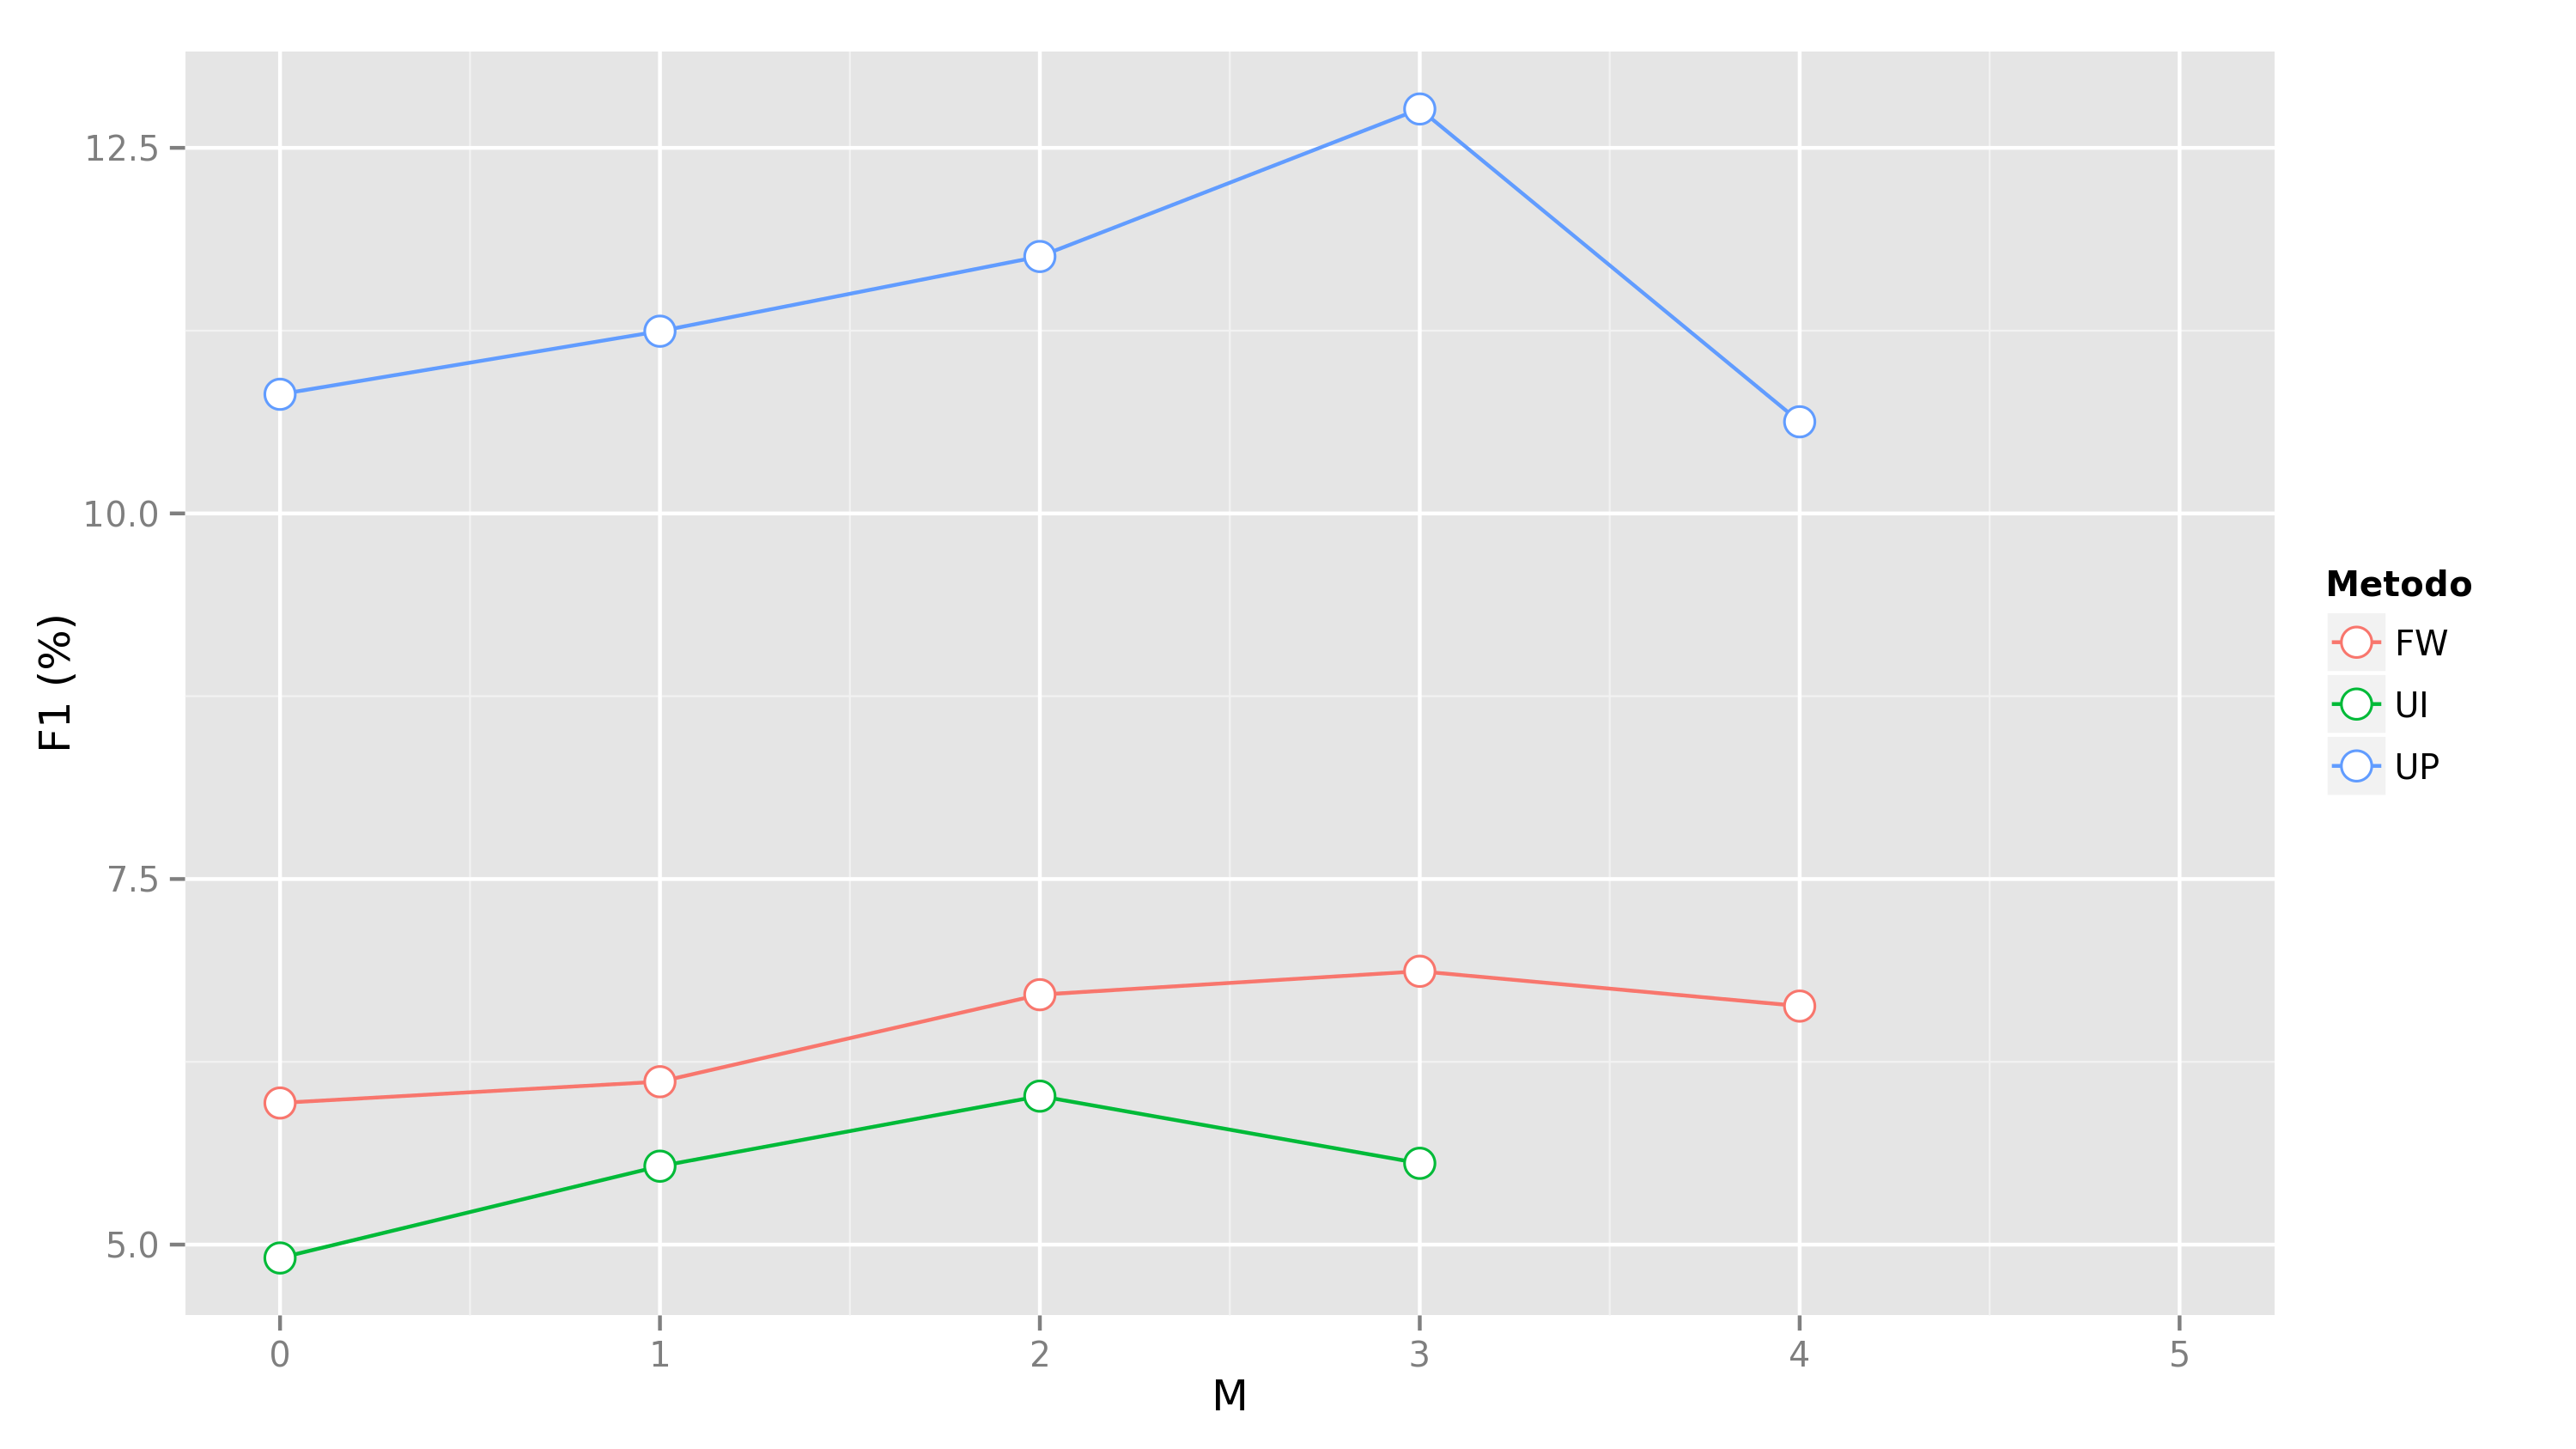
\includegraphics[width=1\textwidth]{img/F1_M}
    \end{center}
    \caption{Medida $F_1$ em função do valor mínimo para avaliações positivas $M$}
    \label{fig:F1_M}
\end{figure}

\begin{figure}[htp]
    \begin{center}
    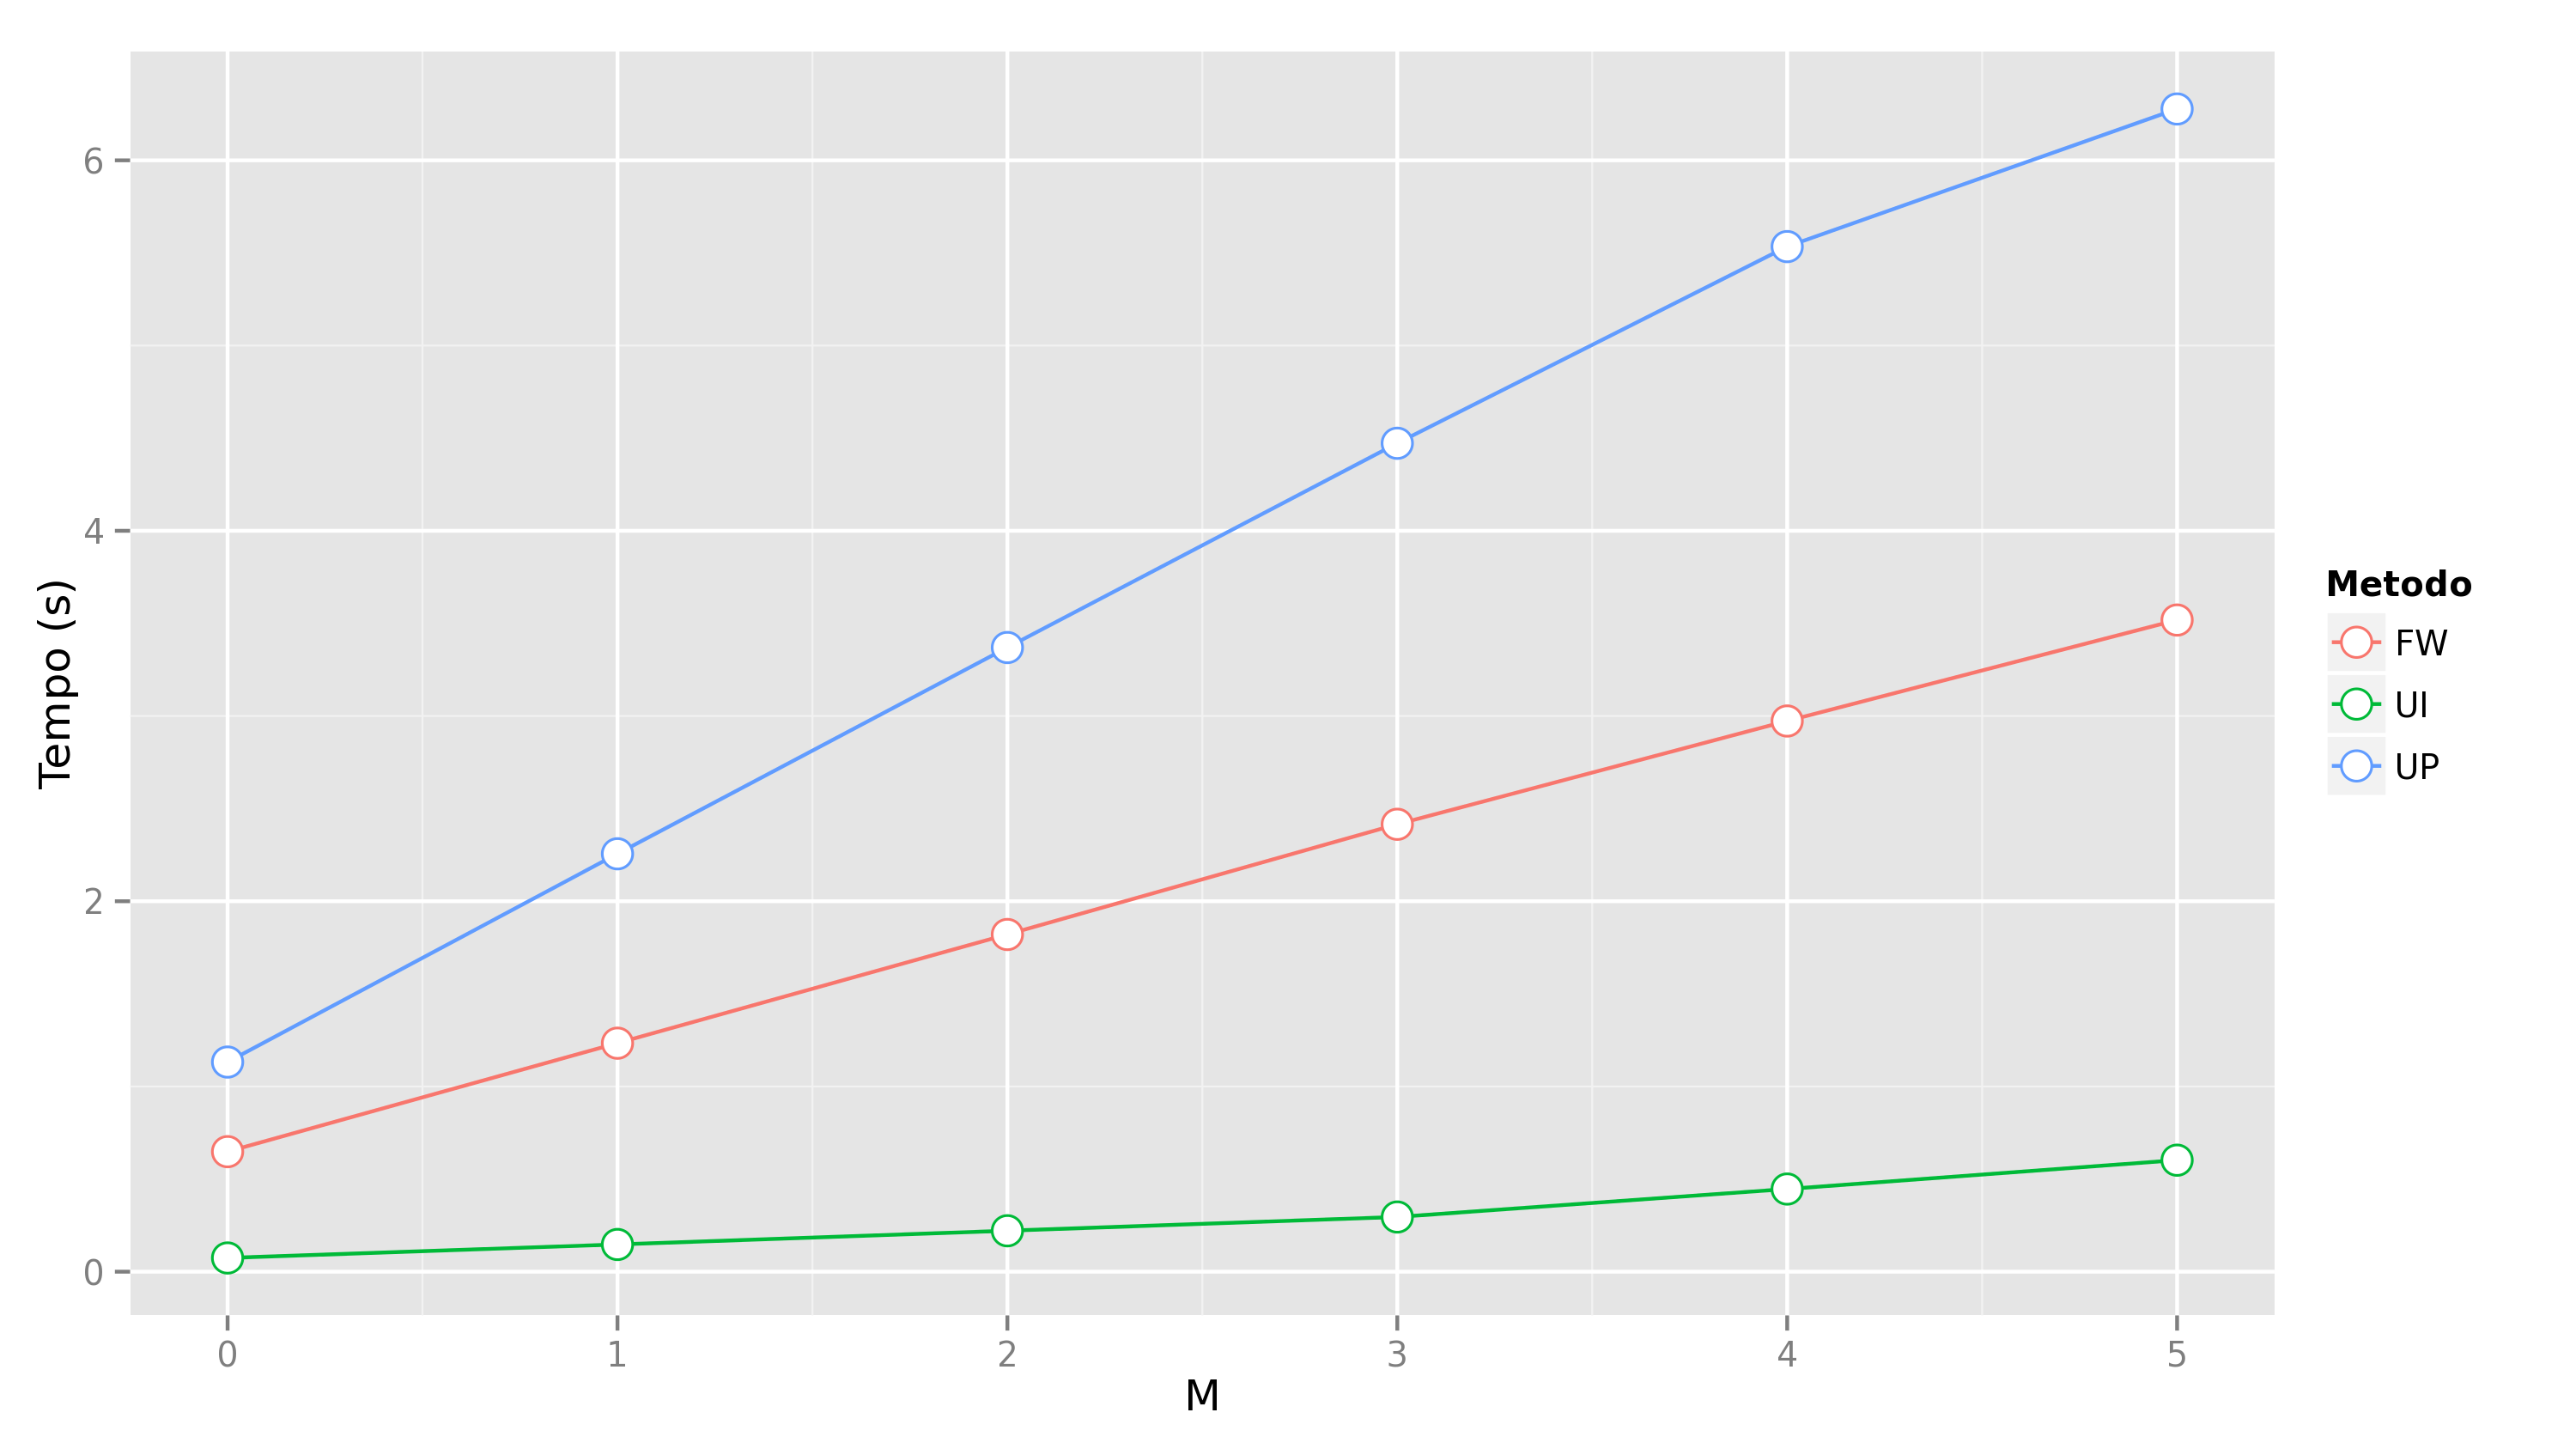
\includegraphics[width=1\textwidth]{img/time_M}
    \end{center}
    \caption{Tempo de execução em função do valor mínimo para avaliações positivas $M$}
    \label{fig:time_M}
\end{figure}

\section{Número de vizinhos mais próximos $k$} % (fold)
\label{sec:n_mero_de_vizinhos_mais_pr_ximos_}

O único método que recomenda itens com base nos vizinhos mais próximos é o UP. Percebe-se que com o aumento de $k$, a precisão e a abrangência caem, pois a vizinhança se torna excessivamente grande e repleta de usuários sem muita similaridade com o usuário-teste. Pode-se observar que o valor máximo de precisão e acurácia ocorre para $k=20$ (Figura \ref{fig:F1_k}).

\begin{figure}[htp]
    \begin{center}
    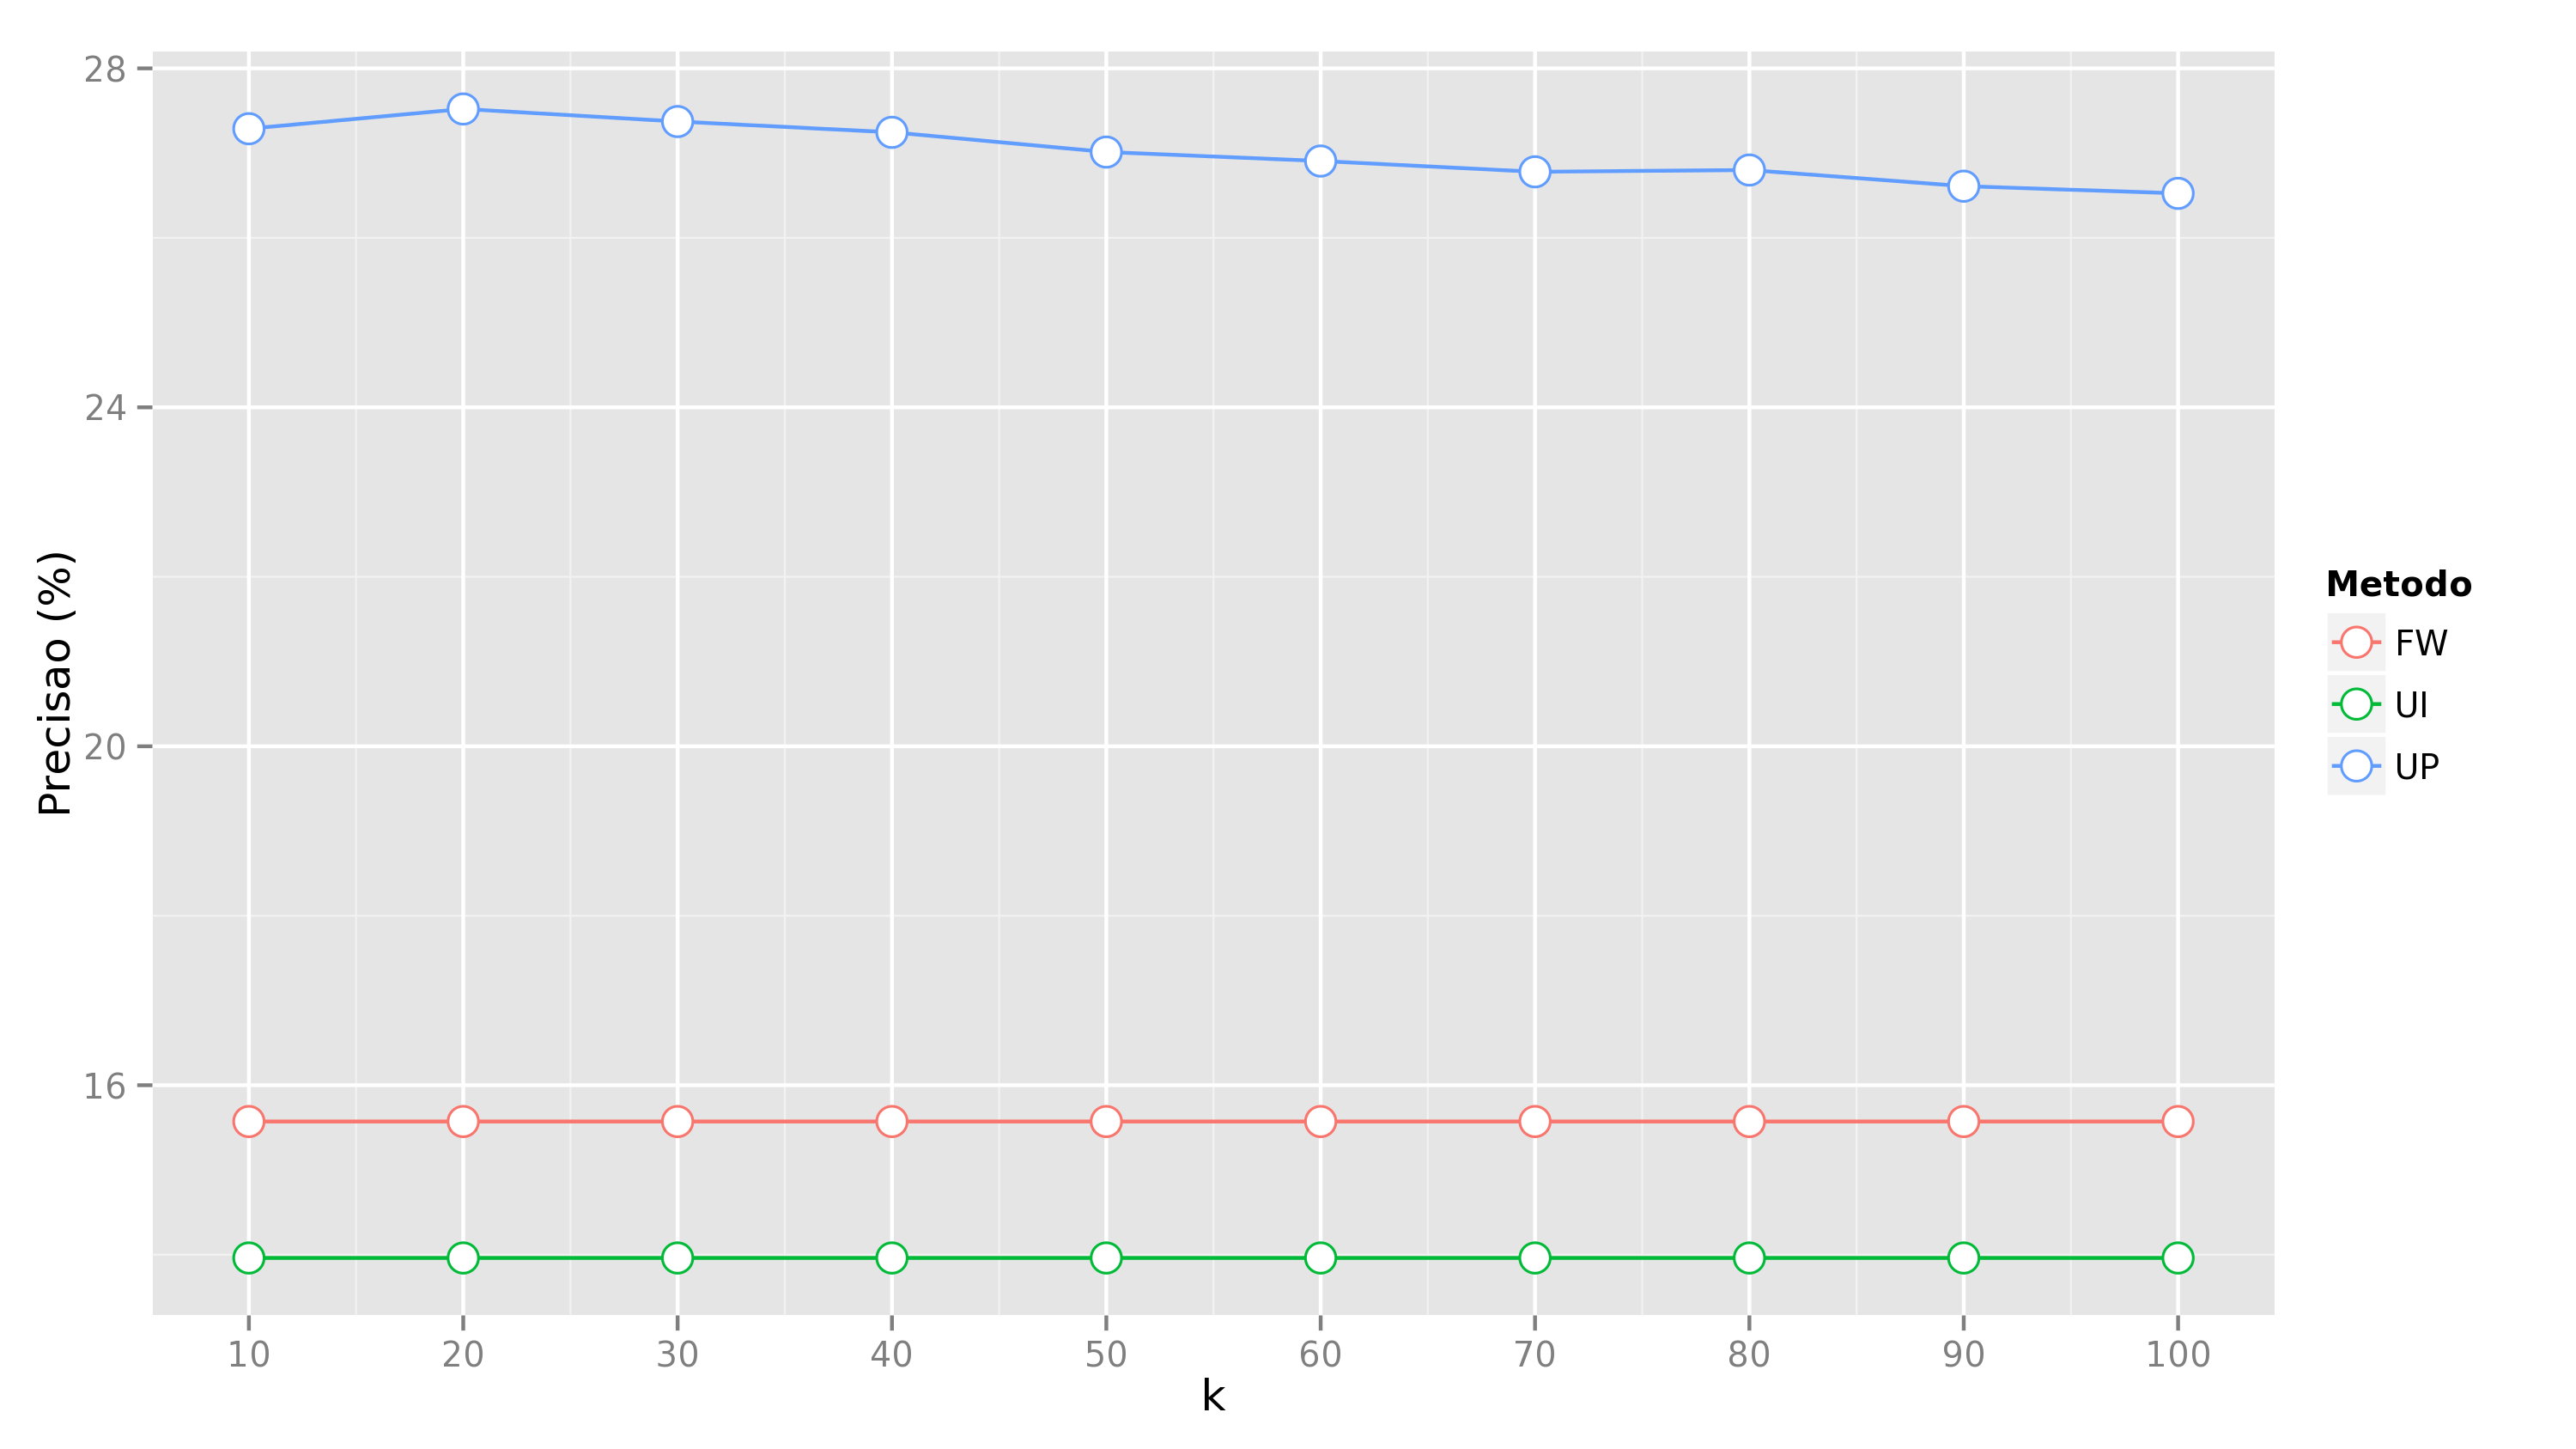
\includegraphics[width=1\textwidth]{img/precision_k}
    \end{center}
    \caption{Precisão em função do número de vizinhos mais próximos $k$}
    \label{fig:precision_k}
\end{figure}


\begin{figure}[htp]
    \begin{center}
    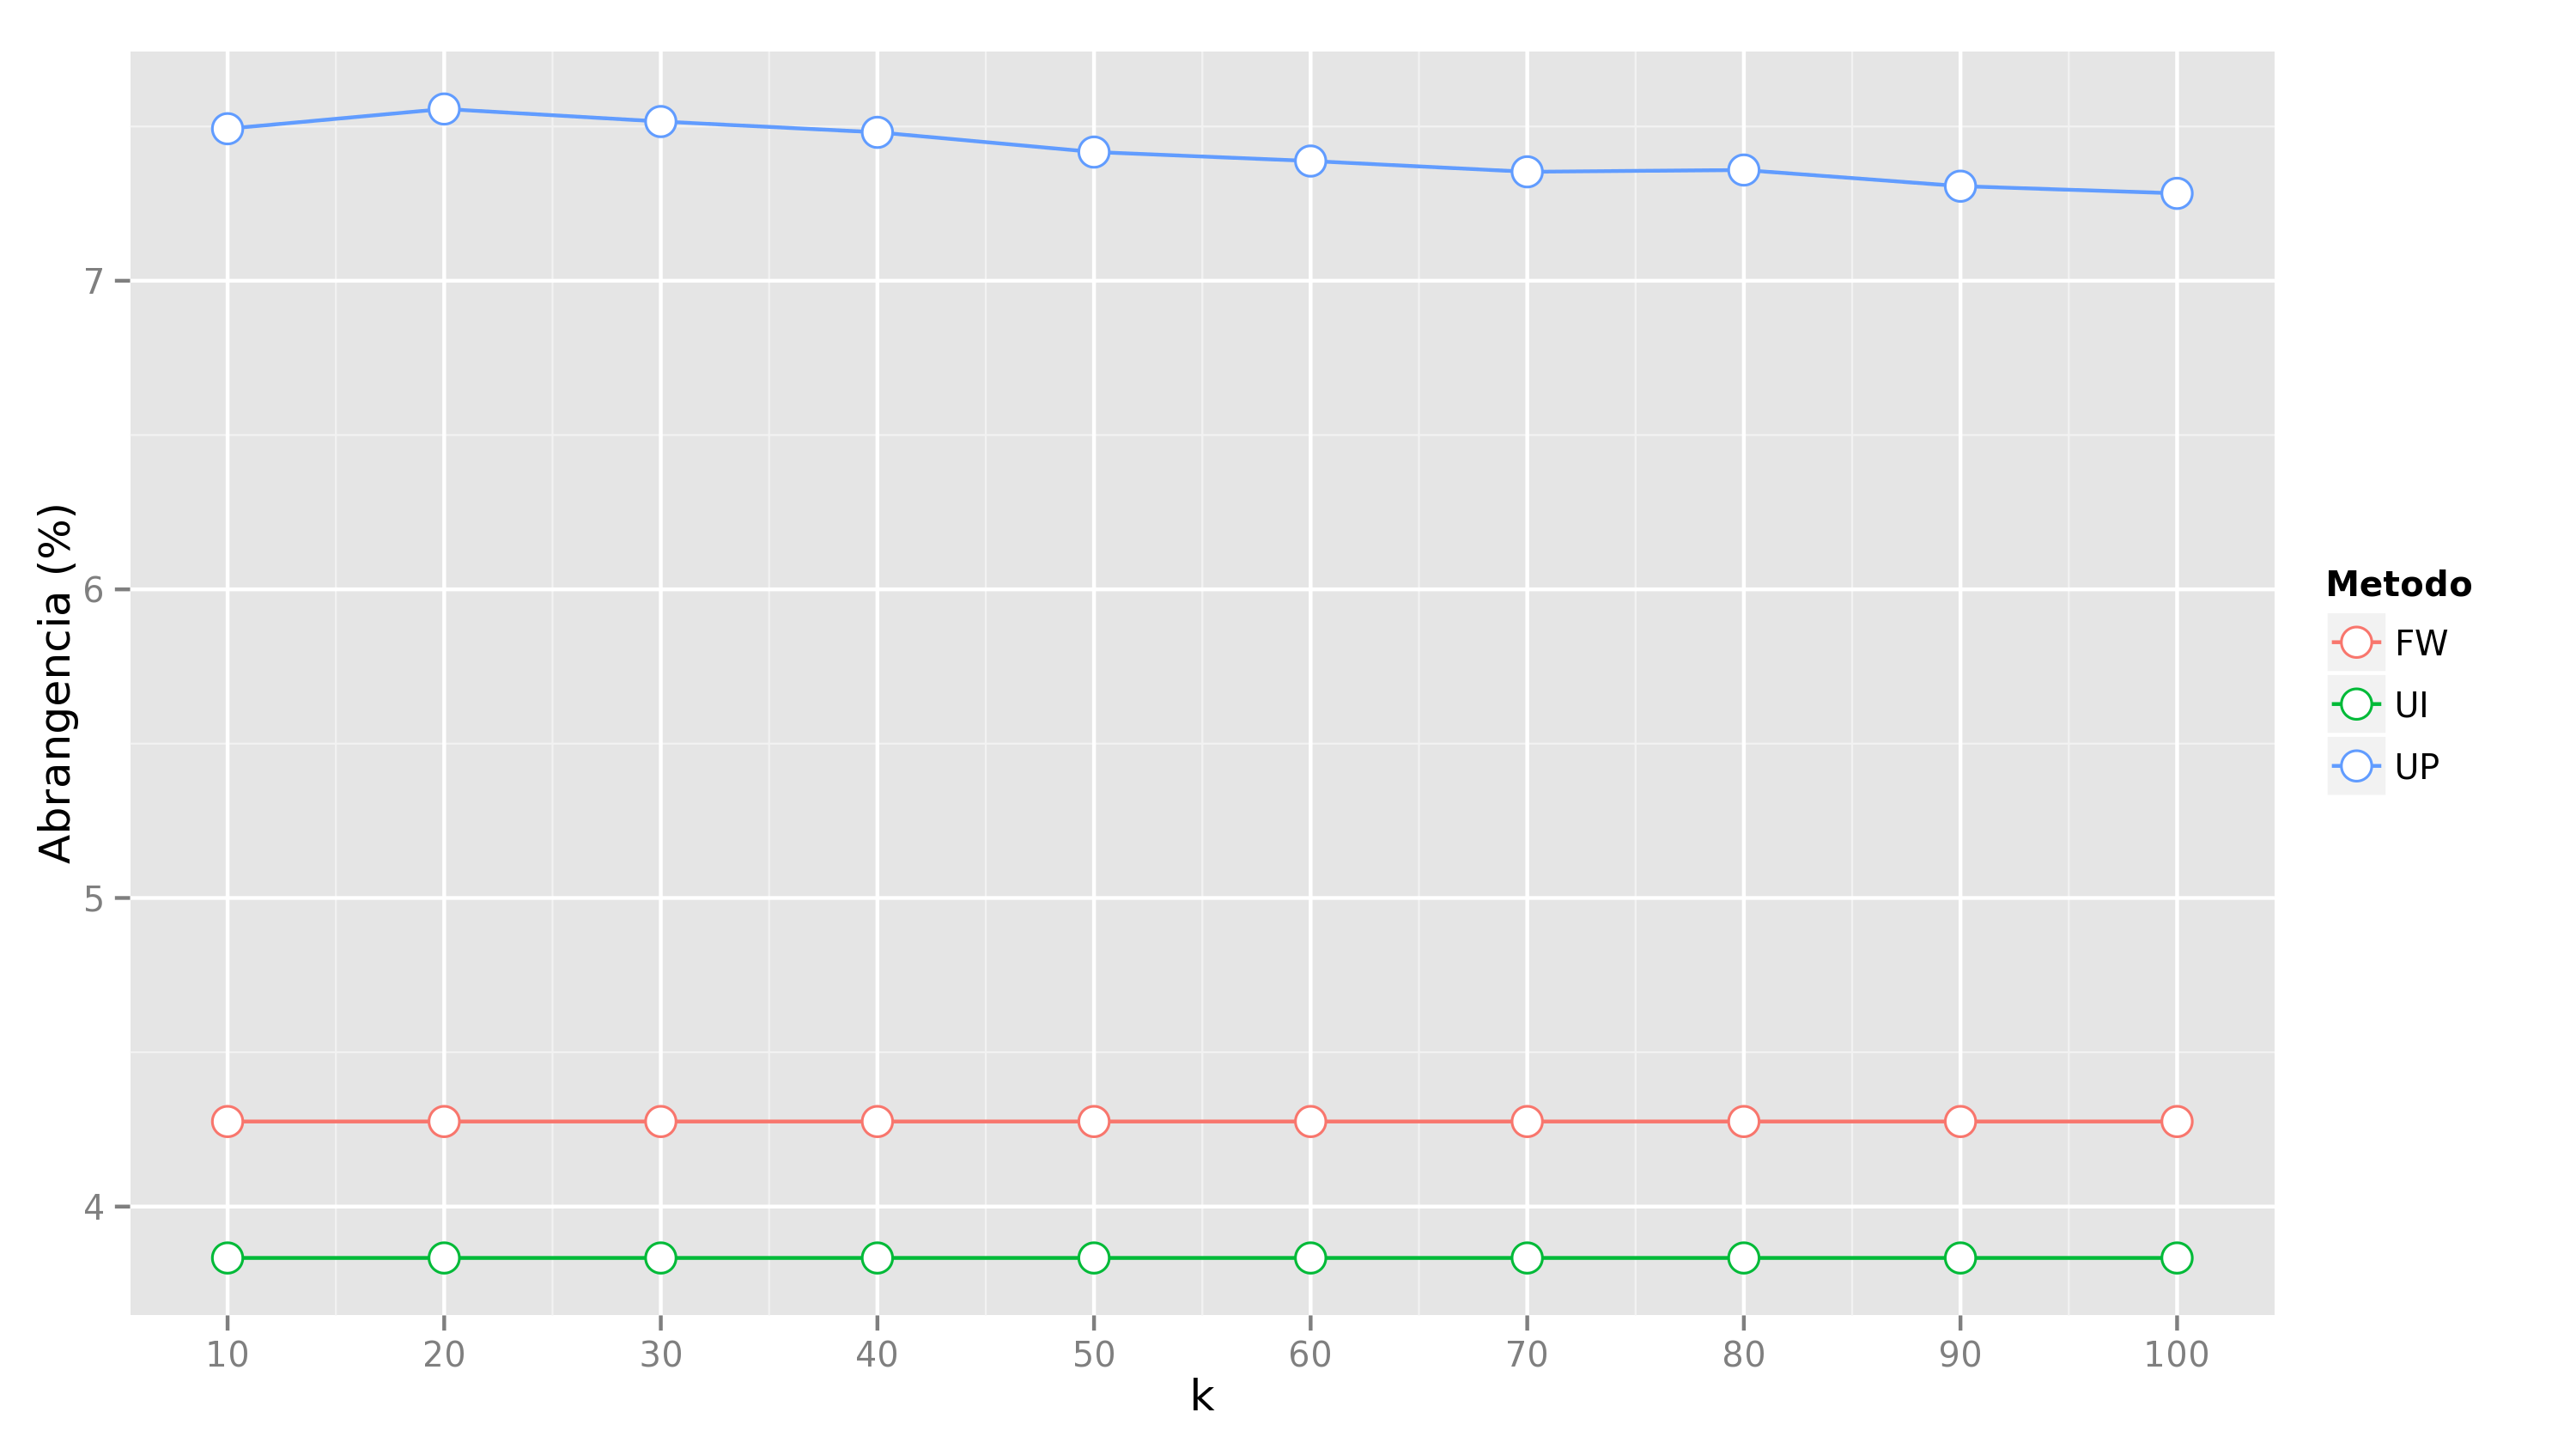
\includegraphics[width=1\textwidth]{img/recall_k}
    \end{center}
    \caption{Abrangência em função do número de vizinhos mais próximos $k$}
    \label{fig:recall_k}
\end{figure}

\begin{figure}[htp]
    \begin{center}
    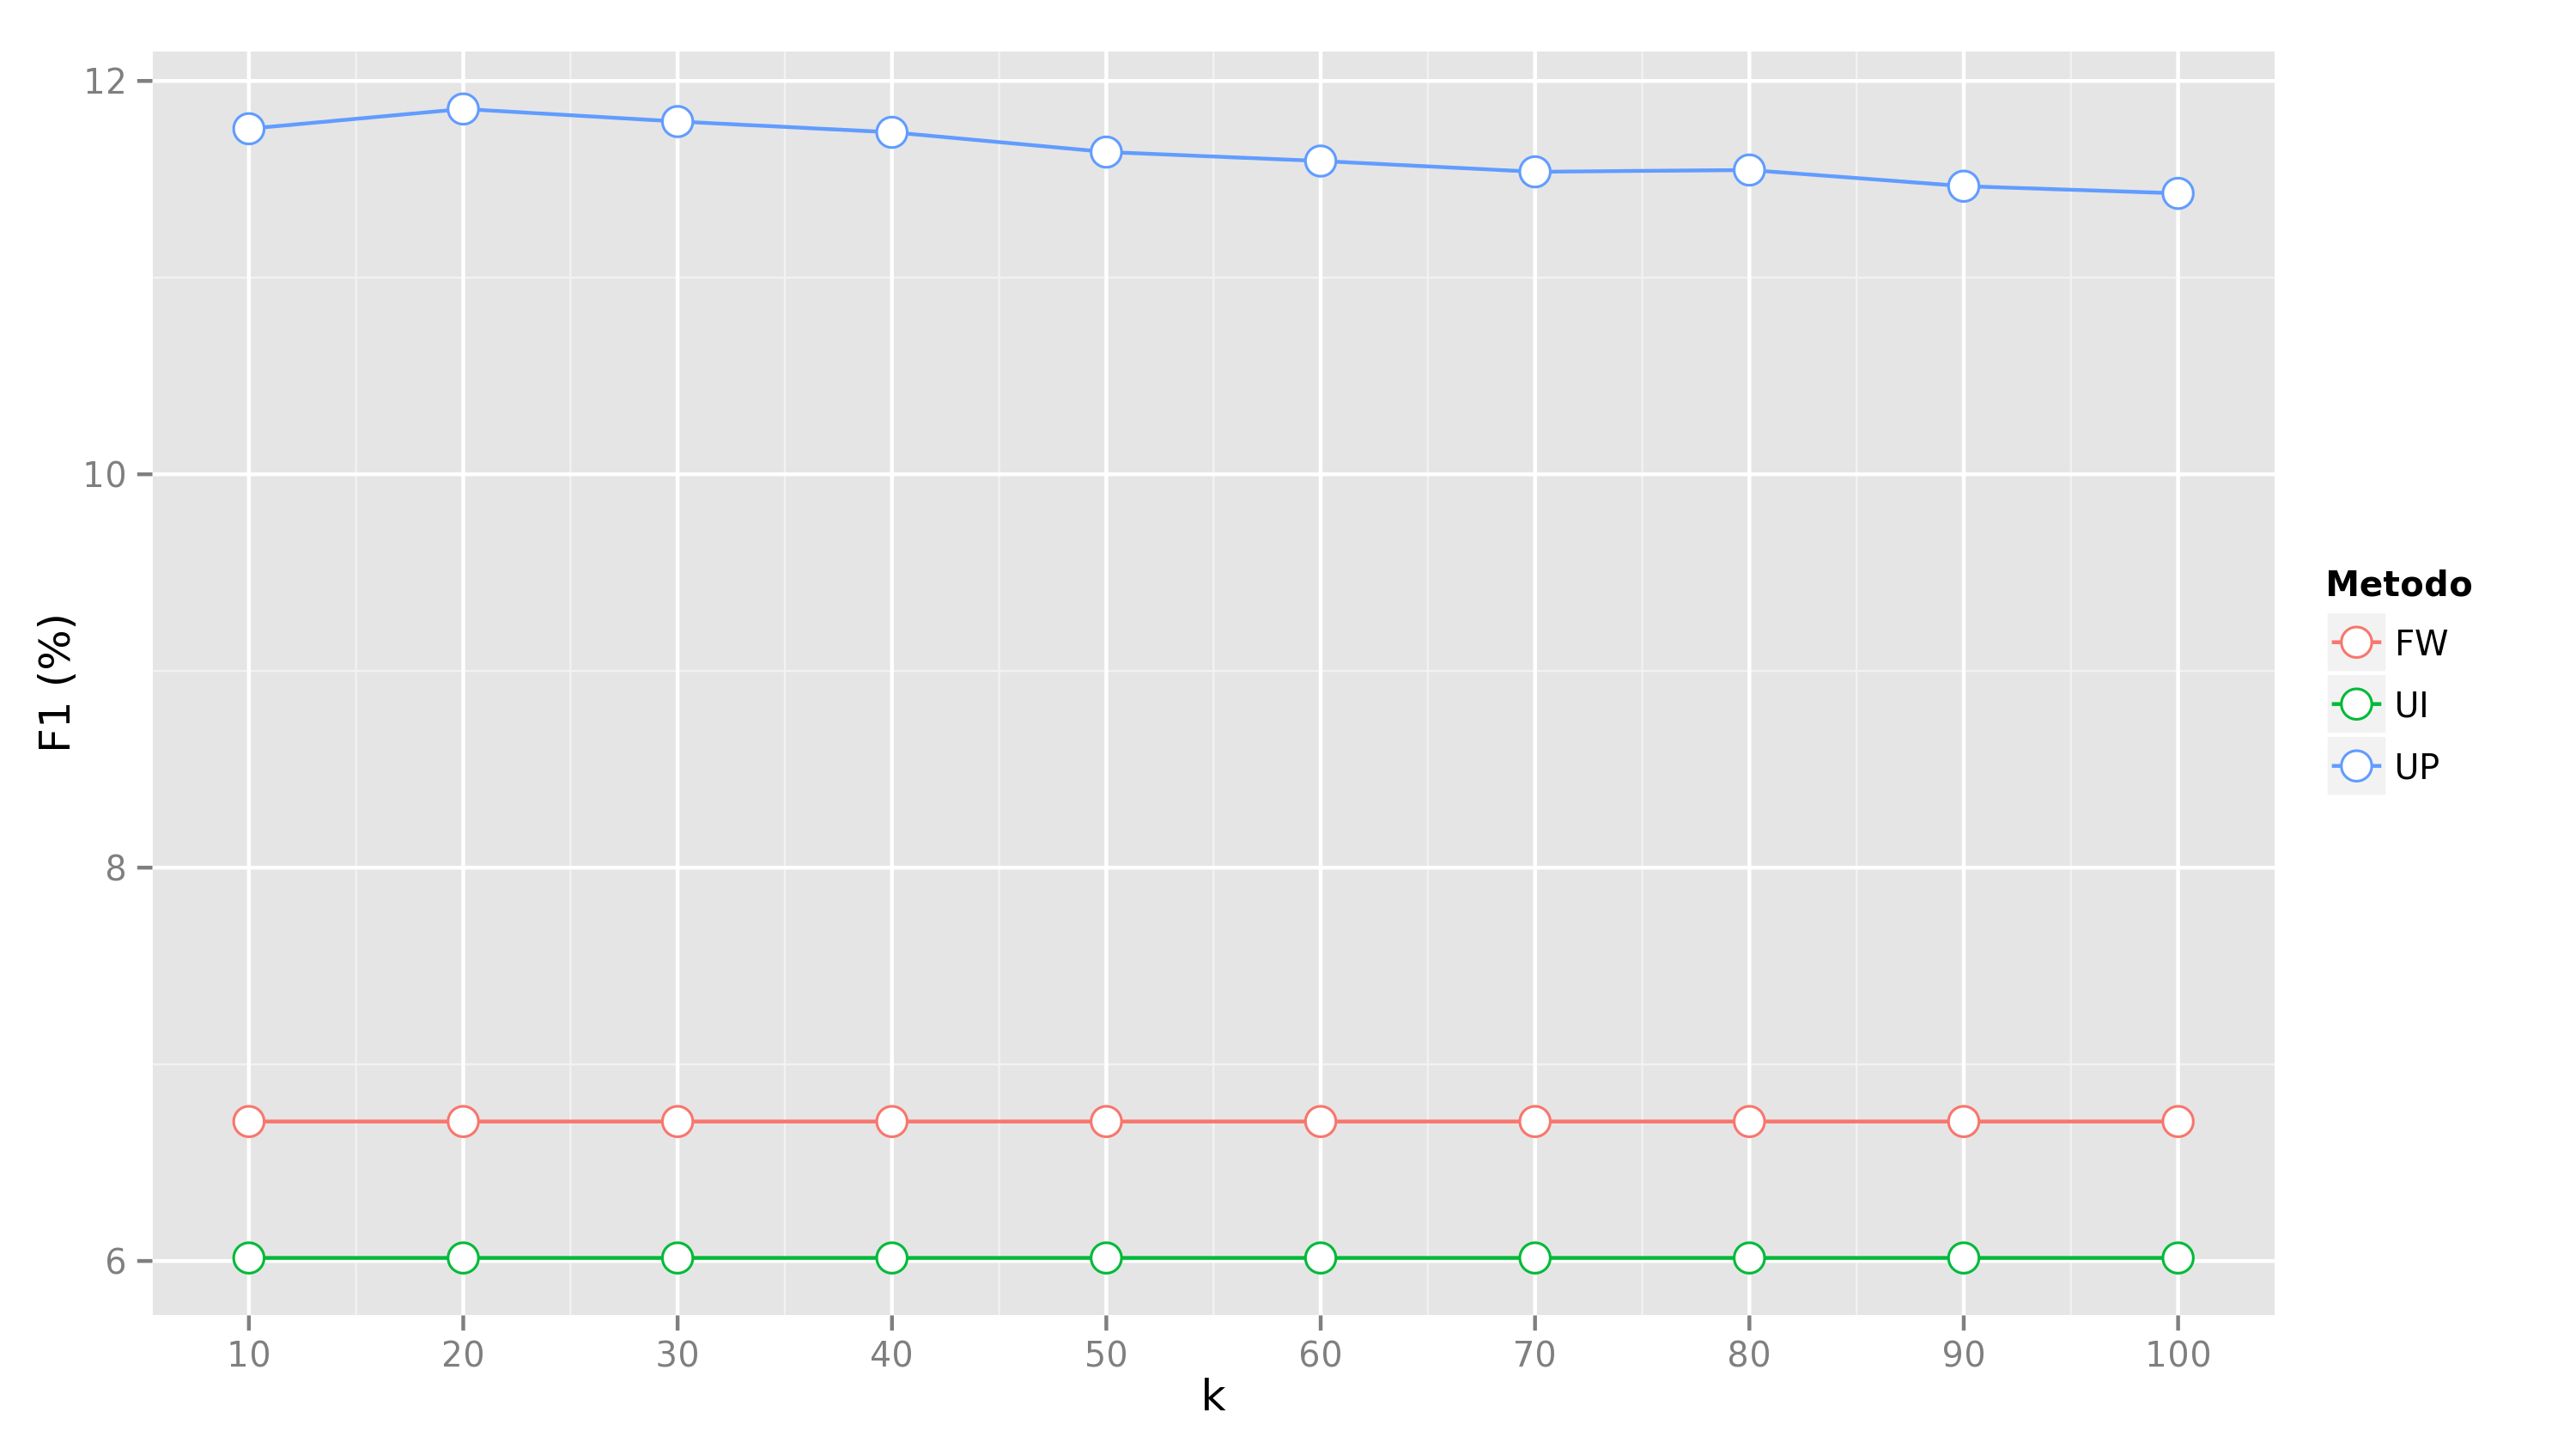
\includegraphics[width=1\textwidth]{img/F1_k}
    \end{center}
    \caption{Medida $F_1$ em função do número de vizinhos mais próximos $k$}
    \label{fig:F1_k}
\end{figure}

%\begin{figure}[htp]
    %\begin{center}
   % 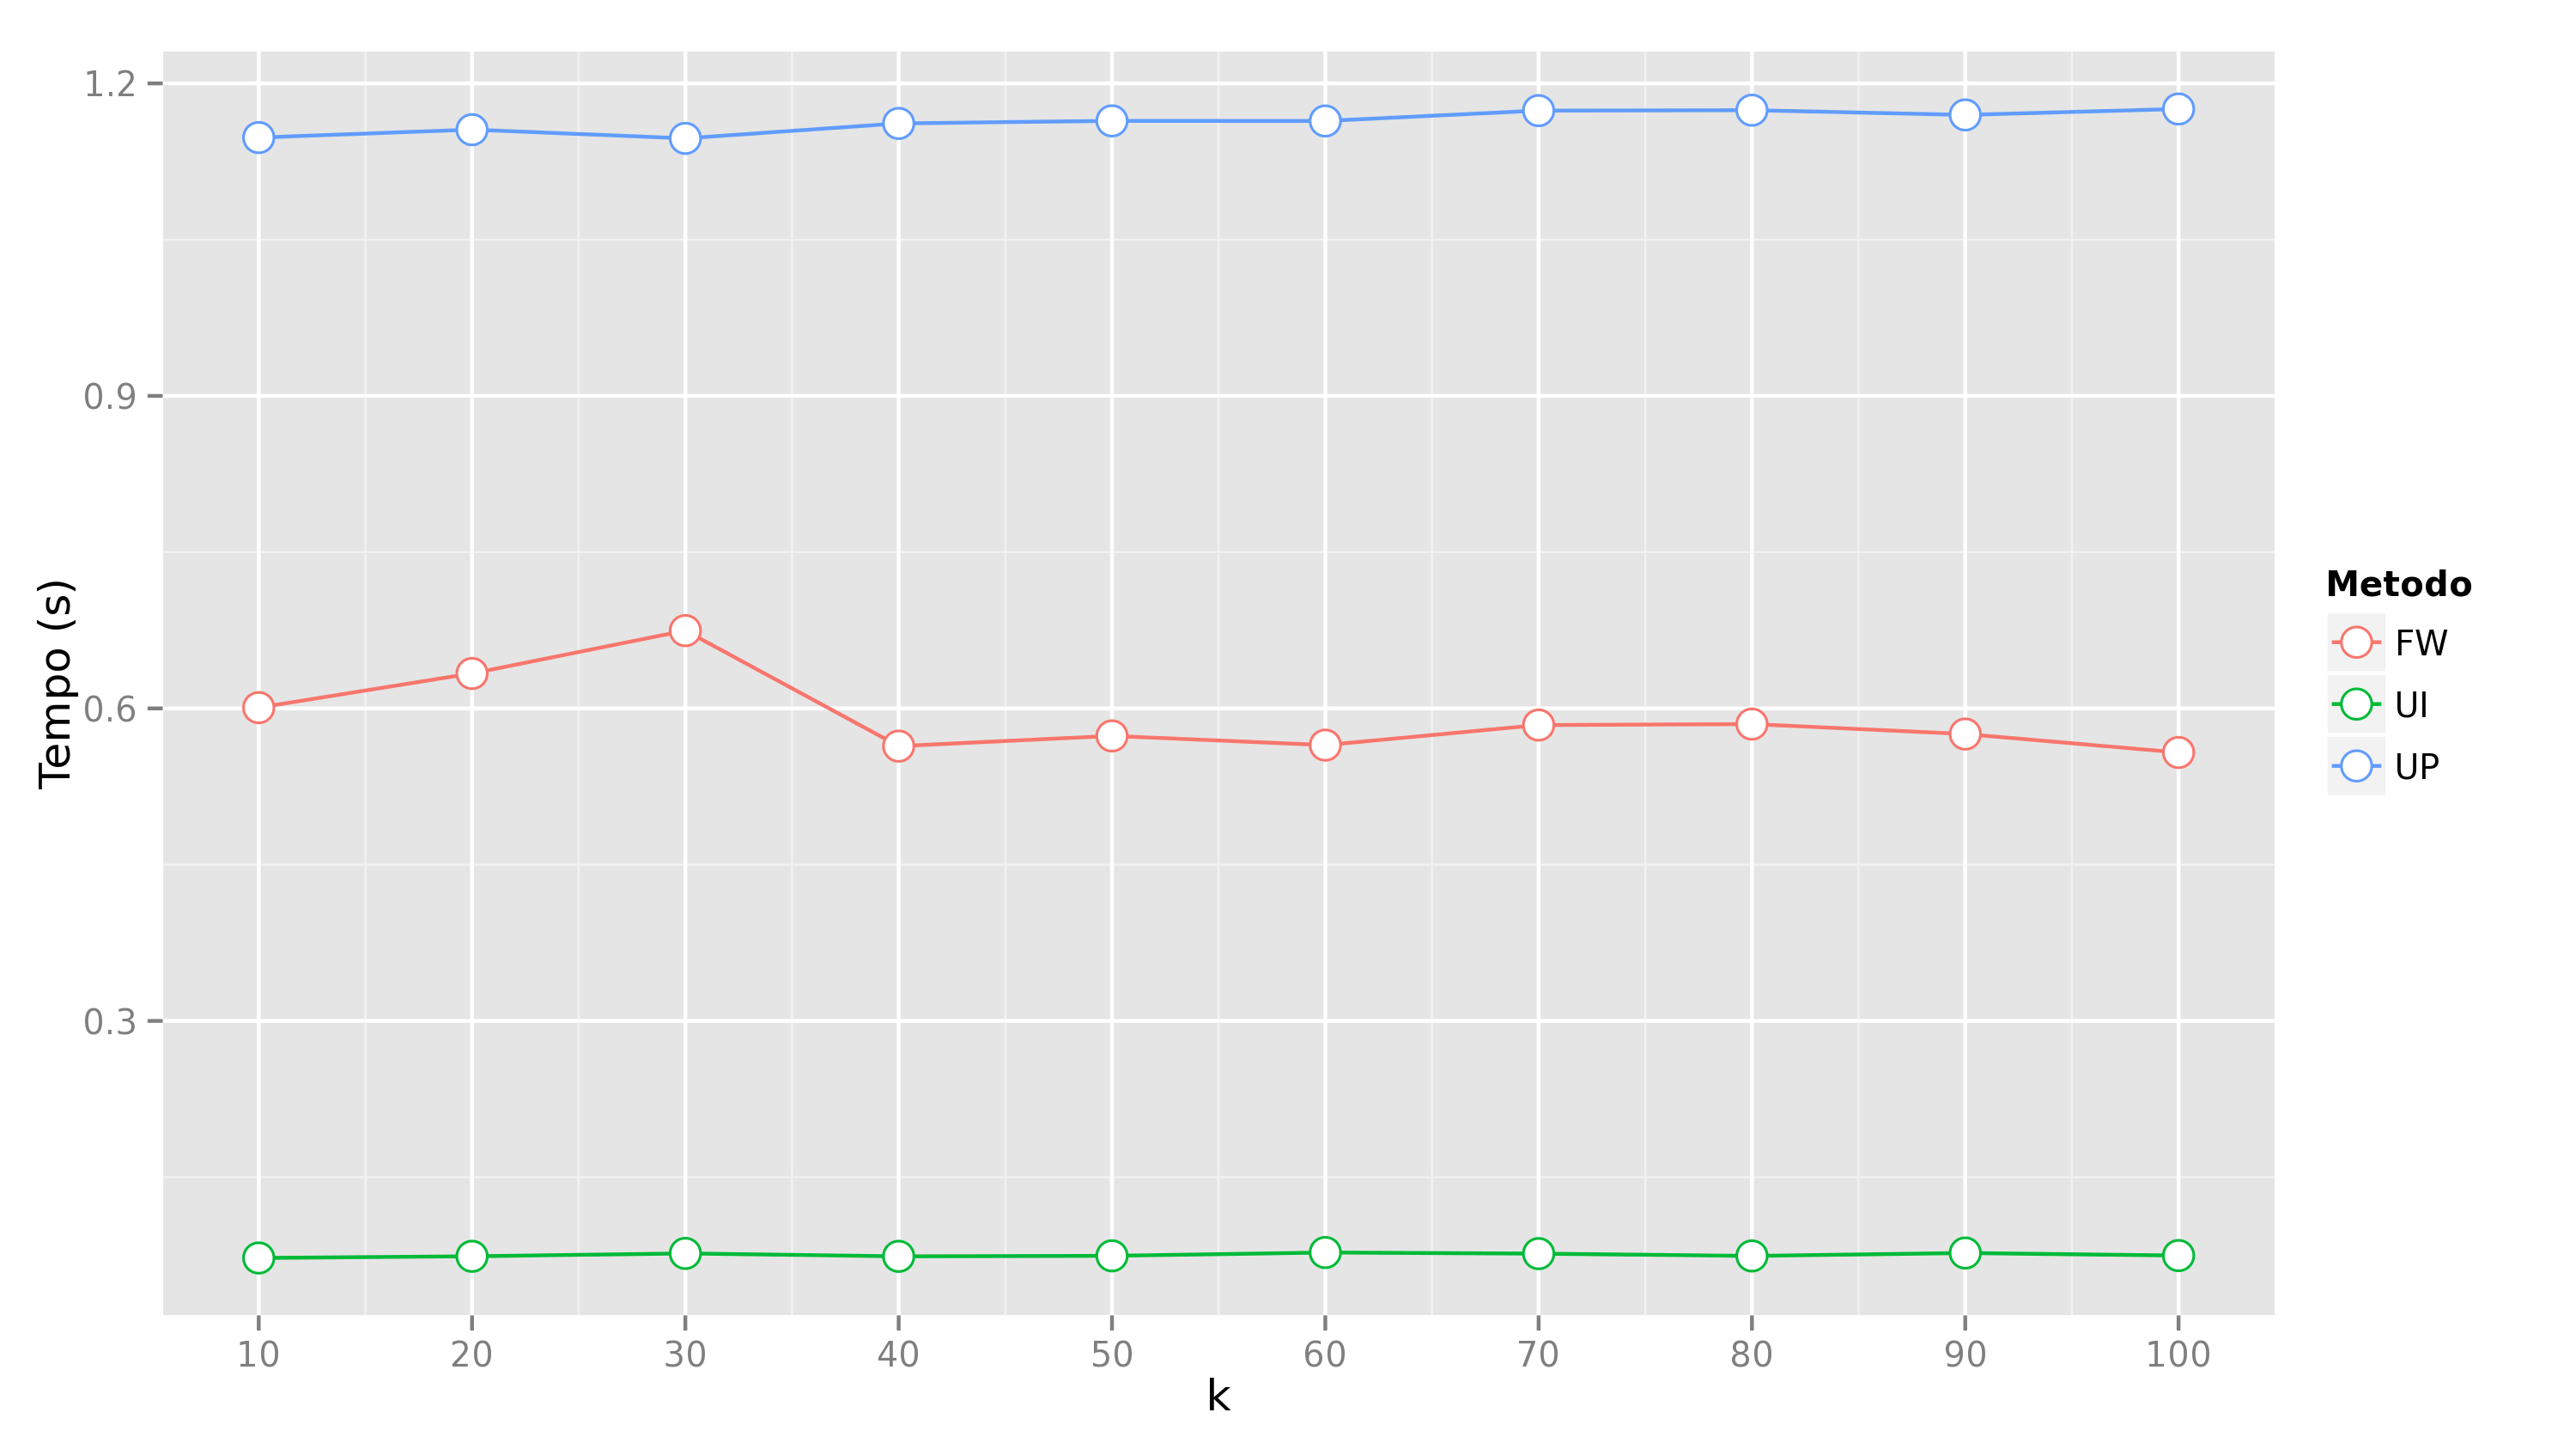
\includegraphics[width=1\textwidth]{img/time_k}
  %  \end{center}
 %   \label{fig:time_k}
%    \caption{Tempo de execução em função do número de vizinhos mais próximos $k$}
%\end{figure}

\section{Conjunto de atributos dos itens
 $\mathcal{F}$} % (fold)
\label{sec:conjunto_de_atributos_dos_itens_}

Para o banco de dados 100k-IMDB, o conjunto de atributos dos itens é $\mathcal{F}=$\{{data de lançamento, gênero, duração, orçamento, avaliação, votos\}. 


\begin{figure}[htp]
    \begin{center}
    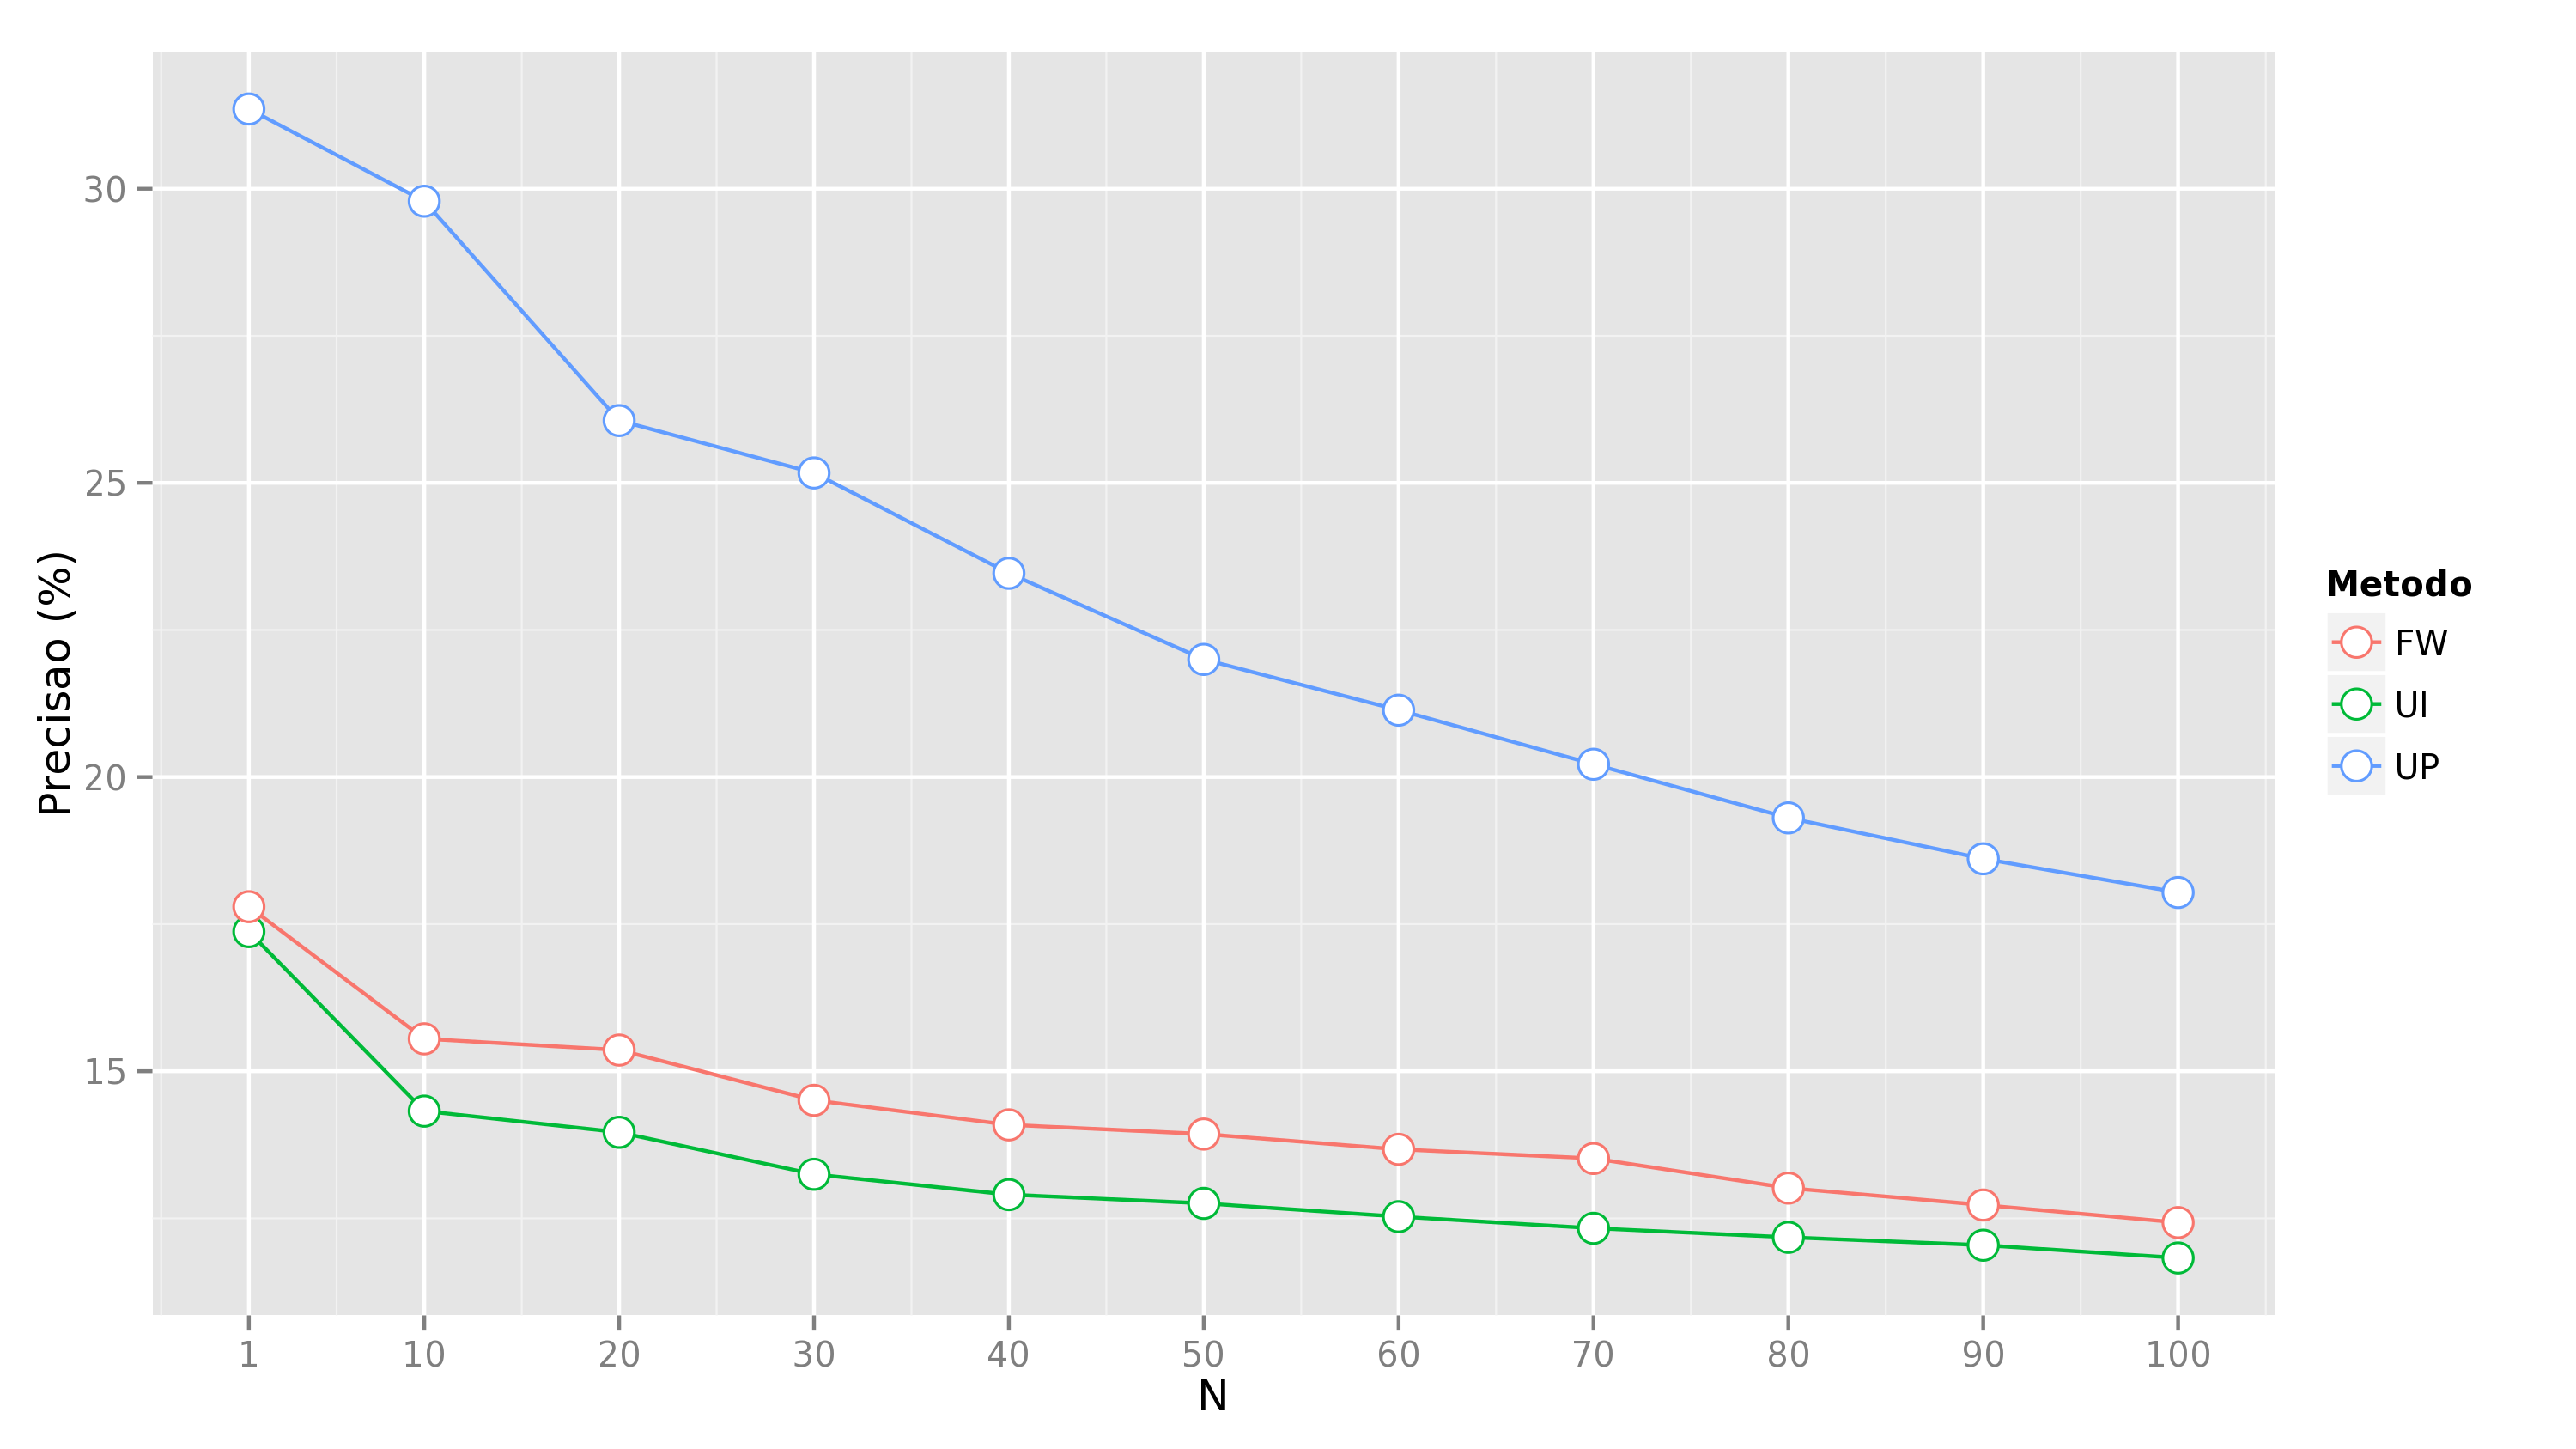
\includegraphics[width=1\textwidth]{img/precision_N_F}
    \end{center}
    \caption{Precisão em função do tamanho da lista de recomendações $N$}
    \label{fig:precision_N_F}
\end{figure}


\begin{figure}[htp]
    \begin{center}
    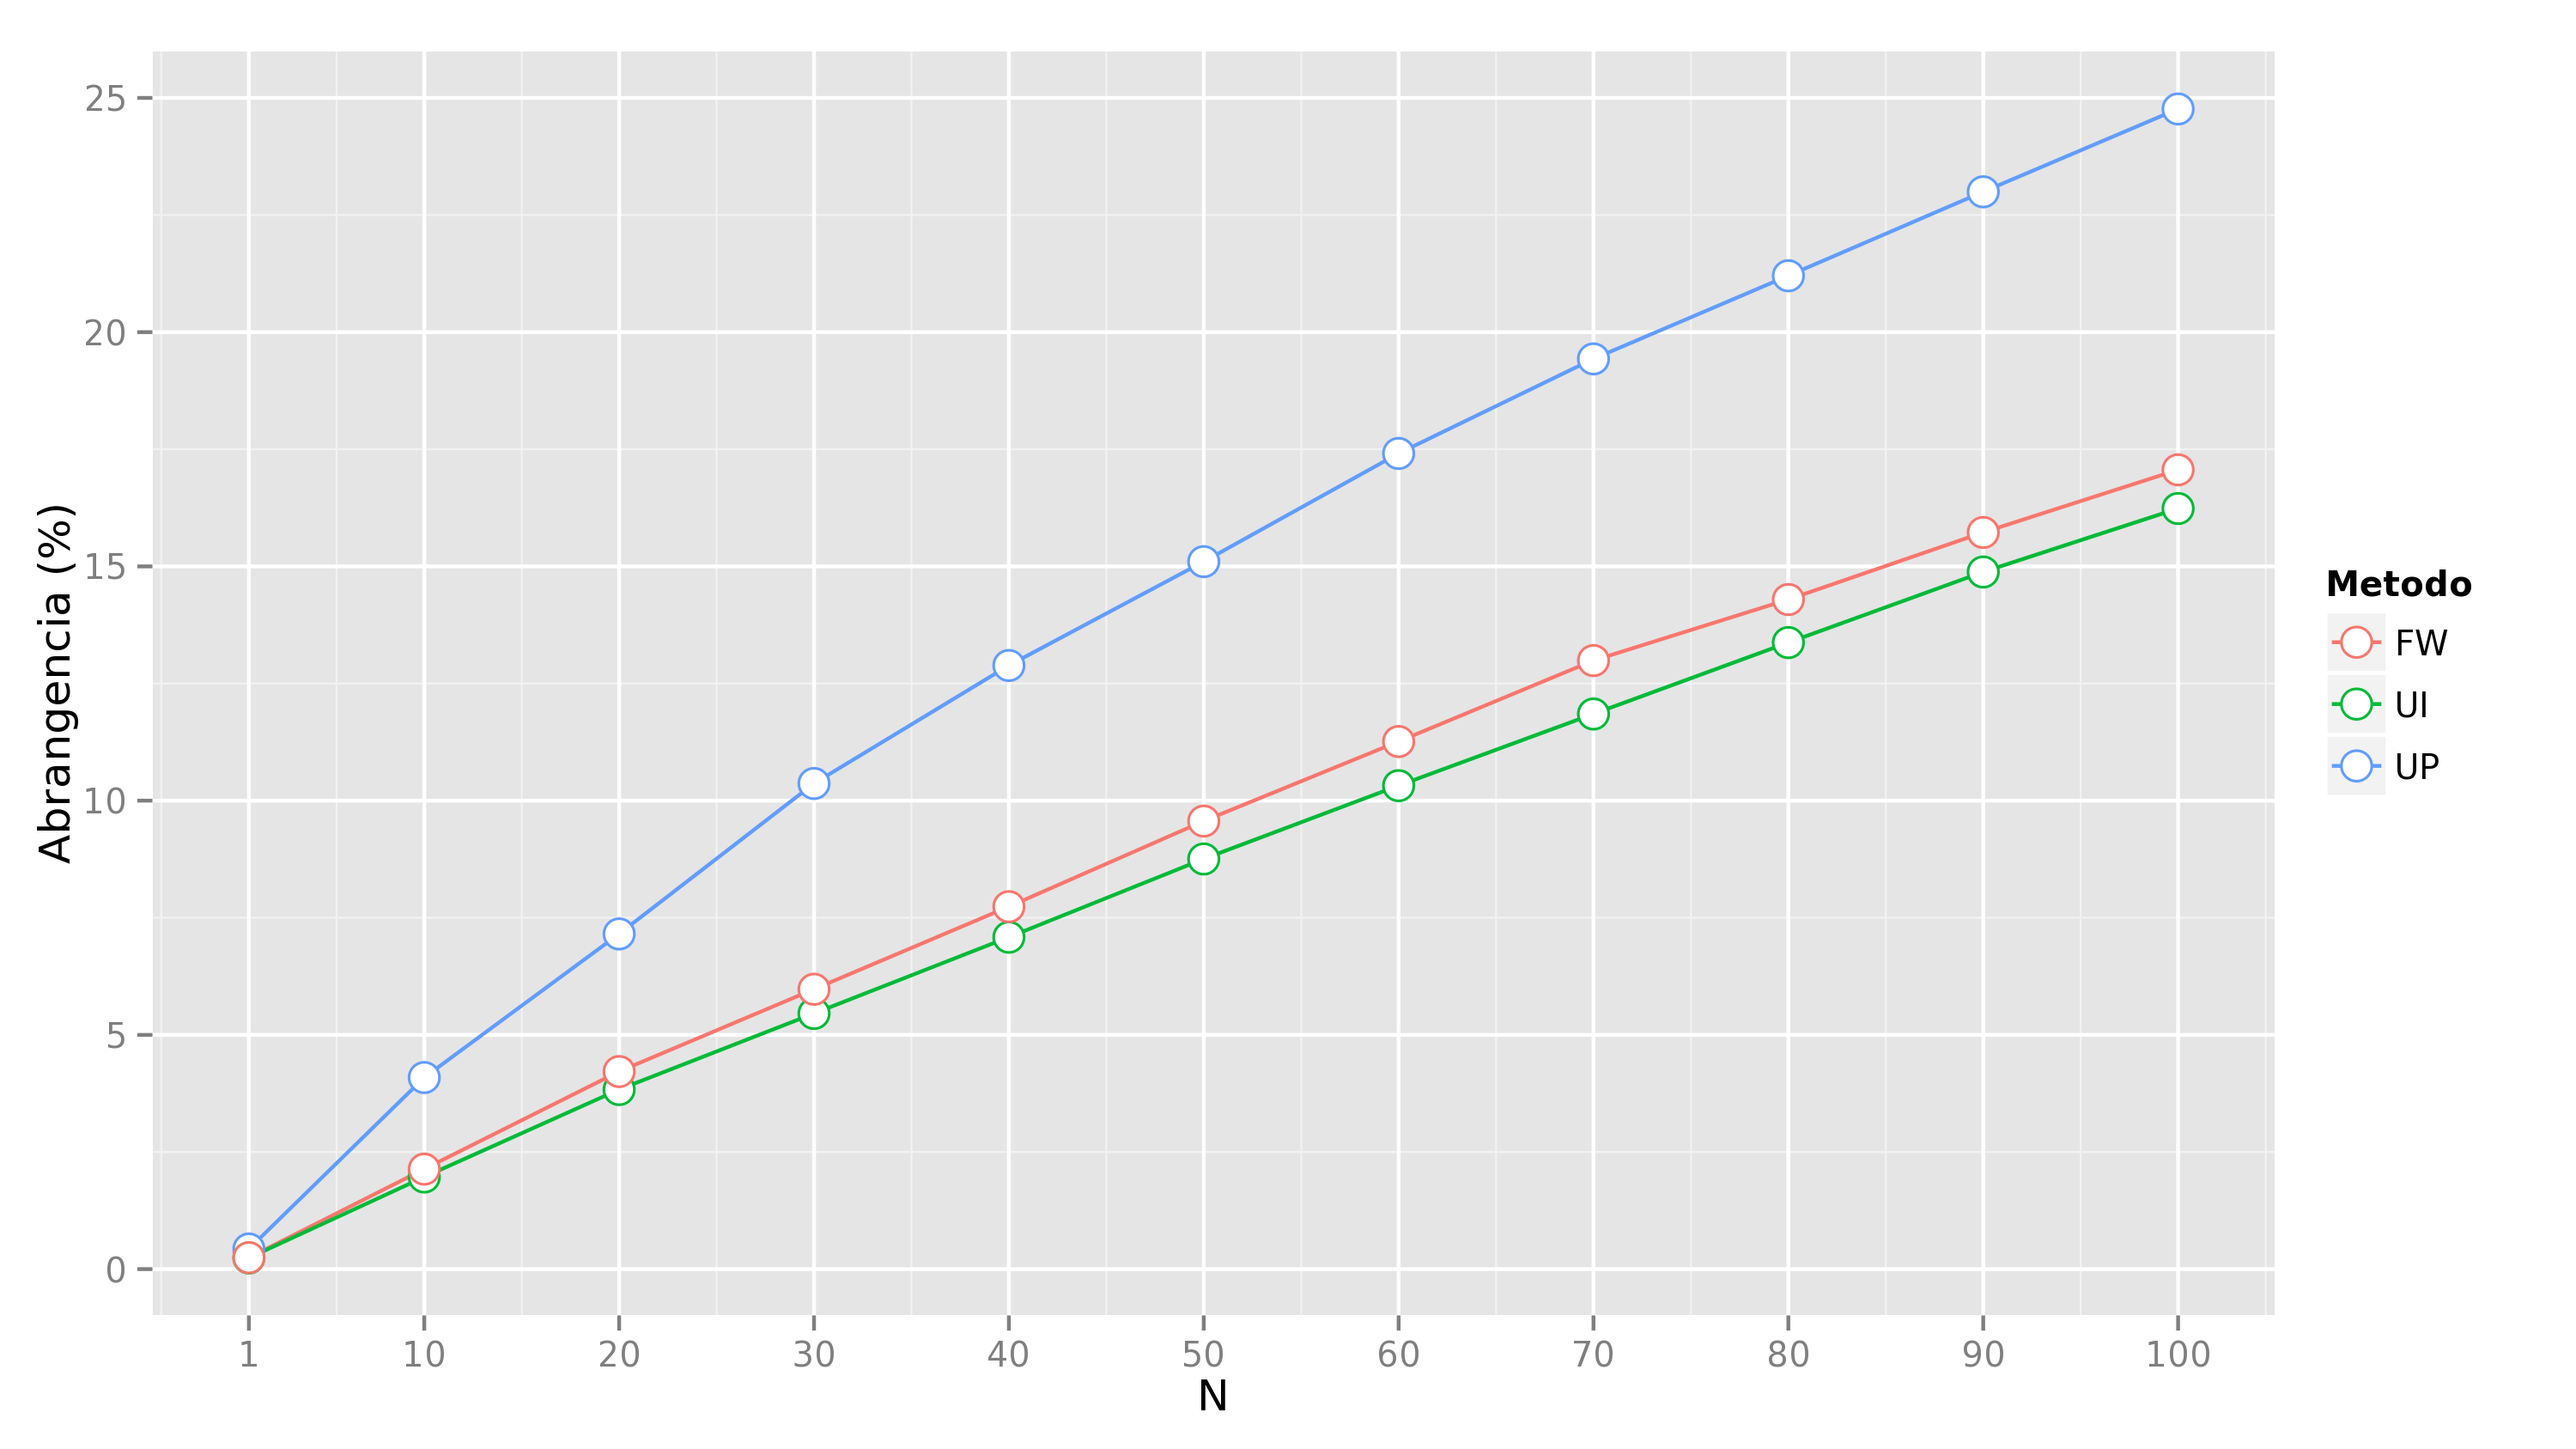
\includegraphics[width=1\textwidth]{img/recall_N_F}
    \end{center}
    \caption{Abrangência em função do tamanho da lista de recomendações $N$}
    \label{fig:recall_N_F}
\end{figure}

\begin{figure}[htp]
    \begin{center}
    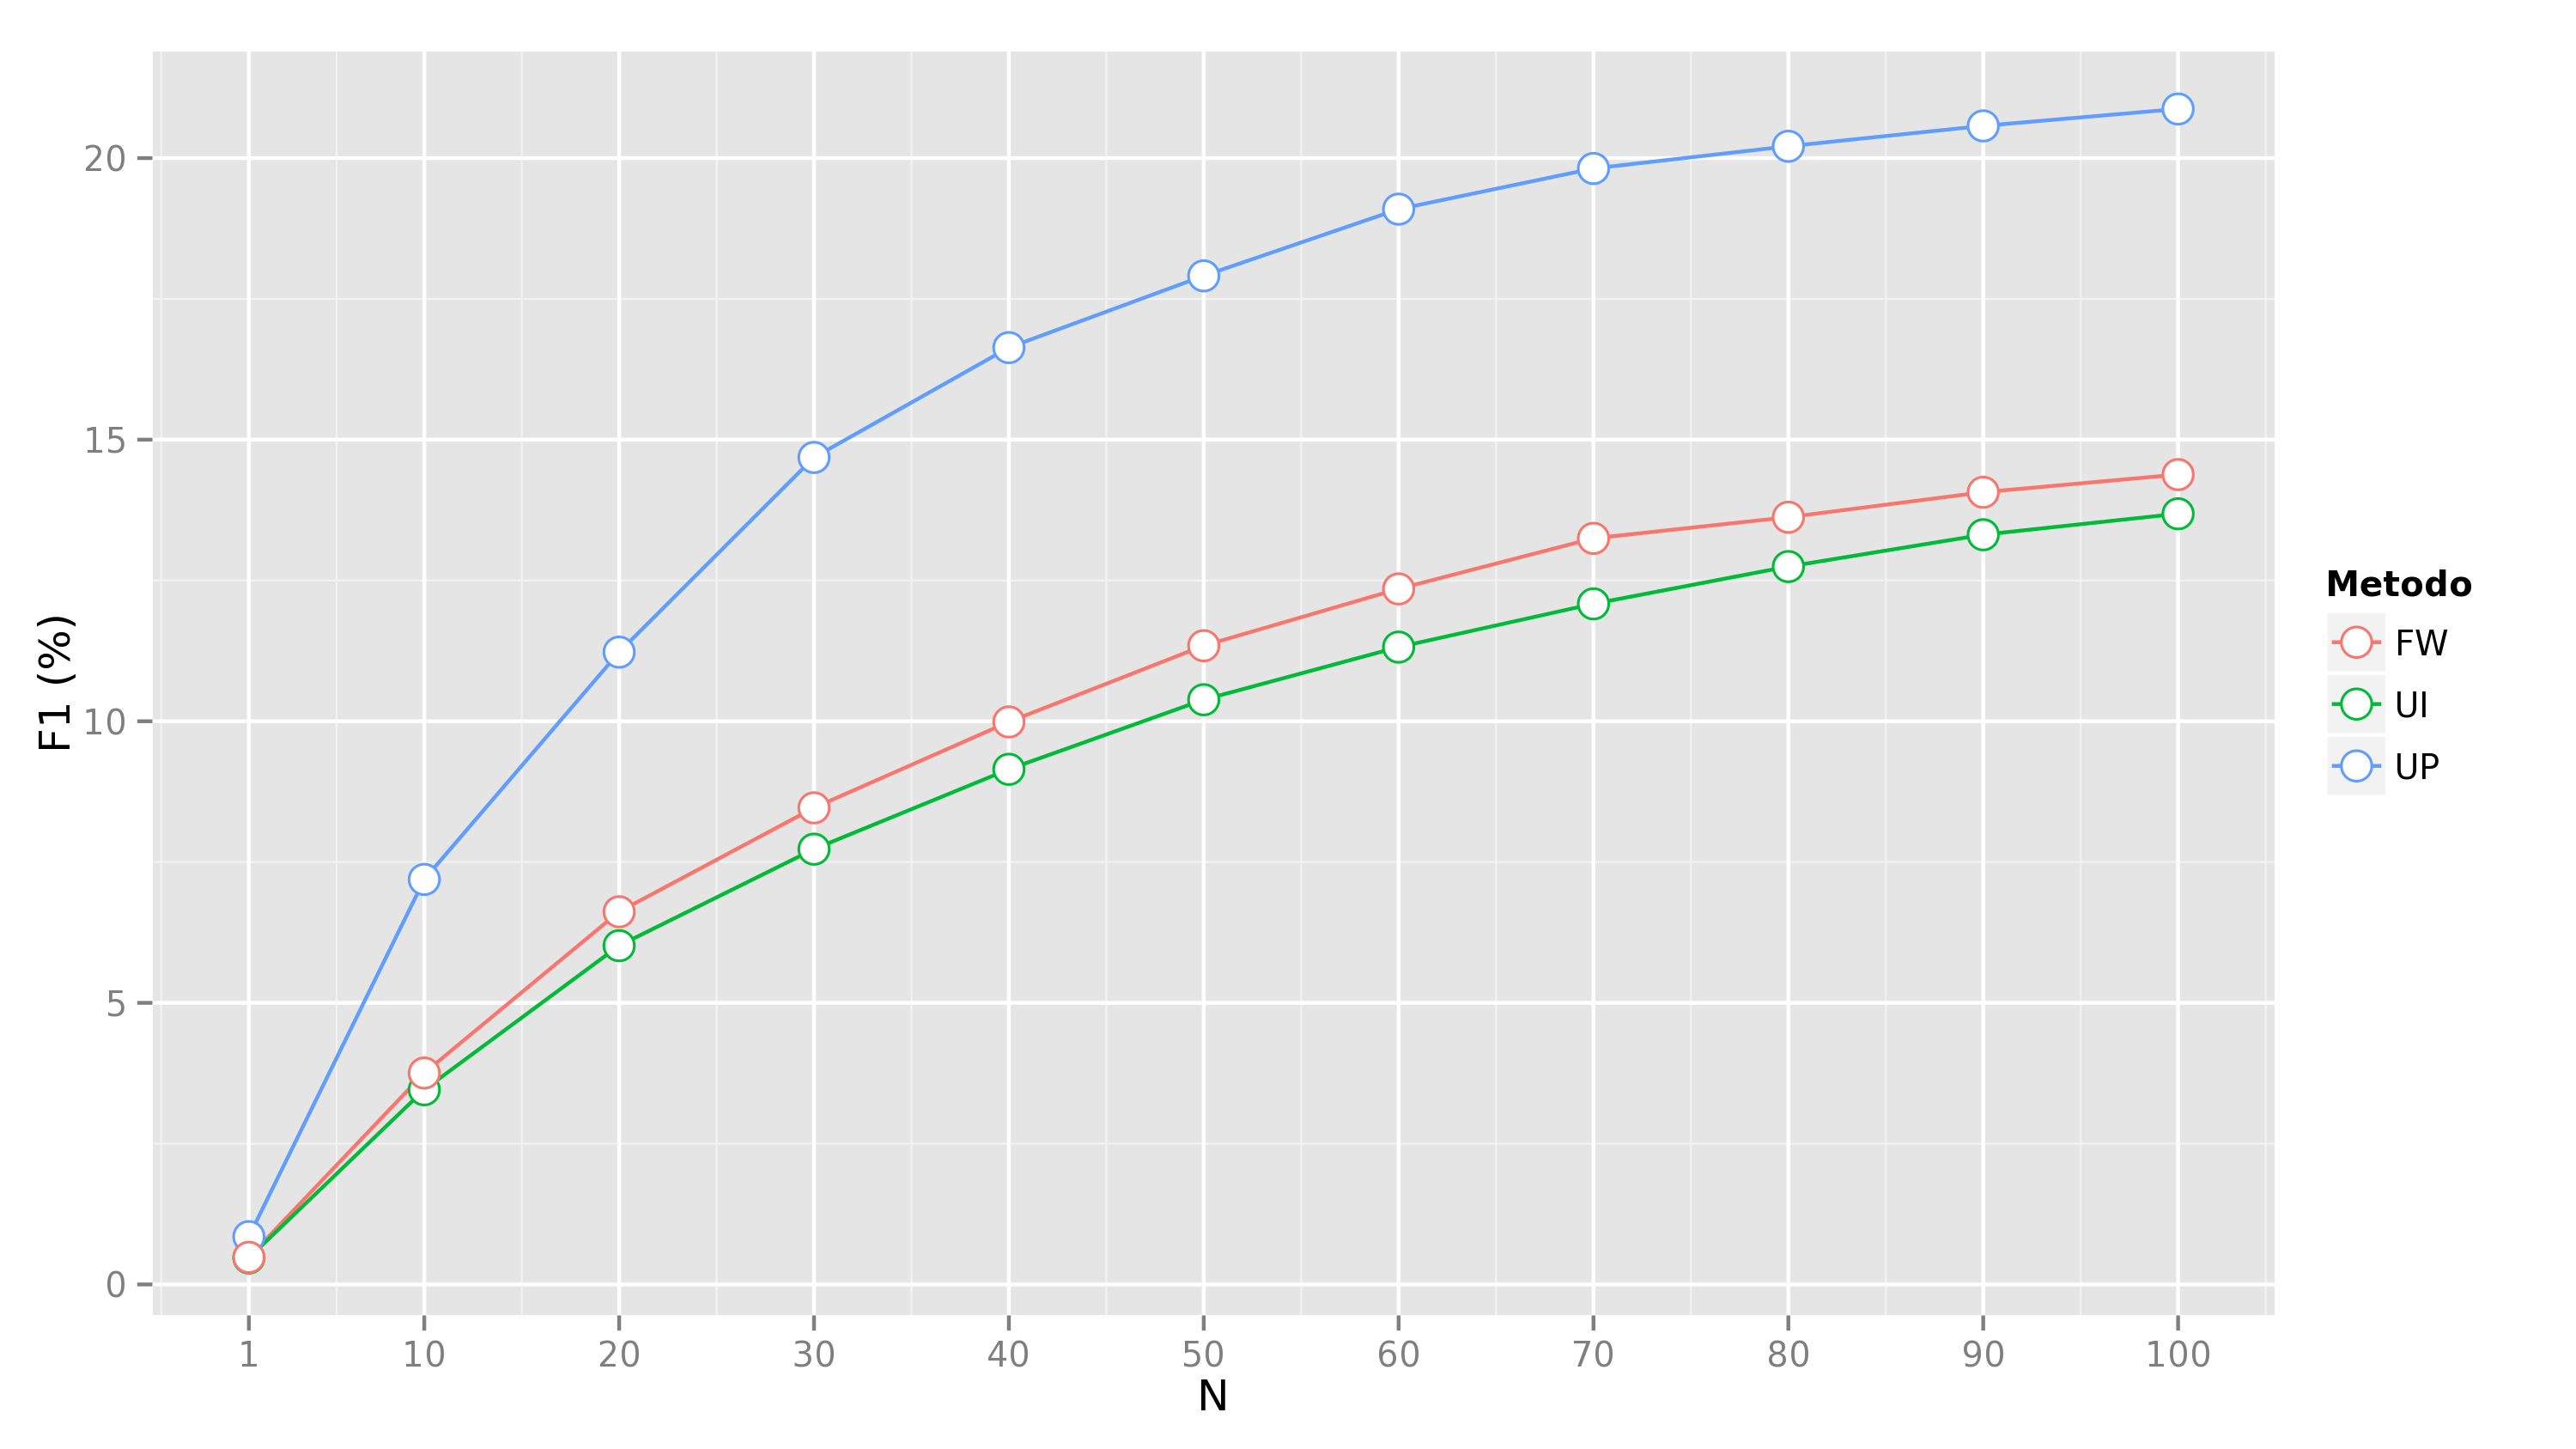
\includegraphics[width=1\textwidth]{img/F1_N_F}
    \end{center}
    \caption{Medida $F_1$ em função do tamanho da lista de recomendações $N$}
    \label{fig:F1_N_F}
\end{figure}

\section{Medida de distância entre atributos $d^f$} % (fold)
\label{sec:medida_de_dist_ncia_entre_atributos_}


\section{Pesos dos atributos $w_f$} % (fold)
\label{sec:pesos_dos_atributos_}

% section pesos_dos_atributos_ (end)

